\documentclass[12pt,a4paper,oneside]{report}        % Single-side
%\documentclass[12pt,a4paper,twoside]{report}  		% Duplex

\usepackage[T1]{fontenc}
\usepackage[utf8]{inputenc}
\usepackage{amsmath}
\usepackage{amssymb}
\usepackage{enumerate}
\usepackage{graphicx}
\usepackage{lastpage}
\usepackage{anysize}
\newcommand\magyarOptions{chapterhead=unchanged}
\usepackage[magyar]{babel}
\usepackage{sectsty}
\usepackage{setspace}
\usepackage{hyperref}
\usepackage{fancyhdr}
\usepackage{titlesec}
\usepackage{pdfpages}
\usepackage[intoc]{nomencl}
\usepackage{lipsum}
\usepackage{float}
\usepackage{caption}
\usepackage{algorithm}
\usepackage{algpseudocode}
\usepackage[a-2b,mathxmp]{pdfx}
\usepackage{longtable}
\usepackage{url}
\usepackage{colortbl}
\usepackage{array}
\usepackage{tikz}
\usepackage{listings}
\usepackage{subcaption}
\usepackage[section]{placeins}
\usepackage{tikz}
\usepackage{adjustbox}
\usetikzlibrary{positioning, calc}
\lstdefinelanguage{GDScript}{
  morekeywords={
    onready, tool, signal, extends, func, var, const, return,
    break, continue, if, elif, else, for, while, match, case, in, 
    and, or, not, pass, preload, is, as, self, true, false, null,
    export, setget, static, enum, class,
	func, if, is, true, false, emit_signal, MOUSE_BUTTON_LEFT, 
    InputEventMouseButton, new_label_text, String
  },
  sensitive=true,
  morecomment=[l]{\#},
  morestring=[b]",
}

\definecolor{codegreen}{rgb}{0,0.6,0}
\definecolor{codegray}{rgb}{0.5,0.5,0.5}
\definecolor{codepurple}{rgb}{0.58,0,0.82}
\definecolor{backcolour}{rgb}{0.95,0.95,0.92}

\lstdefinestyle{mystyle}{
	backgroundcolor=\color{backcolour},   
    commentstyle=\color{codegreen},
    keywordstyle=\color{magenta},
    numberstyle=\tiny\color{codegray},
    stringstyle=\color{codepurple},
    breakatwhitespace=false,         
    breaklines=true,                 
    captionpos=b,                    
    keepspaces=true,                 
    numbers=left,                    
    numbersep=5pt,                  
    showspaces=false,                
    showstringspaces=false,
    showtabs=false,                  
    tabsize=2
}
\lstset{
	style=mystyle,
    basicstyle=\ttfamily\footnotesize,
    basicstyle=\ttfamily,
    breaklines=true,
    numbers=left,
    numberstyle=\tiny,
    frame=single
}



\setlength{\parindent}{12pt}
\setlength{\parskip}{0pt}

\renewcommand{\baselinestretch}{1.5}
\titlespacing*{\section}
{0pt}{5.5ex plus 1ex minus .2ex}{4.3ex plus .2ex}

\marginsize{35.4mm}{25.4mm}{25.4mm}{25.4mm} % anysize package

\titleformat{\chapter}[display]{\fontsize{14}{15} \bfseries}{\thechapter. \chaptername}{15pt}{}
\sectionfont{\fontsize{12}{15}\bfseries}
\subsectionfont{\fontsize{12}{15}\bfseries}

\hypersetup{
	bookmarks=true,            % show bookmarks bar?
	unicode=false,             % non-Latin characters in Acrobat’s bookmarks
	pdftitle={},        % title
	pdfauthor={},    % author
	pdfsubject={}, % subject of the document
	pdfcreator={},   % creator of the document
	pdfproducer={Producer},    % producer of the document
	pdfkeywords={keywords},    % list of keywords
	pdfnewwindow=true,         % links in new window
	colorlinks=true,           % false: boxed links; true: colored links
	linkcolor=black,           % color of internal links
	citecolor=black,           % color of links to bibliography
	filecolor=black,           % color of file links
	urlcolor=black             % color of external links
}

\pagestyle{fancy}
\fancyhf{}
\fancyfoot[C]{\thepage}
\fancyhead[C]{\leftmark}

\fancypagestyle{plain}{%
	\fancyhf{}%
	\fancyfoot[C]{\thepage}%
	\fancyhead{}
	\renewcommand{\headrulewidth}{0pt}
}

\renewcommand{\chaptermark}[1]{%
	\markboth{#1}{}}
\renewcommand{\headrulewidth}{\iffloatpage{0pt}{0.4pt}}

\DeclareMathOperator*{\argmax}{arg\,max}
\DeclareMathOperator*{\argmin}{arg\,min}
%alairasok beszurasa nyilatkozatokra
\newcommand*{\SignatureAndDate}[1]{%
\par\noindent\makebox[3.5in]{}\hfill\makebox[2.0in]{\dotfill}%
\par\noindent\makebox[3.5in]{}\hfill\makebox[1.8in]{#1}
}%

\renewcommand{\nomname}{Jelölésjegyzék}
\makenomenclature
\makeindex

%%%%%%%%%%%%%%%%%%%%%%%%%%%%%%%%%%%%%%%%%%%%%%%%%%%%%%%%%%%%%%%%%%%%%%%%%%%%%%%%%%%%%%%%%%%%%%%%%%%%%
%%%%%% adatok: FONTOS, HOGY MINDEGYIK ADAT UTÁN LEGYEN SPACE! %%%
%%%ez a makró szakasz, NE itt MÓDOSÍTS hanem 110 sortól! %%%%%%%%%%%%%%%%%%%%%%%%%%%%%%%%%%%%
\def\myuni{Pannon Egyetem }
\def\mykar{Műszaki Informatikai Kar }
\def\mytanszek{\textbf{\textcolor{red}{<<tanszék>>}} } %többi tanszék?
\def\mycim{\textbf{\textcolor{red}{<<A szakdolgozat címe - a témakiírással egyezően>>}} }
\def\myszak{\textbf{\textcolor{red}{<<szak>>}} } %Mérnökinformatikus/Gazdaságinformatikus/Programtervező Informatikus/ Villamosmérnöki/Adattudomány
\def\mynev{\textbf{\textcolor{red}{<<hallgató neve>>}} }
\def\myneptun{\textbf{\textcolor{red}{<<Neptun kód>>}} }
\def\myev{\textbf{\textcolor{red}{<<végzés éve>>}} }
\def\mytemavezeto{\textbf{\textcolor{red}{<<témavezető neve>>}} }
\def\mykonzulens{\textbf{\textcolor{red}{<<külső konzulens neve>>, <<intézménye>> }} }
\def\mybelsokonzulens{\textbf{\textcolor{red}{<<Belső konzulens neve>>, <<intézménye>> }} }
\def\mydate{\textbf{\textcolor{red}{<<év. hónap nap>> }} }
\def\myvaros{\textbf{\textcolor{red}{<<hely>>}} }
\def\myvegzettseg{\textbf{\textcolor{red}{<<végzettség>>}} }
\def\mydolgozat{\textbf{\textcolor{red}{<<Szak-/Diplomadolgozat>>}} }
\def\mydolgozategy{\textbf{\textcolor{red}{<<Szak-/Diplomadolgozatot>>}} }

%%%%%%%%% kitöltendő - komment kitöRlése után ez kerül be a dolgozatba, és nem a piros fenti rész %%%%%%%%%%%%%%
%%%%%% FONTOS, HOGY MINDEGYIK ADAT UTÁN LEGYEN SPACE! %%%%%%%%%%%%%%%%%%%%%%%%%%%%%%%%%%%%%%%
%%%%%% A még nem biztos (pl pontos dátum az aláírásnál) részt érdemes még kikommentelve hagyni, így pirossal marad bent a végéig %%%%%%%%
\def\mycim{3D memóriajáték tervezése mesterséges intelligenciával }
\def\mynev{Csesznák Tamás Levente }
\def\myneptun{P8MQG2 }
\def\myev{2024 }
\def\mytemavezeto{Szabó Patrícia }
%\def\mykonzulens{<<külső konzulens neve>>, <<intézménye>> }
%\def\mybelsokonzulens{<<belső konzulens neve>>, <<intézménye>> }
\def\mydate{2024.12.03 }
\def\myvaros{Veszprém }

%%%%%%%% MI használatára vonatkozó nyilatkozat - KÖTELEZŐ VÁLASZTANI! a kommenet vedd ki a helyes nyilatkozat elől.
%%%%%%%%%%%%%%%%%%%%%%%%%%%%%%5

\def\myMIstatement{használtam}
%\def\myMIstatement{nem használtam}


%%%%%%%%% tanszék - megfelelő elől kivenni a kommentet %%%%%%%%%%%%%%%%%%%%%%%
%\def\mytanszek{Alkalmazott Informatikai }
\def\mytanszek{Informatikai Rendszerek és Alkalmazásai }
%\def\mytanszek{Matematika }
%\def\mytanszek{Rendszer- és Számítástudományi }
%\def\mytanszek{Villamosmérnöki és Információs Rendszerek }


%%%%%%%%% szakok - megfelelő elől kivenni a kommentet %%%%%%%%%%%%%%%%%%%%%%%%%%%%%%%%%%%%
    %% Gazdaságinformatikus BSc
%\def\myszak{Gazdaságinformatikus BSc} \def\myvegzettseg{gazdaságinformatikus } \def\mydolgozat{SZAKDOLGOZAT} \mydolgozat1{szakdolgozatot}
    
    %% Mérnökinformatikus BSc
%\def\myszak{Mérnökinformatikus BSc} \def\myvegzettseg{mérnökinformatikus } \def\mydolgozat{SZAKDOLGOZAT} 
\def\myszak{Mérnökinformatikus BSc} \def\myvegzettseg{mérnökinformatikus } \def\mydolgozat{SZAKDOLGOZAT} \def\mydolgozategy{szakdolgozatot }
    %% Programtervező informatikus BSc
%\def\myszak{Programtervező informatikus BSc} \def\myvegzettseg{programtervező informatikus } \def\mydolgozat{SZAKDOLGOZAT} \mydolgozat1{szakdolgozatot}

    %% Villamosmérnöki BSc
%\def\myszak{Villamosmérnöki BSc} \def\myvegzettseg{villamosmérnöki } \def\mydolgozat{SZAKDOLGOZAT} \mydolgozat1{szakdolgozatot}

    %% Mérnökinformatikus MSc
%\def\myszak{Mérnökinformatikus MSc} \def\myvegzettseg{okleveles mérnökinformatikus } \def\mydolgozat{DIPLOMADOLGOZAT} \mydolgozat1{diplomadolgozatot}

    %% Programtervező informatikus MSc
%\def\myszak{Programtervező informatikus MSc} \def\myvegzettseg{okleveles programtervező informatikus } \def\mydolgozat{DIPLOMADOLGOZAT} \mydolgozat1{diplomadolgozatot}

 %% Adattudomány MSc
%\def\myszak{Adattudomány MSc} \def\myvegzettseg{okleveles adattudós } \def\mydolgozat{DIPLOMADOLGOZAT} \mydolgozat1{diplomadolgozatot}




%itt kerülnek becsatolásra a dolgozat egymást követő fejezetei
\begin{document}
	\pagenumbering{arabic}
	\onehalfspacing
	%a fedlappal kezdj
	%\begin{titlepage}
%    \begin{center}
%        \vspace*{\fill}
%        \Huge \textbf{SZAKDOLGOZAT}\\
%        \vspace{10cm}
%        \Large \textbf{Gyurácz Olivér}\\
%        \vspace{1.5cm}
%        \large 2021
%        \vspace*{\fill}
%    \end{center}
%\end{titlepage}
\begin{titlepage}
    \begin{center}
        \vspace*{\fill}
        \large \textbf{\myuni}\\
        \large \mykar\\
        \large \mytanszek Tanszék\\
        \large \myszak \\
        \vspace{2cm}
        \Huge \textbf{\mydolgozat}\\
        \vspace{2cm}
        %a szakdolgozat címe
        \Large \textbf{\mycim}\\
        \vspace{2cm}
        %a dolgozatot készítő hallgató neve
        \Large \textbf{\mynev}\\
        \vspace{2cm}
        %témavezetőjének a neve
        \large Témavezető: \mytemavezeto\\
        \vspace{1cm}
        %ha van, akkor kitöltendő, ha nincs, akkor törölje a következő sort
        %\large Külső/belső konzulens: \mykonzulens\\
        \vspace{1cm}
        % a dolgozat készítésének évszáma
        \large \myev
        \vspace*{\fill}
    \end{center}
\end{titlepage} 
	%a szkennelt témakiírás a következő, amit pdf-ben csatolunk
	%
\includepdf{Temakiiras.pdf}
	%saját nyilatkozatod nyomtatva, aláírva, pdf-be szkennelve csatolandó. A szerkeszthető részt tartalmazó  h_nyilatkozat.tex fájlt nem kell becsatolni, miután az aláírt nyilatkozat csatolásra kerül
	\begin{center}
\textbf{\large{Hallgatói nyilatkozat}}\\[32pt]
\end{center}

\thispagestyle{fancy}
\pagestyle{fancy}
Alulírott \mynev (Neptun kód: \myneptun ) hallgató kijelentem, és a dolgozat feltöltésével egyidejűleg nyilatkozom, hogy a \mycim című \mydolgozategy  (a továbbiakban: dolgozat) a \myuni \mytanszek Tanszékén készítettem a \myvegzettseg oklevél megszerzése érdekében.\par

Kijelentem, hogy a dolgozatban csak a megadott és hivatkozott forrásokat használtam fel, és ezekre a vonatkozó idézési szabályok szerint hivatkoztam.
\vspace{0.6cm}\par

Nyilatkozom, hogy a dolgozat érdemi része saját szellemi alkotásom eredménye, és azt más intézményben, szakon, vagy felsőfokú képesítés megszerzésére nem nyújtottam be. Tudomásul veszem, hogy a plágium vagy szerzői jogsértés esetén a dolgozatom elutasításra kerülhet, és ellenem fegyelmi eljárás indulhat. Tudomásul veszem továbbá, hogy szerzői jogsértés esetén az Egyetem jogosult a dolgozat elérhetőségét korlátozni, valamint eltávolítani a dokumentumot a dolgozatok tárolására szolgáló, a témát vezető szervezeti egység által meghatározott elektronikus zárt rendszerből.
\vspace{0.6cm}\par

Tudomásul veszem továbbá, hogy a Pannon Egyetem a dolgozat eredményeit saját céljaira eltérő írásbeli megállapodás hiányában a Pannon Egyetem Szellemi Tulajdon Kezelési Szabályzatában foglaltaknak megfelelően szabadon felhasználhatja. 
Nyilatkozom, hogy a dolgozat elkészítése során mesterséges intelligencia eszközöket \myMIstatement. 
\vspace{0.6cm}\par


Nyilatkozom, hogy a dolgozat elkészítése során az alábbi táblázatban feltüntetett mesterséges intelligencia eszközöket kizárólag a kutatási, illetve fejlesztési feladat támogatására használtam fel, az érdemi munka, elemzés és következtetések teljes mértékben saját szellemi alkotásomat képezik.\\

%%%ha nem használtál AI-t, a következő sort vedd ki:
A dolgozatban felhasznált mesterséges intelligencia használatot részletező táblázat:\par
\begin{table}[htb!]
\centering
\arrayrulecolor{black}
\begin{tabular}{!{\color{black}\vrule}>{\hspace{0pt}}m{0.24\linewidth}!{\color{black}\vrule}>{\hspace{0pt}}m{0.31\linewidth}!{\color{black}\vrule}>{\hspace{0pt}}m{0.187\linewidth}!{\color{black}\vrule}>{\hspace{0pt}}m{0.160\linewidth}!{\color{black}\vrule}} 
\hline
\textbf{Alkalmazott technológia} & \textbf{Alkalmazás módja} & \textbf{Előállított tartalom} & \textbf{MI használat aránya} \\ 
\hline
ChatGPT o1-preview (OpenAI)  & Angol fordítás & Abstract & 90\% \\ 
\hline
ChatGPT 4o (OpenAI) & Szöveg generálása: tartalmi összefoglaló & 3. fejezet & 70\% \\ 
\hline
ChatGPT 4o (OpenAI) & Kód generálása & Node.js fájl szerver alapjai & 40\% \\ 
\hline
ChatGPT 4o (OpenAI) & Python kód generálása & Flask webszerver alapjai & 70\% \\ 
\hline
ChatGPT 4o (OpenAI) & Python kód generálása & TensorFlow használata & 30\% \\ 
\hline
ChatGPT 4o (OpenAI) & Nyelvi Stilizálás & Teljes dolgozat & 20\% \\ 
\hline
\end{tabular}
\arrayrulecolor{black}
\end{table}




\vspace{2cm}
Dátum: \myvaros, \mydate\\
\vspace{2cm}

\SignatureAndDate{\mynev}

	%\includepdf{Hallgatoi_nyilatkozat.pdf}
	%témavezetőd nyilatkozata nyomtatva, aláírva, pdf-be szkennelve csatolandó. A szerkeszthető oldalt ki kell kapcsolni majd, ha a szkennelt témavezetői nyilatkozatot beszúrta. A beszúráshoz vegye le a % jelet a 94-es és 98-as sorok elől.
	%\begin{center}
\textbf{\large{Témavezetői nyilatkozat}}\\[32pt]
\end{center}

\thispagestyle{fancy}
\pagestyle{fancy}
Alulírott \mytemavezeto témavezető kijelentem, hogy a dolgozatot \mynev a \myuni \mytanszek Tanszékén készítette a \myvegzettseg végzettség megszerzése érdekében.\\

Kijelentem, hogy a dolgozat védésre bocsátását engedélyezem.\\



\vspace{2cm}
Dátum: \myvaros, \mydate\\
\vspace{2cm}

\SignatureAndDate{\mytemavezeto}

	
\includepdf{Temavezetoi_nyilatkozat.pdf}
	%köszönetnyilvánítás csatolása
	\textbf{\large{Köszönetnyilvánítás}}\\[32pt]

\thispagestyle{fancy}
\pagestyle{fancy}

Dolgozatom elkészültével szeretnék köszönetet mondani .....2-3 mondatban megfogalmazva.\\

Ezen kívül szeretnék köszönetet mondani e .. további köszönet akinek szeretné a Hallgató kifejezni.\\

Végül szeretném megköszönni a családomnak és a barátaimnak, amiért mindvégig önzetlenül támogattak célom elérésében.\\
\\

	%tartalmi összefoglalók csatolása, ami magyar és angol nyelven az Abstract.tex fájlban lesz megírva
	\textbf{\large{Tartalmi összefoglaló}}\\[32pt]

\thispagestyle{fancy}
\pagestyle{fancy}



\vspace{8pt}

Tartalmi összefoglaló magyarul. Az összefoglalónak tartalmaznia kell (rövid, velős és összefüggő megfogalmazásban) a következőket:
\begin{itemize}
    \item téma megnevezése,
    \item megoldott feladat megfogalmazása,
    \item megoldási mód,
    \item elért eredmények,
    \item kulcsszavak (4-6 darab).
\end{itemize}
A tartalmi összefoglaló terjedelme nem lehet több egy A4-es oldalnál.\par
Az összefoglalót magyar és angol nyelven kell készíteni. Sorrendben a dolgozat nyelvével megegyező kerül előrébb. A cím Title stílusú, formázása: Times New Roman/ Computer Modern, nagybetű, 14 pt, félkövér, középre igazított; az összefoglaló szövege Normál stílusú, formázása: Times New Roman, 12 pt, sorkizárt, 1.5-ös sortávolság.

\vspace{8pt}



\textbf{Kulcsszavak: } Kulcsszó1, kulcsszó2, kulcsszó3, kulcsszó4, kulcsszó5, kulcszó6

\newpage



\textbf{\large{Abstract}}\\[32pt]

\thispagestyle{fancy}
\pagestyle{fancy}

\vspace{8pt}

Tartalmi összefoglaló angol nyelven, a tartalma és formázása megegyezik a magyar nyelvű tartalmi összefoglalóval.

\vspace{8pt}


\textbf{Keywords: } Keyword1, Keyword2, Keyword3, Keyword4, Keyword5, Keyword6 
	%Tartalomjegyzéket a Tex generálja, nem kell szerkeszteni
	\tableofcontents\vfill
	\addtocontents{toc}{\protect\thispagestyle{empty}}
	\pagestyle{empty}
	%rövidítések jegyzése a Jelolesjegyzek.tex fájlban szerkesztendő
	
%\nomenclature{$U$}{Feszültség}
%\nomenclature{$\boldsymbol{x}$}{Állapotvektor}
%\nomenclature{$\boldsymbol{A}$}{Incidencia mátrix}


\nomenclature{$AI$}{Artificial Intelligence - Mesterséges Intelligencia}
\nomenclature{$MI$}{Mesterséges Intelligencia}
% \nomenclature{$GPU$}{Graphical Processing Unit (Grafikus Processzor / Grafikus Feldolgozó Egység)}
\nomenclature{$API$}{Application Programming Interface (Alkalmazásprogramozási Felület)}
\nomenclature{$2D$}{Kettő dimenziós}
\nomenclature{$3D$}{Három dimenziós}
\nomenclature{$IDE$}{Integrált fejlesztői környezet}
\nomenclature{$ReLU$}{Rectified Linear Unit - Rektifikált lineáris egység}
\nomenclature{$mse$}{mean squared error - átlagos négyzetes hiba}
\nomenclature{$HTML$}{Hypertext Markup Language}
\nomenclature{$SUS$}{System Usability Scale}
\nomenclature{$HTML5$}{Hypertext Markup Language 5}
\nomenclature{$npm$}{Node Package Manager}
\nomenclature{$JSON$}{JavaScript Object Notation}
\nomenclature{$ID$}{Identification - azonosító}
\nomenclature{$NoSQL$}{Not Only SQL (Structured Query Language)}
\nomenclature{$IndexedDB$}{Indexed Data Base}
\nomenclature{$UEQ$}{User Experience Questionnaire}
\nomenclature{$SUS$}{System Usability Scale}
% \nomenclature{$CPU$}{Central Processing Unit (Központi Feldolgozó Egység / Processzor)}
% \nomenclature{$GUI$}{Graphical User Interface (Grafikus Felhasználói Felület)}
% \nomenclature{$HCI$}{Human Computer Interaction (Ember-gép kapcsolat)}
% \nomenclature{$CIS$}{Cognitive Information System (Kognitív információs rendszer)}



\cleardoublepage
\markboth{\nomname}{\nomname}% maybe with \MakeUppercase
\printnomenclature
\thispagestyle{plain}
\nomenclature{}{\pagestyle{plain}}



%fordítás: terminálban:

%pdflatex document.tex
%makeindex document.nlo -s nomencl.ist -o document.nls
%pdflatex document.tex

	%dolgozat fejezetei, amit a HALLGATÓ MEGÍR. A fejezetek tetszőleges néven létrehozhatók, fejezetnev.tex formátumban, a dokumentumba befordításuk az itt megadott sorrendben történik.
	\chapter{Bevezetés}
\usetikzlibrary{shapes,arrows}

\thispagestyle{fancy}
\pagestyle{fancy}
\section{Projekt célja}
A jelenlegi kor társadalmi és technológiai kihívásai közepette egyre fontosabbá válik az emberiség számára az olyan innovatív megoldások keresése, amelyek segíthetnek fejleszteni és támogatni az emberek mindennapi életét. Az Artificial Intelligence (AI), vagyis a Mesterséges Intelligencia, ebben az összefüggésben különösen figyelemre méltó tényezővé vált. Bár sokan aggódnak amiatt, hogy az AI alkalmazása az emberi társadalom hanyatlásához vezethet, én úgy vélem, hogy a megfelelő módon felhasználva az AI lehetőségei elősegíthetik a társadalmi fejlődést és előnyöket hozhatnak az emberi élet számos területén.

Szakdolgozatom központi célja az, hogy az AI alkalmazásával támogassam embertársaim rövidtávú memóriájának fejlesztését. Ehhez egy saját fejlesztésű virtuális valóság alapú, három dimenziós memóriajátékot tervezek létrehozni, amely segítségével interaktív és hatékony módon lehet fejleszteni a játékosok kognitív képességeit. 
\section{Projet bemutatása}
\begin{figure}
    \centering
        \begin{tikzpicture}[>=latex',node distance=2cm,auto]
        % Define block styles
        \tikzstyle{block} = [rectangle, draw, text width=3cm, text centered, minimum height=1.5cm ]
        \tikzstyle{line} = [draw, -latex']

        % Nodes
        \node [block] (kutatomunka) {Kutatómunka};
        \node [block, below of=kutatomunka, node distance=3cm] (tervezes) {Játék megtervezése};
        \node [block, below of=tervezes, node distance=3cm] (jatek_megirasa) {Játék fejlesztése};
        \node [block, below of=jatek_megirasa, node distance=3cm] (adatgyujtes) {Adatgyűjtés webalkalmazás segítségével};
        \node [block, below of=adatgyujtes, node distance=3cm] (MI) {MI modell betanítása};
        \node [block, below of=MI, node distance=3cm] (MI_ember) {MI játszatása ember ellen};

        % \node [block, right of=section1, node distance=4cm] (subsection1) {Subsection 1};
        % \node [block, right of=section2, node distance=4cm] (subsection2) {Subsection 2};

        % Arrows
        \path [line] (kutatomunka) -- (tervezes);
        \path [line] (tervezes) -- (jatek_megirasa);
        \path [line] (jatek_megirasa) -- (adatgyujtes);
        \path [line] (adatgyujtes) -- (MI); 
        \path [line] (MI) -- (MI_ember);

    \end{tikzpicture}
    \caption{Projekt folyamatábrája}
    \label{fig:folyamat_diagram}
\end{figure}
projektem több feladatból állt, melyet egy folyamatdiagram (\ref{fig:folyamat_diagram} ábra) szemléltet.

\subsection{Kutatómunka}
A kutatómunka során elsősorban azt vizsgáltam, hogy melyik tanító algoritmussal érhetem el a kívánt eredményt. Különböző irodalmakat tanulmányoztam, valamint áttekintettem mások munkáit a témában. A kutatómunka végeztével összegeztem a talált eredményeket.

\subsection{Játék megtervezése}
A kutatómunka után el kellett döntenem, hogy milyen játékot fejlesztek, amely elég bonyolult ahhoz, hogy kihívást jelentsen a játékosok számára, ugyanakkor elég egyszerű ahhoz, hogy az AI betanítása belátható időn belül megtörténjen. Ezen a ponton meg kellett azt is határoznom, hogy milyen technológiát alkalmazok, valamint hogy mely területekre összpontosítok a fejlesztés folyamán.

\subsection{Játék lefejlesztése}
A megfelelő tervezés után lefejlesztettem a választott fejlesztői környezetben a játékot. A fejlesztés során két fontos szempontot tartottam szem előtt: a játékot lehetővé kell tenni virtuális valóságban és asztali számítógépen egyaránt, valamint biztosítanom kell, hogy az AI képes legyen kezelni a játékot csupán a játék metainformációinak ismeretében.

\subsection{Adatgyűjtés és VR támogatás}
Miután elkészült a játék, több különböző korosztállyal játszattam azt annak érdekében, hogy elegendő adatom legyen az AI betanításához. Ebben az időszakban foglalkoztam a játék VR támogatásának fejlesztésével is.

\subsection{AI betanítása}
A gyűjtött adatokat felhasználva betanítottam az AI-t egy tanító algoritmus segítségével.

\subsection{AI játszatása}
A játékhoz létrehoztam egy interfészt, amely lehetővé tette az AI számára, hogy játszhasson vele. Miután ez sikeresen működött, lehetőséget teremtettem arra is, hogy az emberi játékos a gép ellen is játszhassa a játékot.

	\chapter{Irodalomkutatás}

\thispagestyle{fancy}
\pagestyle{fancy}

\vspace{8pt}
\section{}


	\chapter{Felhasznált technológiák}

\thispagestyle{fancy}
\pagestyle{fancy}

Munkám során törekedtem arra, hogy a felhasznált technológiákat lehetőleg minimalizáljam. 
Figyelembe vettem továbbá azt is, hogy nyílt forráskódú, és multiplatform eszközöket válasszak. Ezen döntések lehetővé tették számomra a kellő flexibilitást, és elősegítették a munkámat.
\section{Godot Engine}
A Godot egy nyílt forráskódú, ingyenesen elérhető játékmotor és fejlesztői környezet, amelyet a játékok, interaktív tartalmak és egyéb multimédiás alkalmazások létrehozására terveztek. A motorot Juan Linietsky, Ariel Manzur és George Marques alapította 2014-ben, és azóta folyamatos fejlesztés alatt áll, számos kiadott verzióval és fejlesztői közösséggel.

A Godot kiemelkedik sokoldalúsága és könnyűsége miatt. Az egyik legfontosabb jellemzője az integrált fejlesztői környezet (IDE), amely segítségével a fejlesztők egyetlen alkalmazásban végezhetik el a játékterv készítését, a kódolást, a grafika létrehozását és a játéktesztek futtatását. Az IDE rendelkezik számos funkcióval, mint például kódszerkesztő, jelenet szerkesztő, animációkészítő, fizikai motor, hangkezelő, és még sok más, amelyek egyszerűsítik és gyorsítják a fejlesztési folyamatot.

A Godot támogatja a kettő dimenziós (2D) és a három dimenziós (3D) játékfejlesztést is, és számos előre elkészített funkciót és sablont kínál mindkét típushoz. A motor különösen erős a vizuális effektek, az animációk és a szkriptelés terén, és lehetővé teszi a fejlesztők számára, hogy rugalmasan alkalmazzák saját ötleteiket és terveiket a játék készítése során.
 
A Godot-t széles körben használják különböző projektekben, beleértve az indie játékokat, oktatási alkalmazásokat, interaktív médiaalkotásokat. A motor aktív és elkötelezett fejlesztői közösséggel rendelkezik, amely folyamatosan hozzájárul az új funkciók, javítások és dokumentációk fejlesztéséhez.

Megvizsgáltam a további lehetősségeimet is. Használhattam volna Unreal Engine-t, mely egy magas szintű 3D játékok fejlesztésére szakosodott játékmotor.
Azonban túl nagy volt a rendszerkövetelménye. A másik lehetősségem a Unity volt.
Összehasonlítottam a Unity-t a Godot-al és arra jutottam, hogy a Godot GDScript nyelve sokkal könnyebben használható, így végül a Godot mellett döntöttem. 

\section{GDScript}
A GDScript a Godot Engine saját szkriptelési nyelve, amelyet a játékfejlesztéshez terveztek. 
Könnyen tanulható és használható nyelv, amelyet kifejezetten a Godot-hoz optimalizáltak, így tökéletesen illeszkedik a motor által nyújtott funkciókhoz és struktúrához.

A GDScript egy dinamikus típusú script nyelv, ezáltal egyszerűbb és rugalmasabb kódolási stílust tesz lehetővé, amely könnyen alkalmazható a játékfejlesztés során.

Támogatja az objektumorientált programozás alapvető elveit, mint például az osztályok, az öröklődés és a polimorfizmus. Emellett rendelkezik számos beépített funkcióval és osztállyal, melyek jelentősen megkönnyítik a játékprogram készítését.

\section{itch.io}
Az itch.io (kisbetűs írásmóddal) egy web platform, ahol a felhasználók, és fejlesztők indie videojátékokat, szerepjátékokat, játékelemeket, képregényeket, és zeneszámokat oszthatnak meg, árusíthatnak és tölthetnek le. A weboldalt Leaf Corcoran indította 2013 márciusában, és 2023 áprilisi állapot szerint több mint 700,000 termék található rajta.

Az itch.io támogatja, hogy HTML5-be kiexportált játékokat és feltöltött játékokat a böngészőből bárki játszhassa, egy gombnyomással.

\section{CloudFlair}
A Cloudflare Tunnel egy biztonságos és megbízható megoldás, amely lehetővé teszi, hogy a helyi szervereket nyilvános domain név alatt érjük el, anélkül, hogy közvetlenül kinyitnánk a tűzfalat. Ez jelentősen növeli a biztonságot, mivel a szerver közvetlenül nem lesz kitéve az internet veszélyeinek, miközben a szolgáltatás könnyen elérhető marad.

\section{NodeJS}
A Node.js egy nyílt forráskódú, platformfüggetlen JavaScript futtatókörnyezet, amely a V8 JavaScript motort használja. A Node.js lehetővé teszi a fejlesztők számára, hogy szerveroldali alkalmazásokat készítsenek JavaScript nyelven. Egyedülálló eseményvezérelt, nem-blokkoló I/O modellt alkalmaz, amely rendkívül hatékony és alkalmas adatintenzív valós idejű alkalmazások fejlesztésére. A Node.js ökoszisztémája rendkívül gazdag, köszönhetően a npm (Node Package Manager) csomagkezelőnek, amely több százezer ingyenesen elérhető modul közül válogathat.

\section{Docker}
A Docker egy nyílt forráskódú platform, amely lehetővé teszi az alkalmazások konténerizálását, skálázhatóságát és hordozhatóságát. A Docker konténerek könnyű, elszigetelt környezeteket biztosítanak, amelyekben az alkalmazások futtathatók. Ezek a konténerek tartalmazzák az összes szükséges függőséget és konfigurációt, így az alkalmazások bármilyen környezetben, változtatás nélkül futtathatók. A Docker egyszerűvé teszi az alkalmazások telepítését és frissítését, miközben minimalizálja az „egy gépen működik, de másikon nem” problémákat. A Docker Compose lehetőséget biztosít több konténer egyidejű kezelésére és orkestrációjára, ami különösen hasznos komplex alkalmazások esetében.

\section{Express}
Az Express.js, vagy egyszerűen Express, egy minimalista és rugalmas Node.js webalkalmazás keretrendszer, amely gazdag funkcionalitással rendelkezik webalkalmazások és API-k fejlesztéséhez. Az Express leegyszerűsíti a szerver felépítését és konfigurálását, és számos köztes réteget (middleware) kínál, amelyek megkönnyítik a különböző feladatok kezelését, mint például az adatfeldolgozás, az autentikáció, a session kezelés, és a fájlkezelés. Az Express előnye, hogy könnyen bővíthető és integrálható más modulokkal és eszközökkel, ami gyors és hatékony fejlesztést tesz lehetővé.

\section{Python 3}
A Python 3 egy magas szintű, dinamikusan típusos programozási nyelv, amely 2008-ban jelent meg. Egyszerű és olvasható szintaxisával, valamint széleskörű könyvtáraival gyorsan népszerűvé vált. Támogatja az objektumorientált programozást és különböző alkalmazási területekhez, például webfejlesztéshez, adatfeldolgozáshoz és gépi tanuláshoz kínál eszközöket. Keresztplatformos működése miatt könnyen használható különböző operációs rendszereken, és aktív közössége folyamatosan bővíti és fejleszti.

\section{Tensorflow}
A TensorFlow \cite{tensorflow2015-whitepaper} egy nyílt forráskódú szoftverkönyvtár gépi tanuláshoz és mesterséges intelligenciához. Eredetileg a Google Brain csapat fejlesztette, és mára az egyik legnépszerűbb és legszélesebb körben használt keretrendszer a gépi tanulási modellek fejlesztéséhez és futtatásához. A TensorFlow rugalmas és moduláris architektúrája lehetővé teszi a különböző típusú neurális hálózatok könnyű fejlesztését és tréningezését. Különféle eszközöket és könyvtárakat kínál, amelyek támogatják a mély tanulási, természetes nyelvfeldolgozási, és kép-felismerési feladatokat. A TensorFlow-t széles körben használják kutatók és ipari szakemberek egyaránt a mesterséges intelligencia és gépi tanulás területén.

\section{Keras}
A Keras egy könnyen használható API, amely a TensorFlow alapjaira épül, és leegyszerűsíti a mélytanulási modellek fejlesztését. Segítségével gyorsan és egyszerűen lehet modelleket létrehozni, tesztelni és tanítani, ami különösen hasznos prototípusok készítésekor és kísérletezéskor. Kihasználja a TensorFlow erejét és rugalmasságát, miközben felhasználóbarát marad.

\section{SHA256}
Az SHA-256 egy hash-függvény, amely bármilyen méretű adatot 256 bites (32 bájtos) kóddá alakít. Széles körben használják biztonsági alkalmazásokban, például digitális aláírásokban és adatintegritás ellenőrzésére. Az SHA-256 az SHA-2 család tagja, és erős kriptográfiai tulajdonságai miatt nehéz visszafejteni vagy ütközéseket találni.

\section{Flask}
A Flask egy könnyű és rugalmas webkeretrendszer Python nyelvhez, amely lehetővé teszi gyors webalkalmazások fejlesztését. 2010-ben indult, és mikrokeretrendszerként minimalista alapokkal rendelkezik, de könnyen bővíthető különböző modulokkal. Fő jellemzői közé tartozik az egyszerűség, rugalmasság és a RESTful API-k támogatása. Ideális választás egyszerű webalkalmazásokhoz, prototípusokhoz és nagyobb projektekhez is a megfelelő bővítmények segítségével.

\section{ChatGPT}
A ChatGPT az OpenAI által fejlesztett mesterséges intelligencia alapú nyelvi modell, amely természetes nyelven folytat beszélgetéseket. Képes megérteni a felhasználói kérdéseket, és releváns válaszokat generálni széleskörű tudásbázisából. Interaktív és kontextusérzékeny, így alkalmazható információkeresésre, kreatív írásra és sok más feladatra. Folyamatosan fejlődik, hogy javítsa a felhasználói élményt.

A projektemben a ChatGPT-t felhasználtam, hogy a szakdolgozatomat stilisztikailag kijavítsa, a formázás szempontjából felgyorsítsa az írás folyamatát. Használtam a mesterséges inteligencia tanító kódjának leírásához, mint iránymutató, valamint a webapplikáció elkészítésében is a segítségét kértem. Ezeken kívűl mint fordító is használtam, hogy az angol dokumentációkat magyarra fordítsam. 
	\chapter{A játék működése}

\thispagestyle{fancy}
\pagestyle{fancy}
\section{Játék ismertetése}

A játék melyet lefeljleszettem, a közismert memória játék. A játékot lehet egyedül, vagy akár többen is játszani.

A játékban, egy asztalon meghatározott számú kártya pár található, képpel lefelé fordítva ahogyan az a \ref{img:asztal}. ábrán is látható.
\begin{figure}[h]
    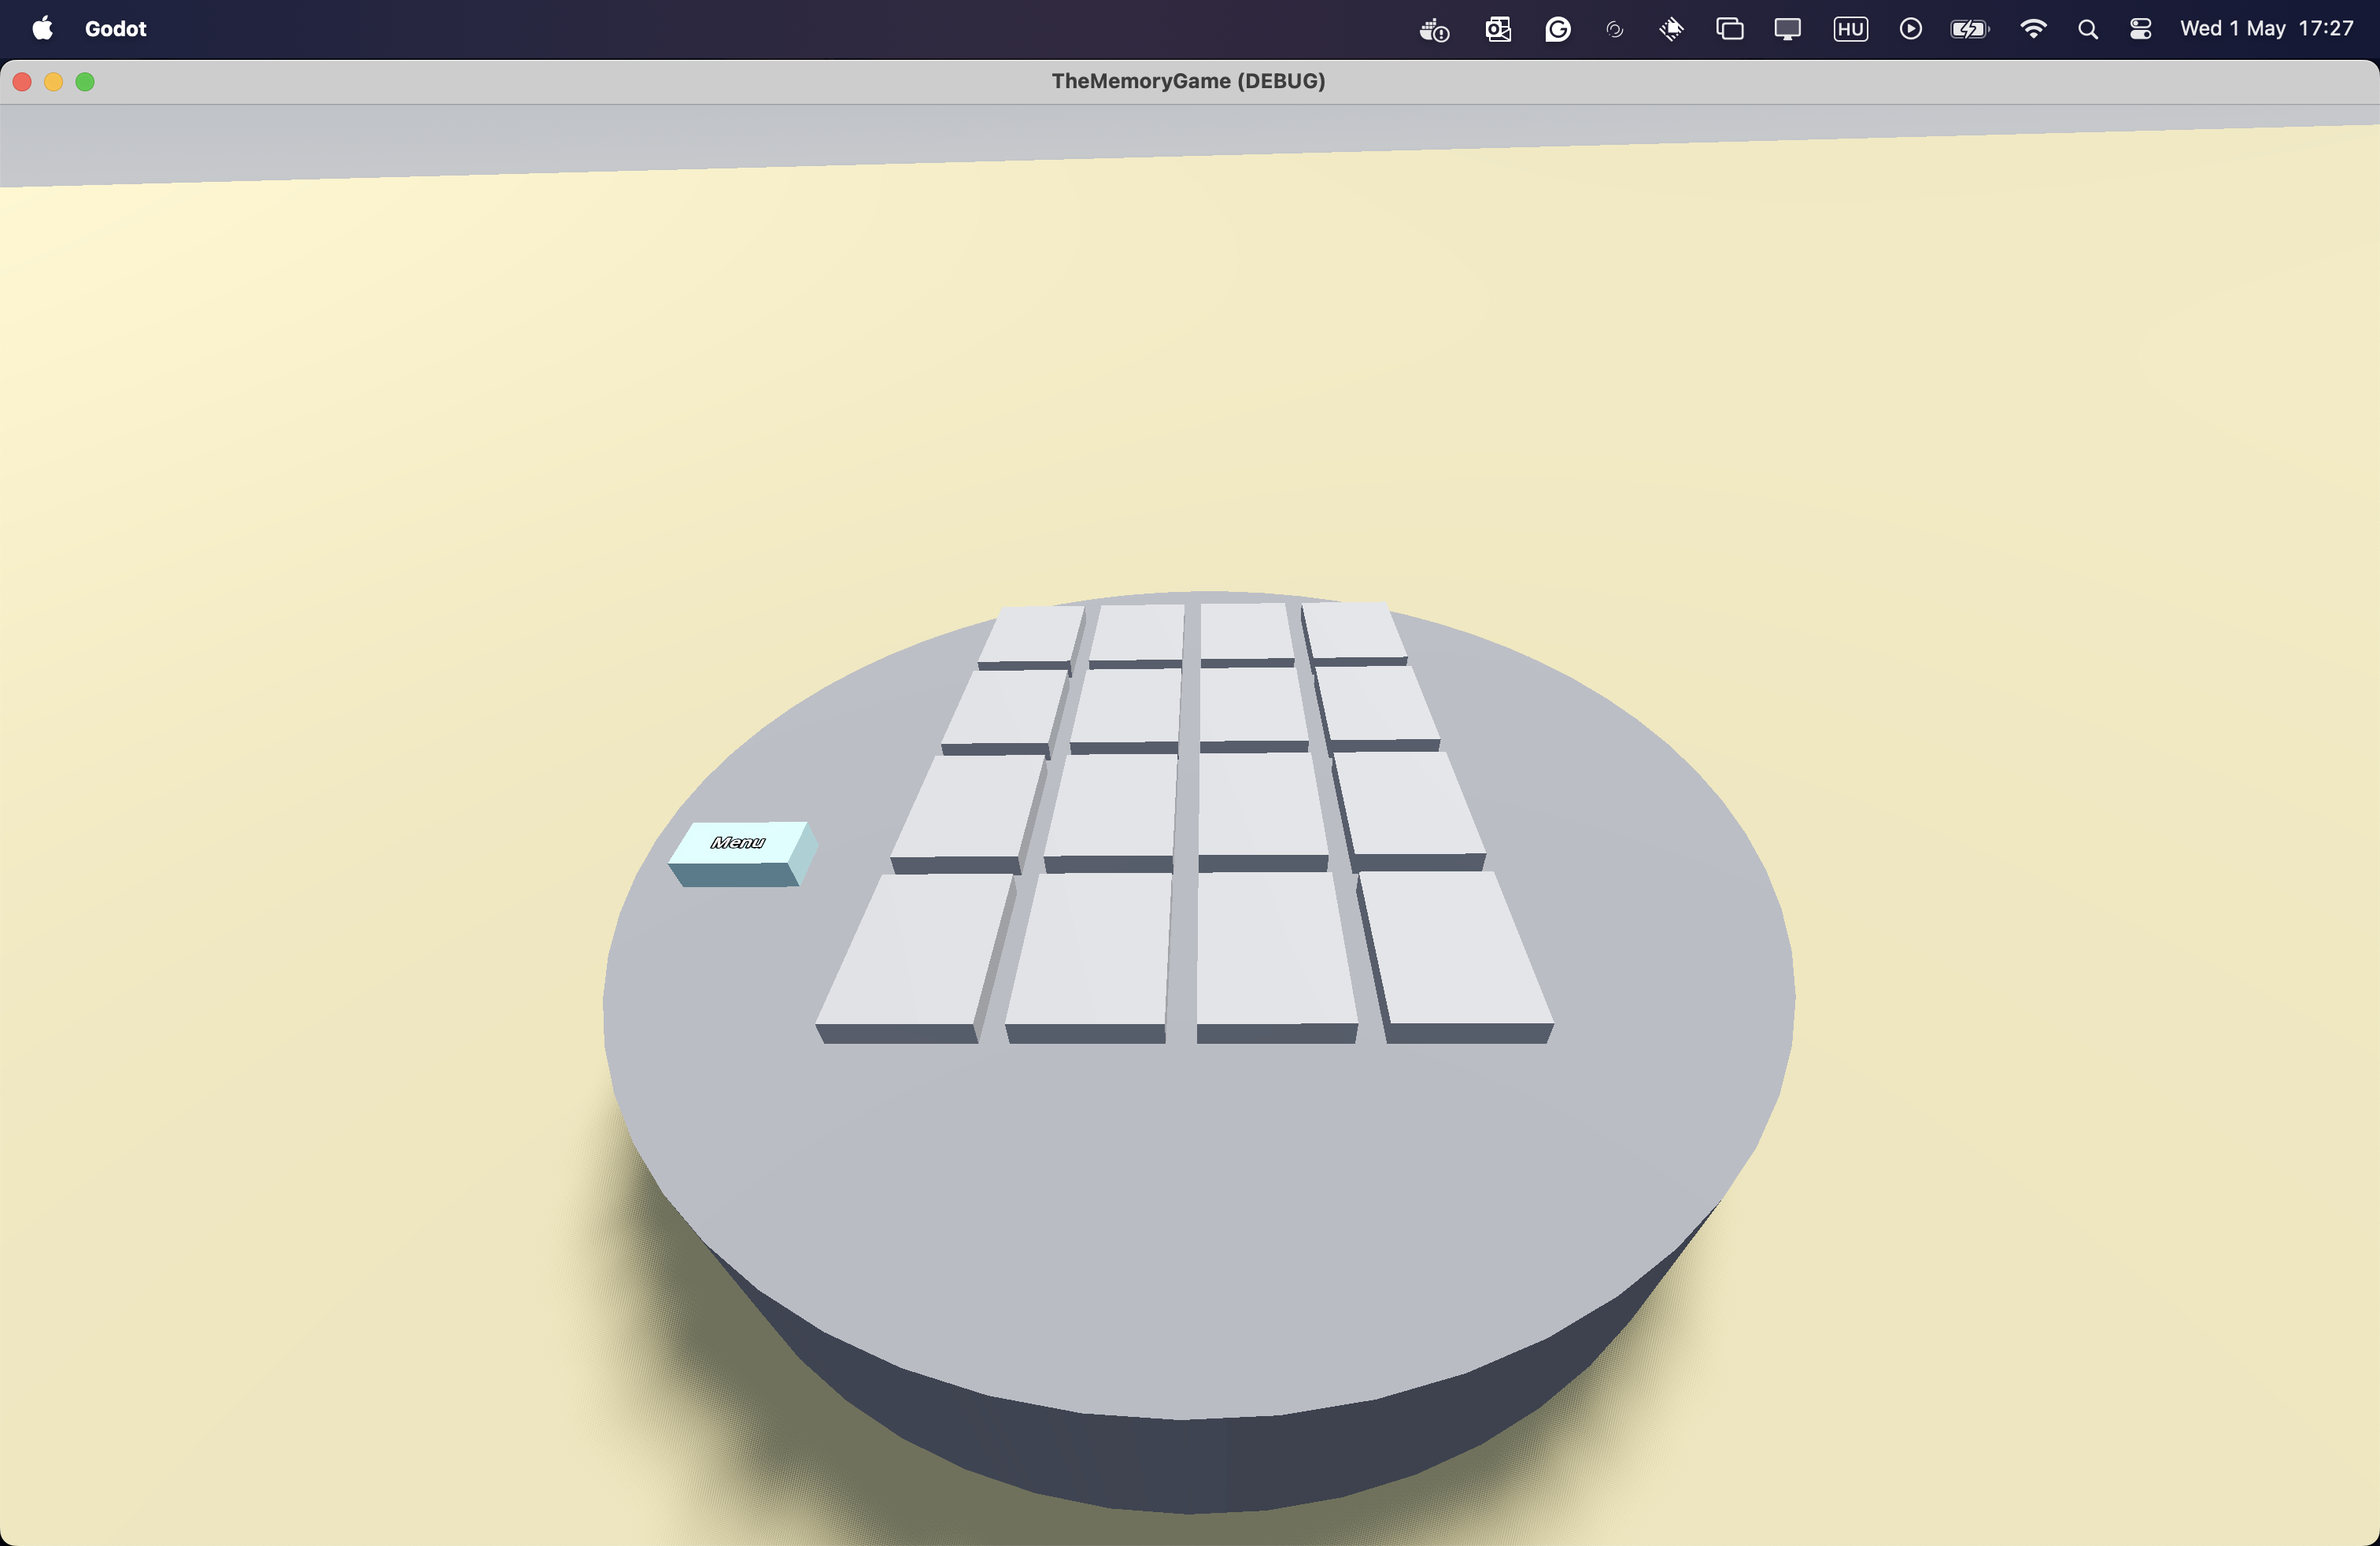
\includegraphics[width=\textwidth]{img/asztal_4x4.png}
    \caption{4x4-es memóriajáték kezdő állapota}
    \label{img:asztal}
\end{figure}
A kártyák előlapján betűk találhatók. Egyjátékos esetben a játékos célja, hogy minél kevesebb kártyapár megfordításából megtalálja az összes memória párt. Többjátékos esetben, hogy ő szerezze a legtöbb pontot, vagyis több kártyapárt fordítson fel, mint az ellenfelei.


Ahhoz, hogy egy kártyát megfordítson, a játékosnak rá kell kattintania. Ekkor láthatóvá válik, mely betűhöz tartozik a memória elemhez (\ref{img:kartya_fliped}. ábra). 
A megfordított kártyához választani kell egy másikat. A játékosnak törekednie kell, hogy korábbi ismeretei alapján, a következőre a választott kártya előlapján ugyanaz a betű szerepeljen, mint a már felfordított memória lapon, vagyis egy párt fordítson fel. 
Értelemszerűen ez az első felfordításkor nem lehetséges, hiszen nincs korábbi ismerete a játékról (\ref{img:non_pair}. ábra).
\begin{figure}[h]
\begin{subfigure}[t]{0.5\textwidth}
    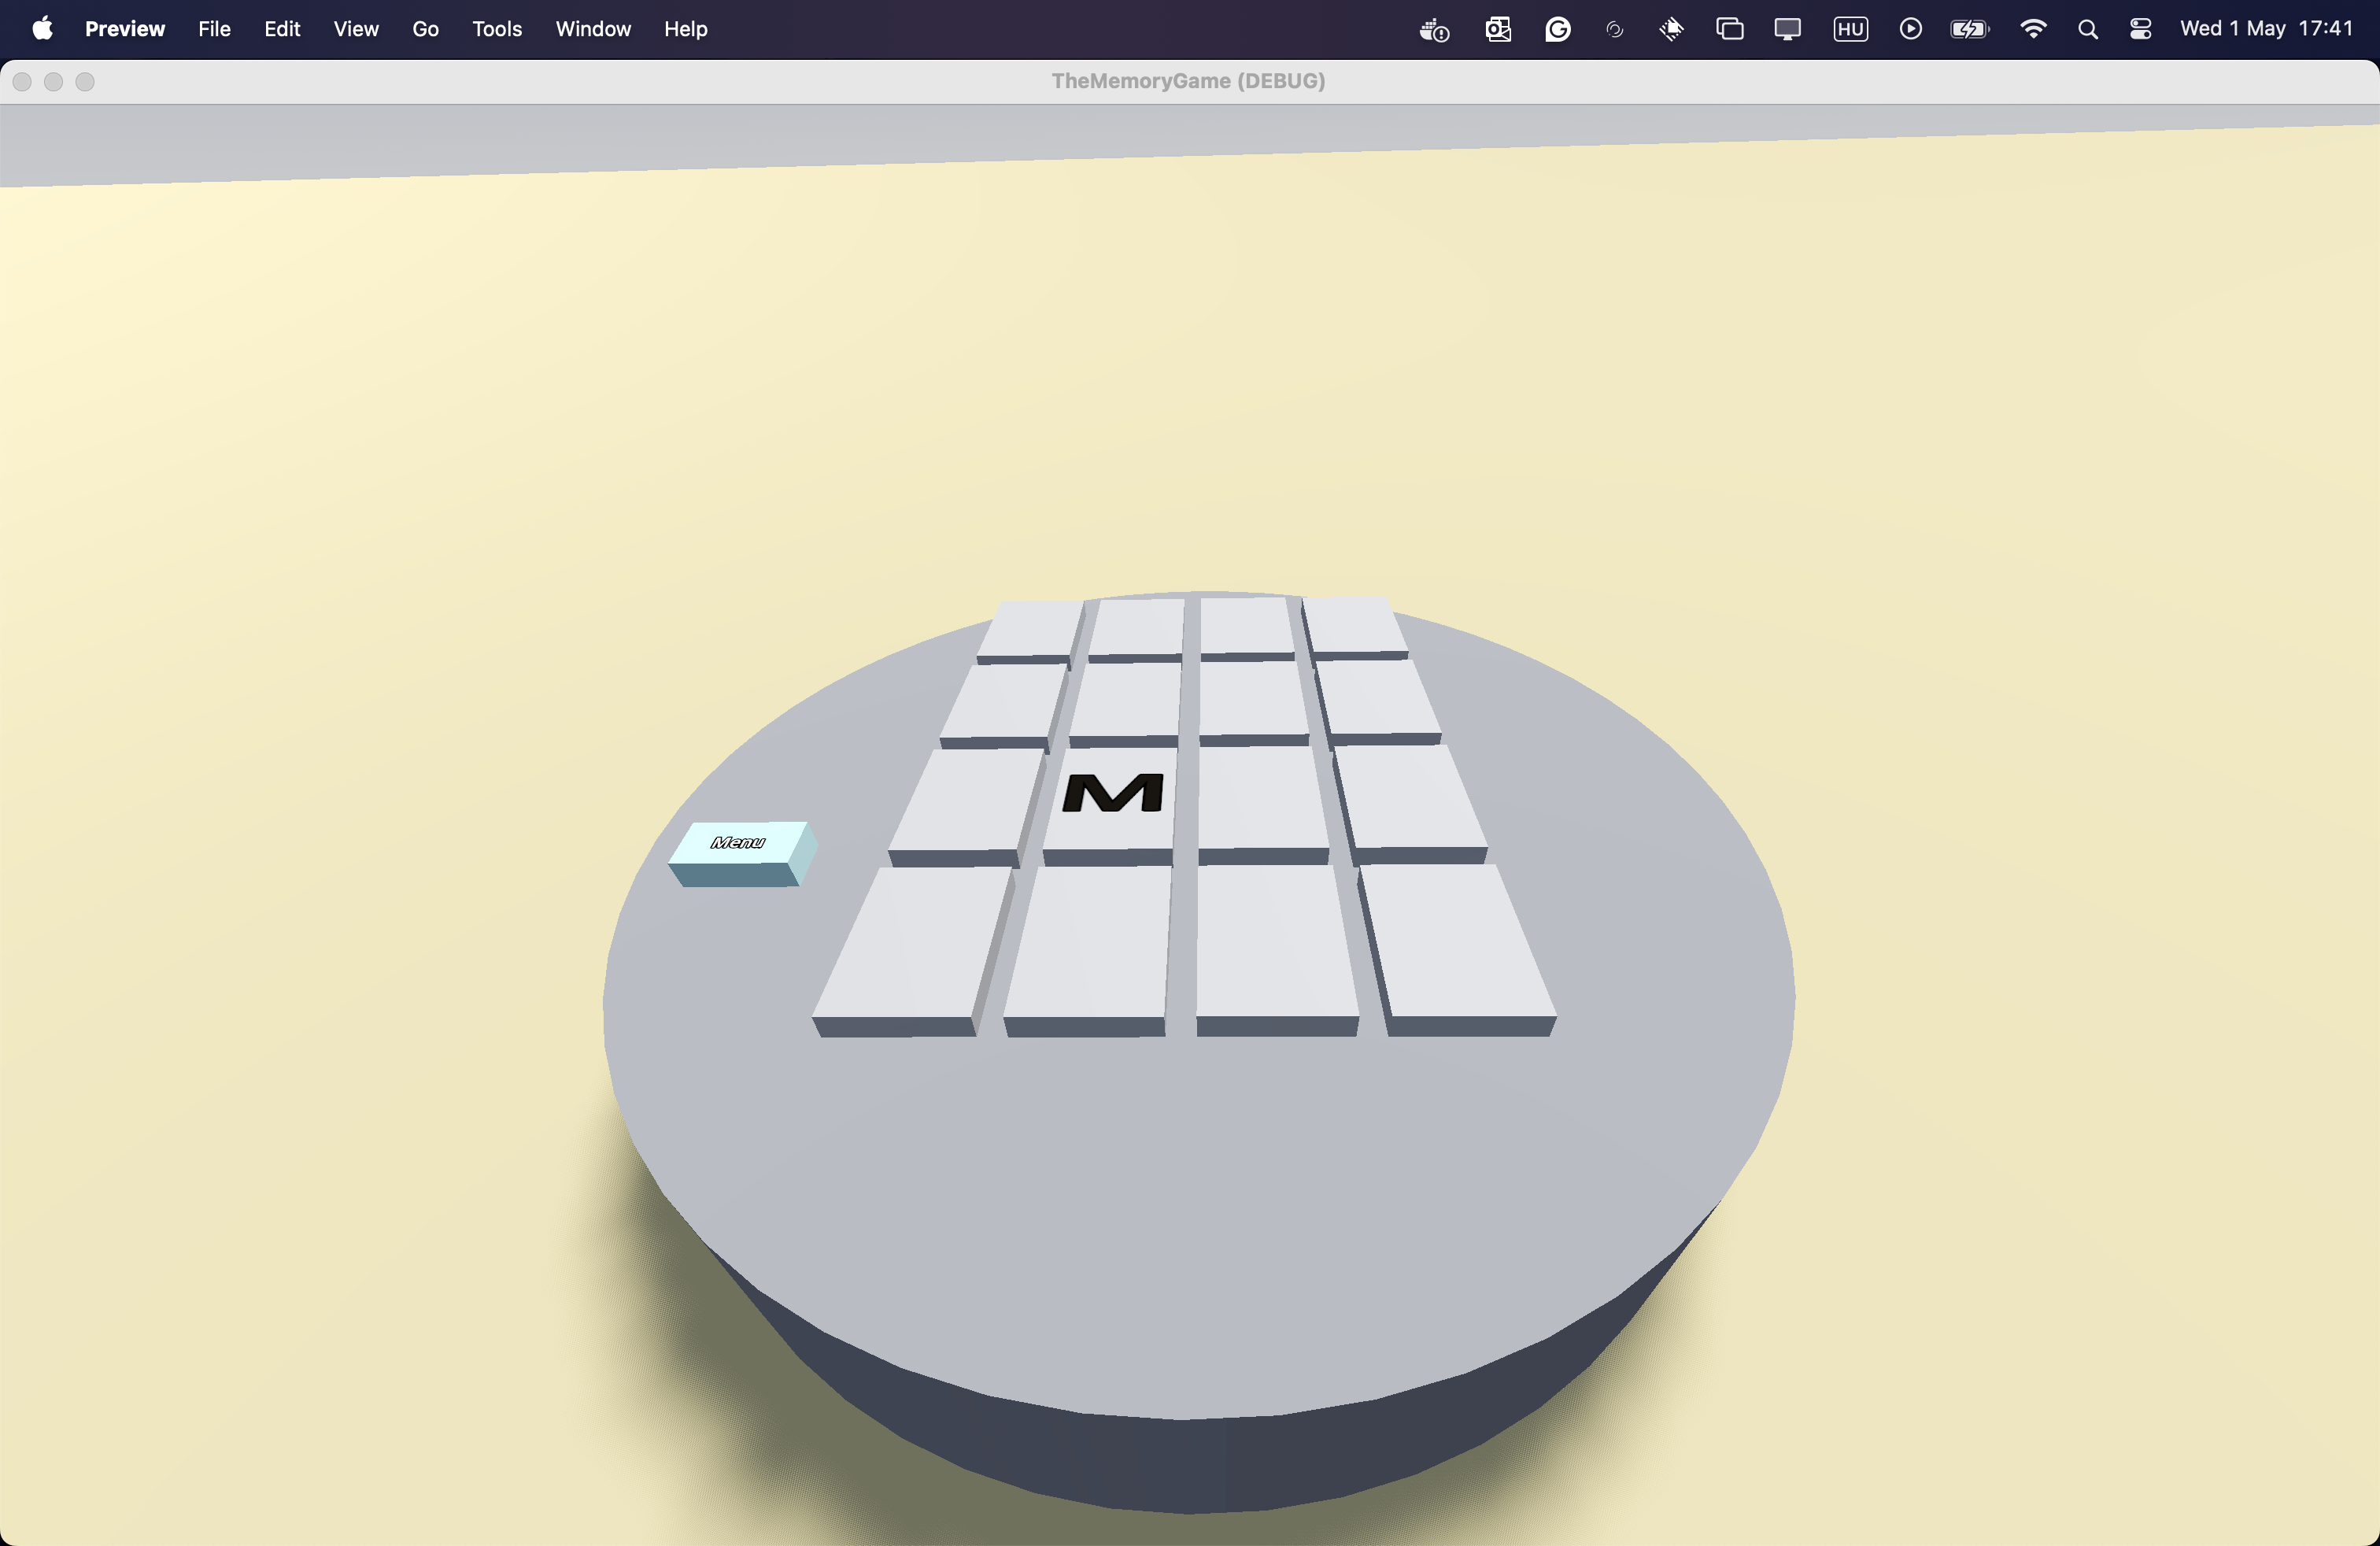
\includegraphics[width=\linewidth]{img/asztal_4x4_card_flipped.png}
    \caption{Egy kártya ki van választva}
    \label{img:kartya_fliped}
\end{subfigure}
\begin{subfigure}[t]{0.5\textwidth}
    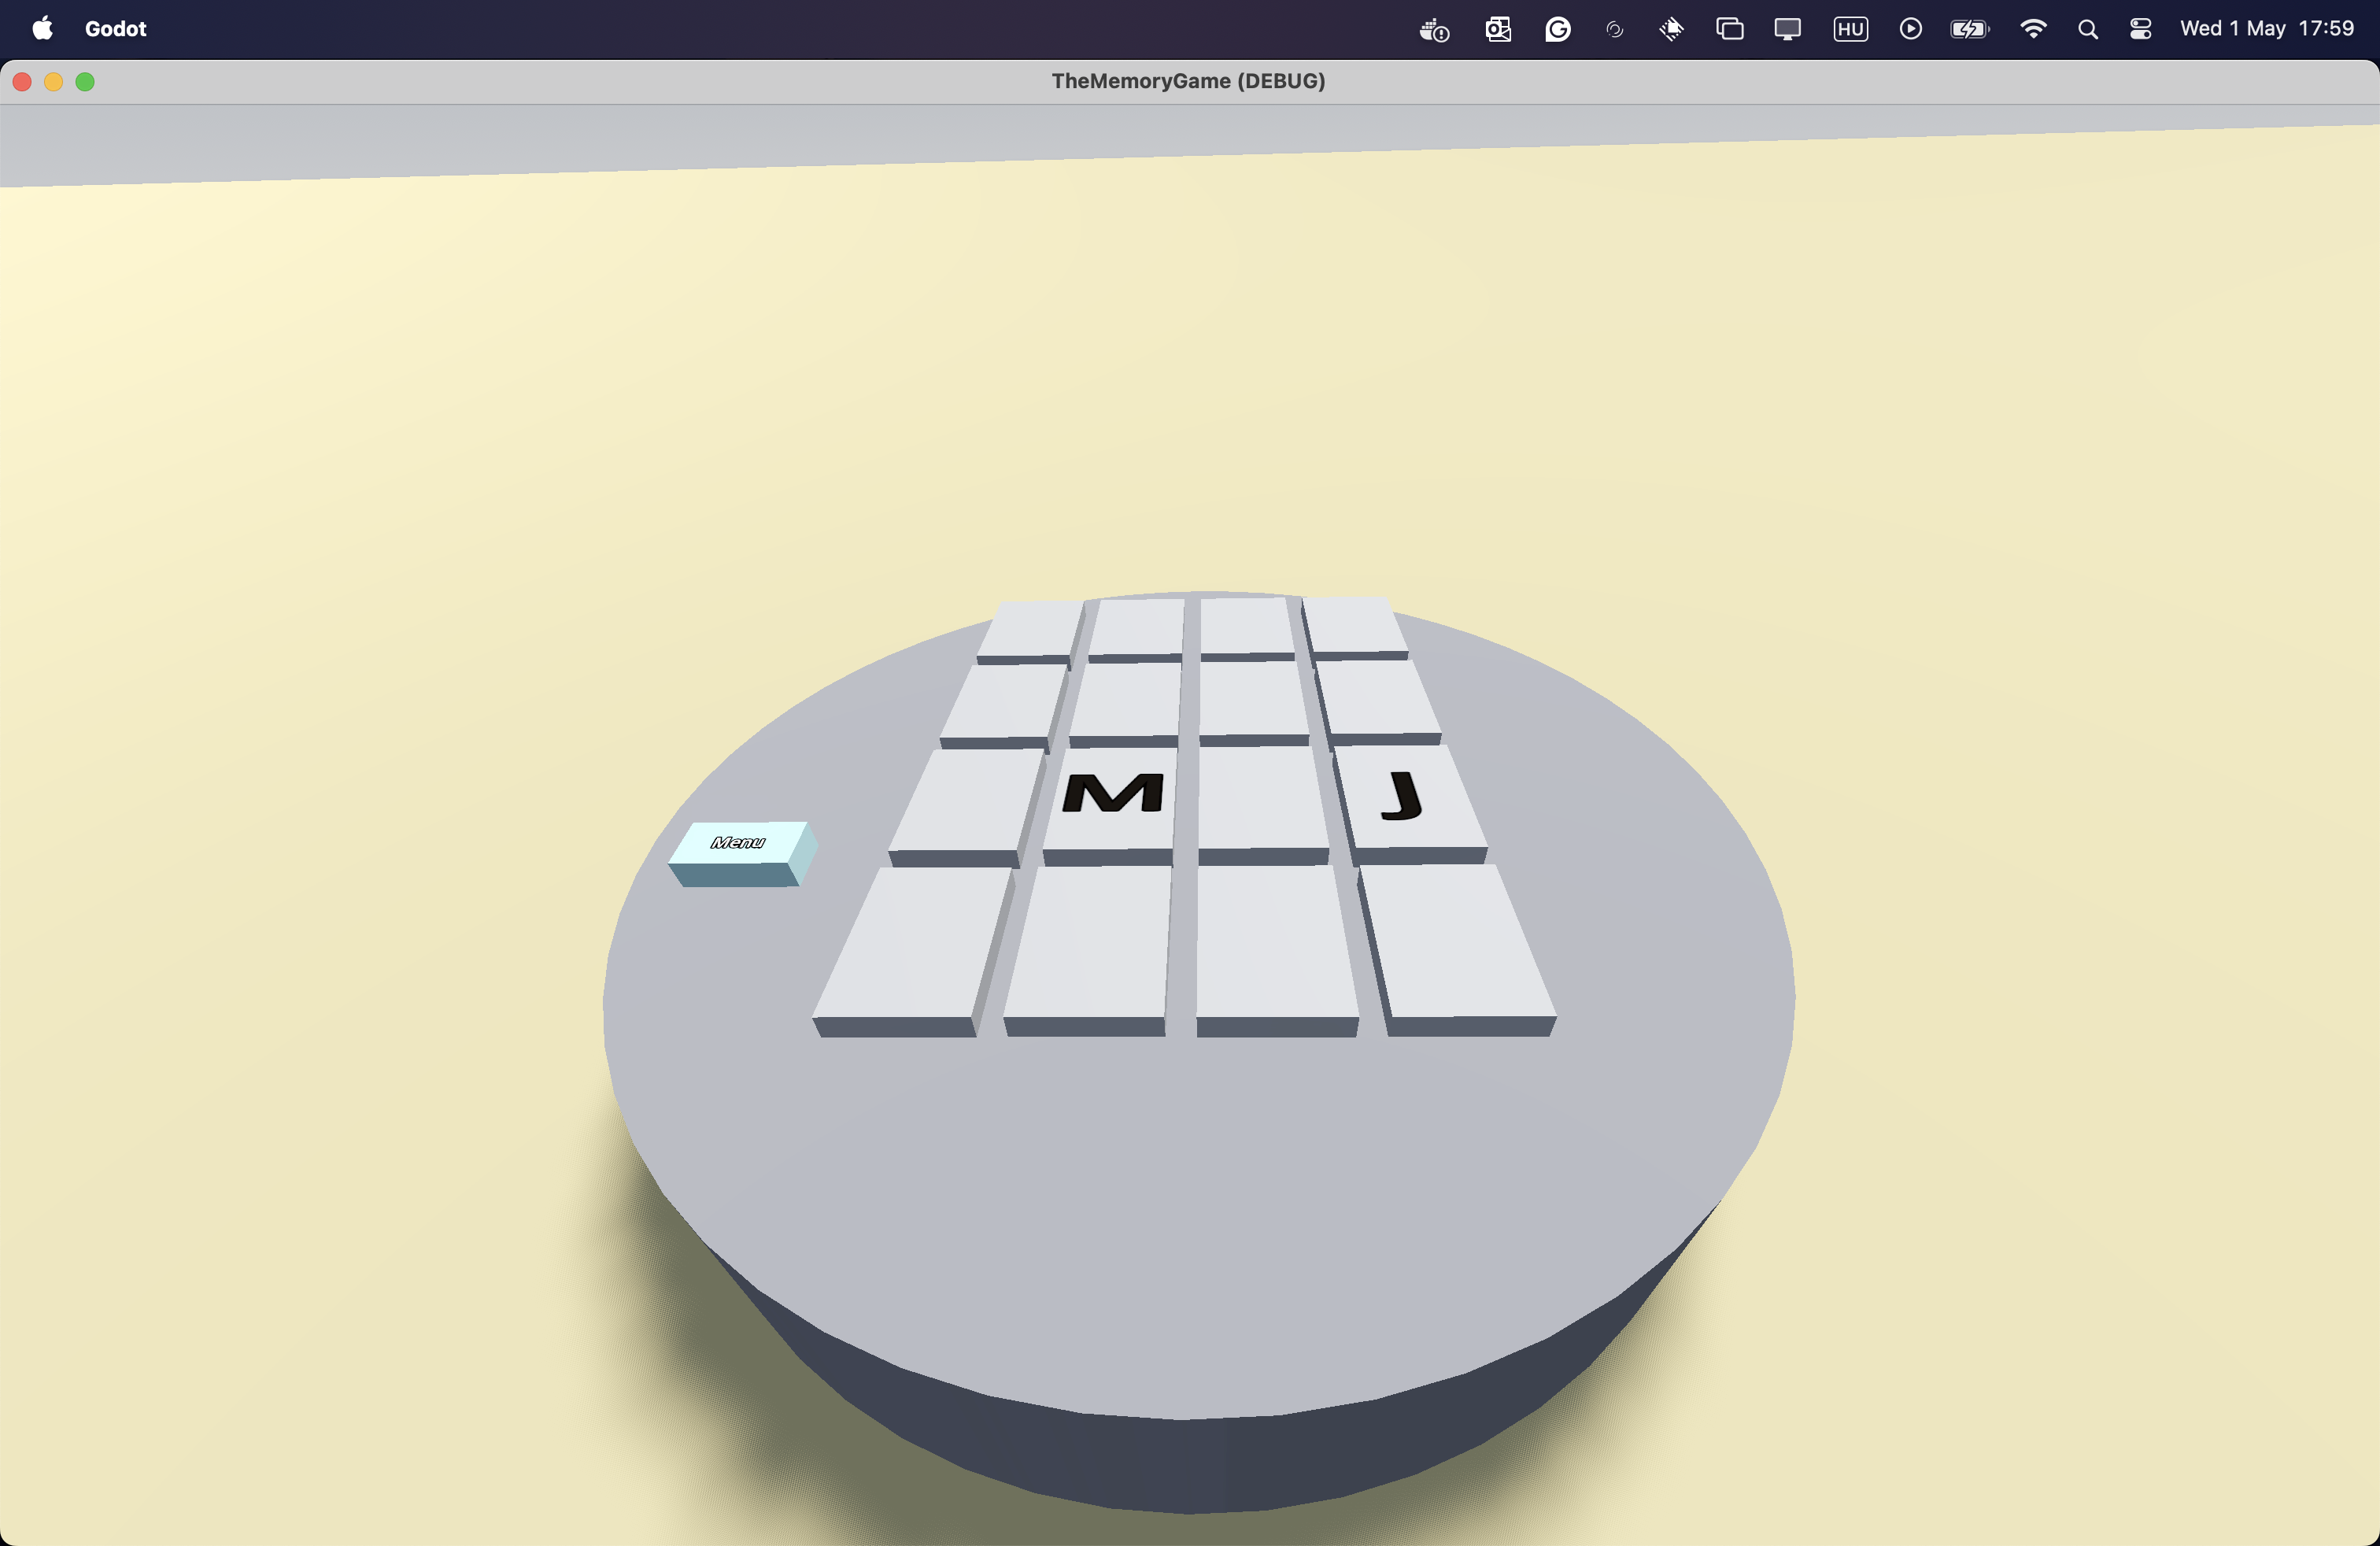
\includegraphics[width=\linewidth]{img/asztal_4x4_non_pair.png}
    \caption{Mivel a betűk nem azonosak, ezér ez nem egy pár, visszafordítjuk a kártyákat.}
    \label{img:non_pair}
\end{subfigure}
\caption{4x4-es játék, példa kör, amikor nem egy párt húzunk fel}
\end{figure}
Ha a felfordított kártyák nem alkotnak párt, akkor a kártyák maguktól visszafordulnak pár másodperc elteltével. Ez után egyszemélyes játék esetén esetén végrehajtunk egy újabb fordítást. Többjátékos esetén a következő játékos végezheti el a körét. 

Ha párt alkotnak (\ref{img:pair}. ábra), akkor a kártyák eltűnnek a játékmezőről  (\ref{img:pair_gone}. ábra).Többjátékos esetben a felfordított játékos kap egy pontot, és egy újabb fordítással folytatja a körét, mindaddig, míg egy nem párt fordít.
\begin{figure}[H]
    \begin{subfigure}[ct]{0.5\textwidth}
        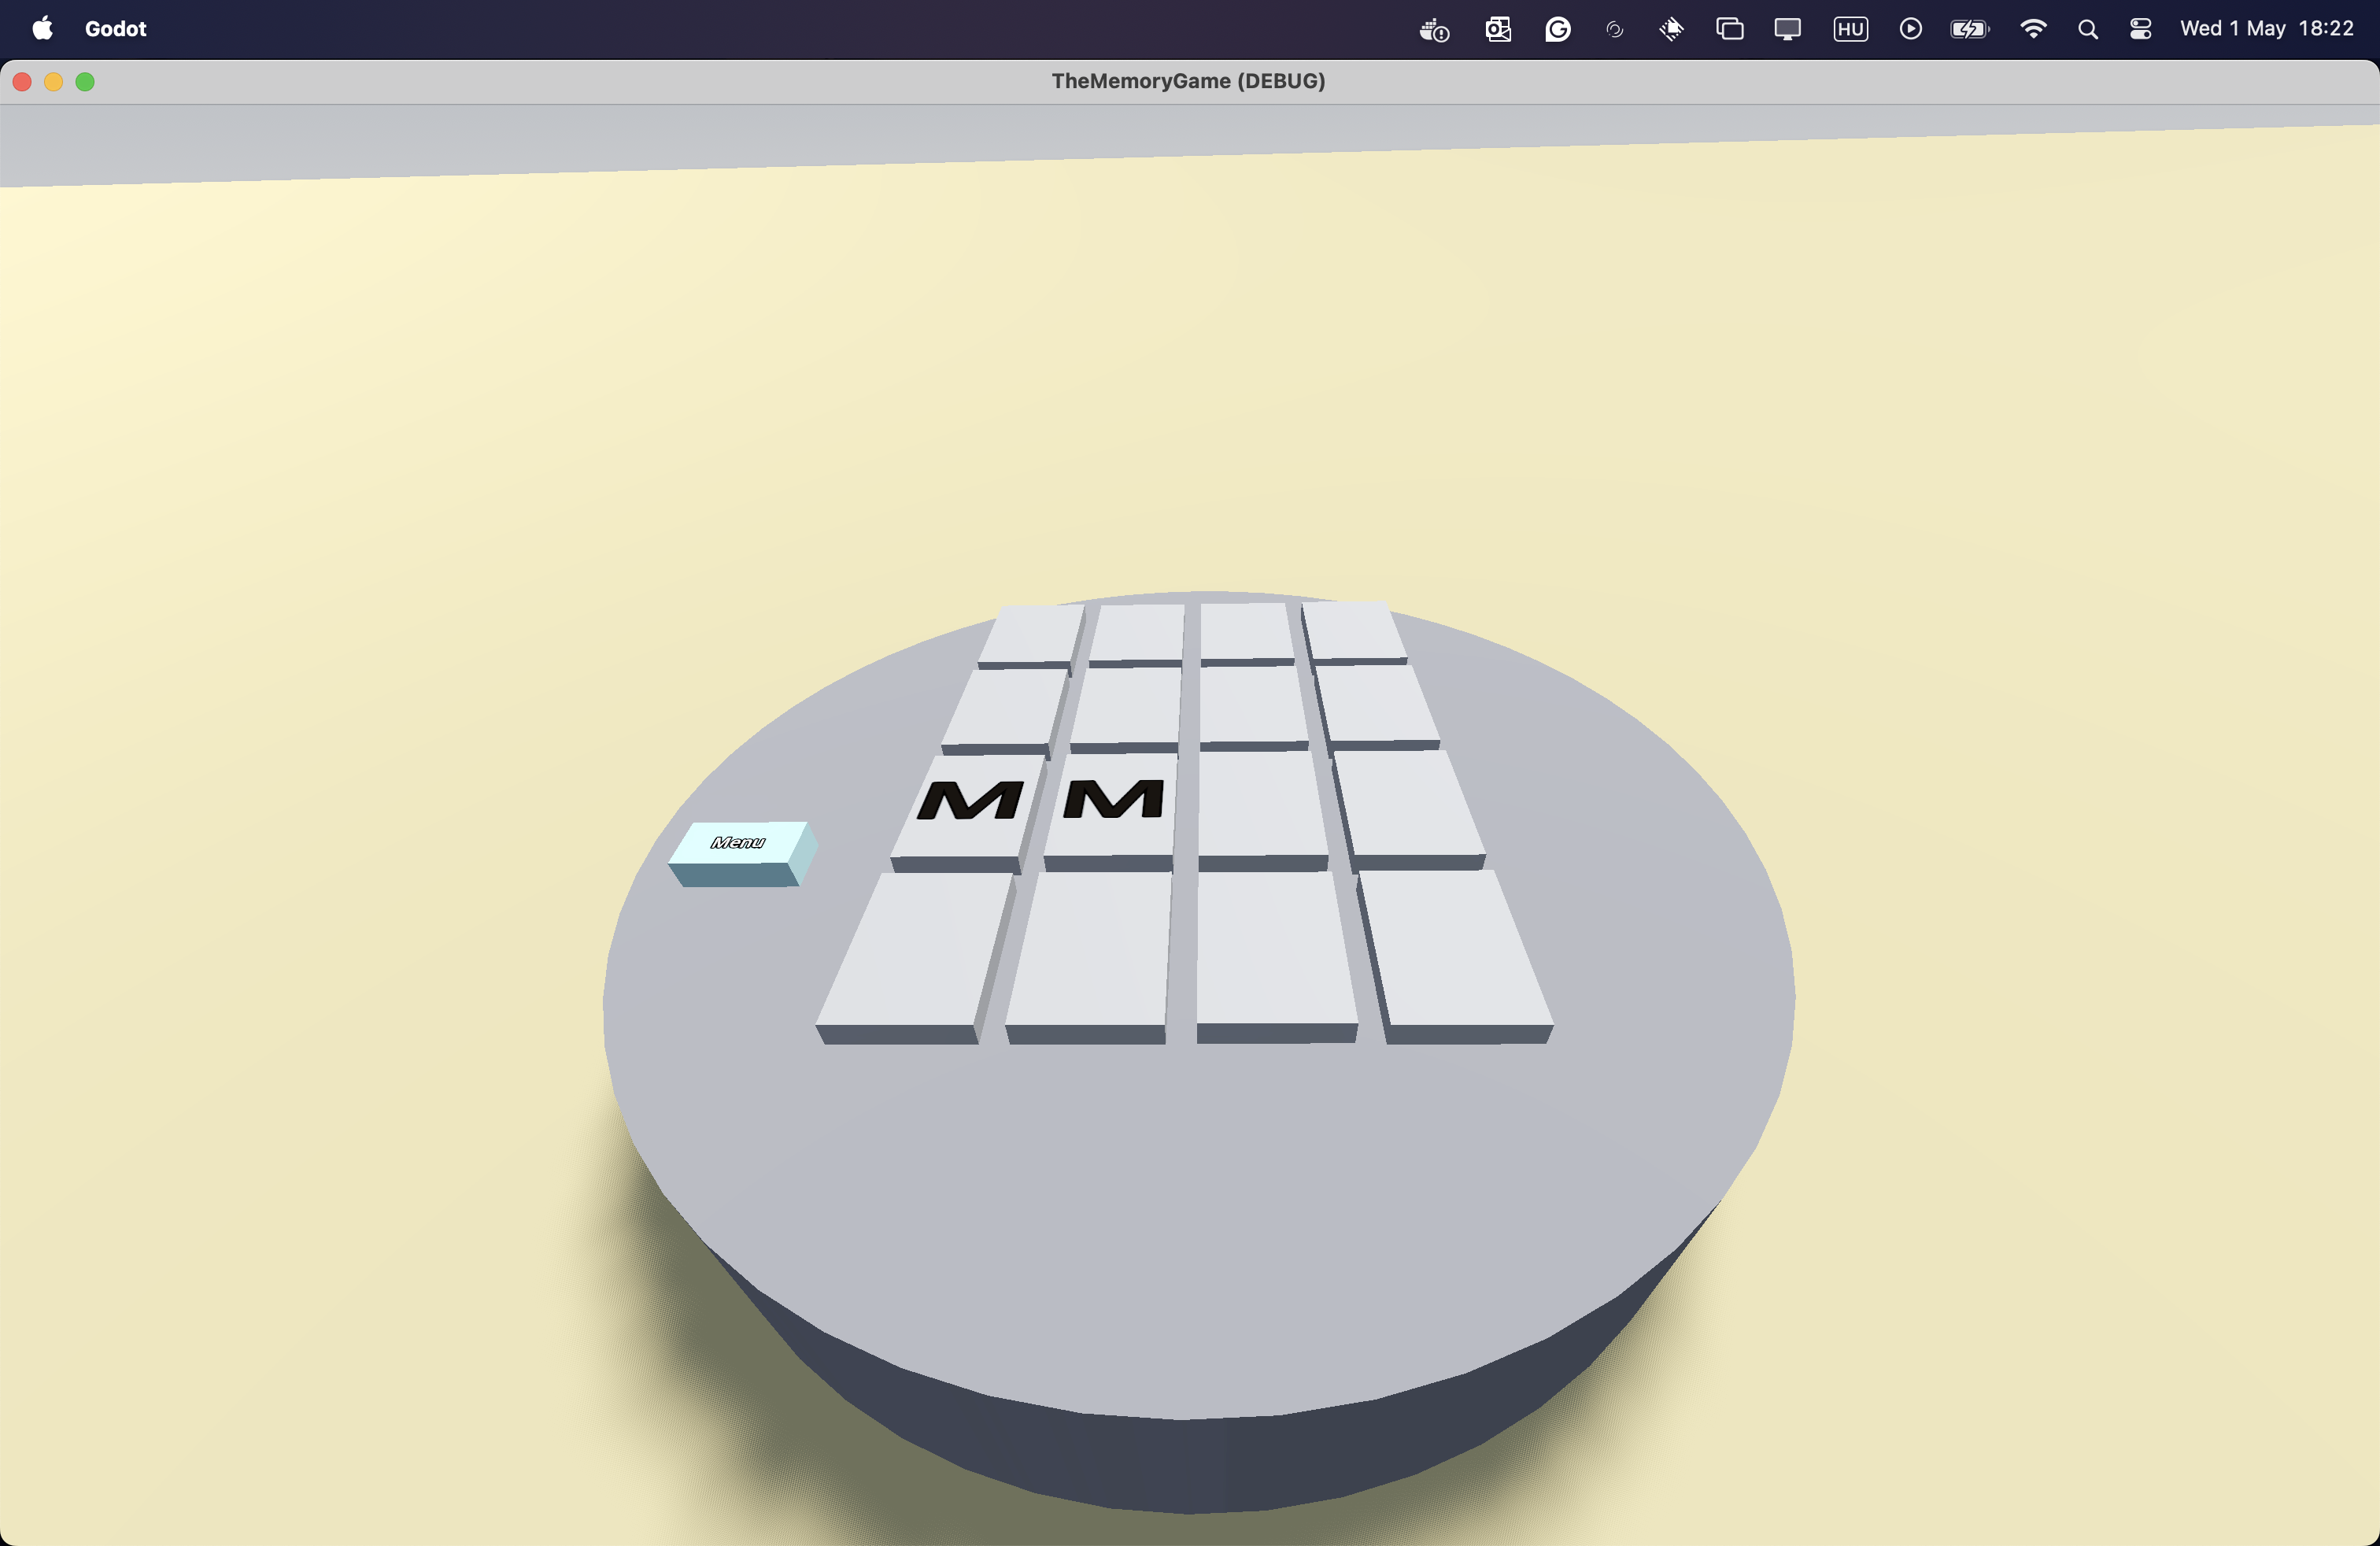
\includegraphics[width=\textwidth]{img/asztal_4x4_pair.png}
        \caption{A kiválasztott kártyák párt alkotnak}
        \label{img:pair}
    \end{subfigure}
    \begin{subfigure}[ct]{0.5\textwidth}
        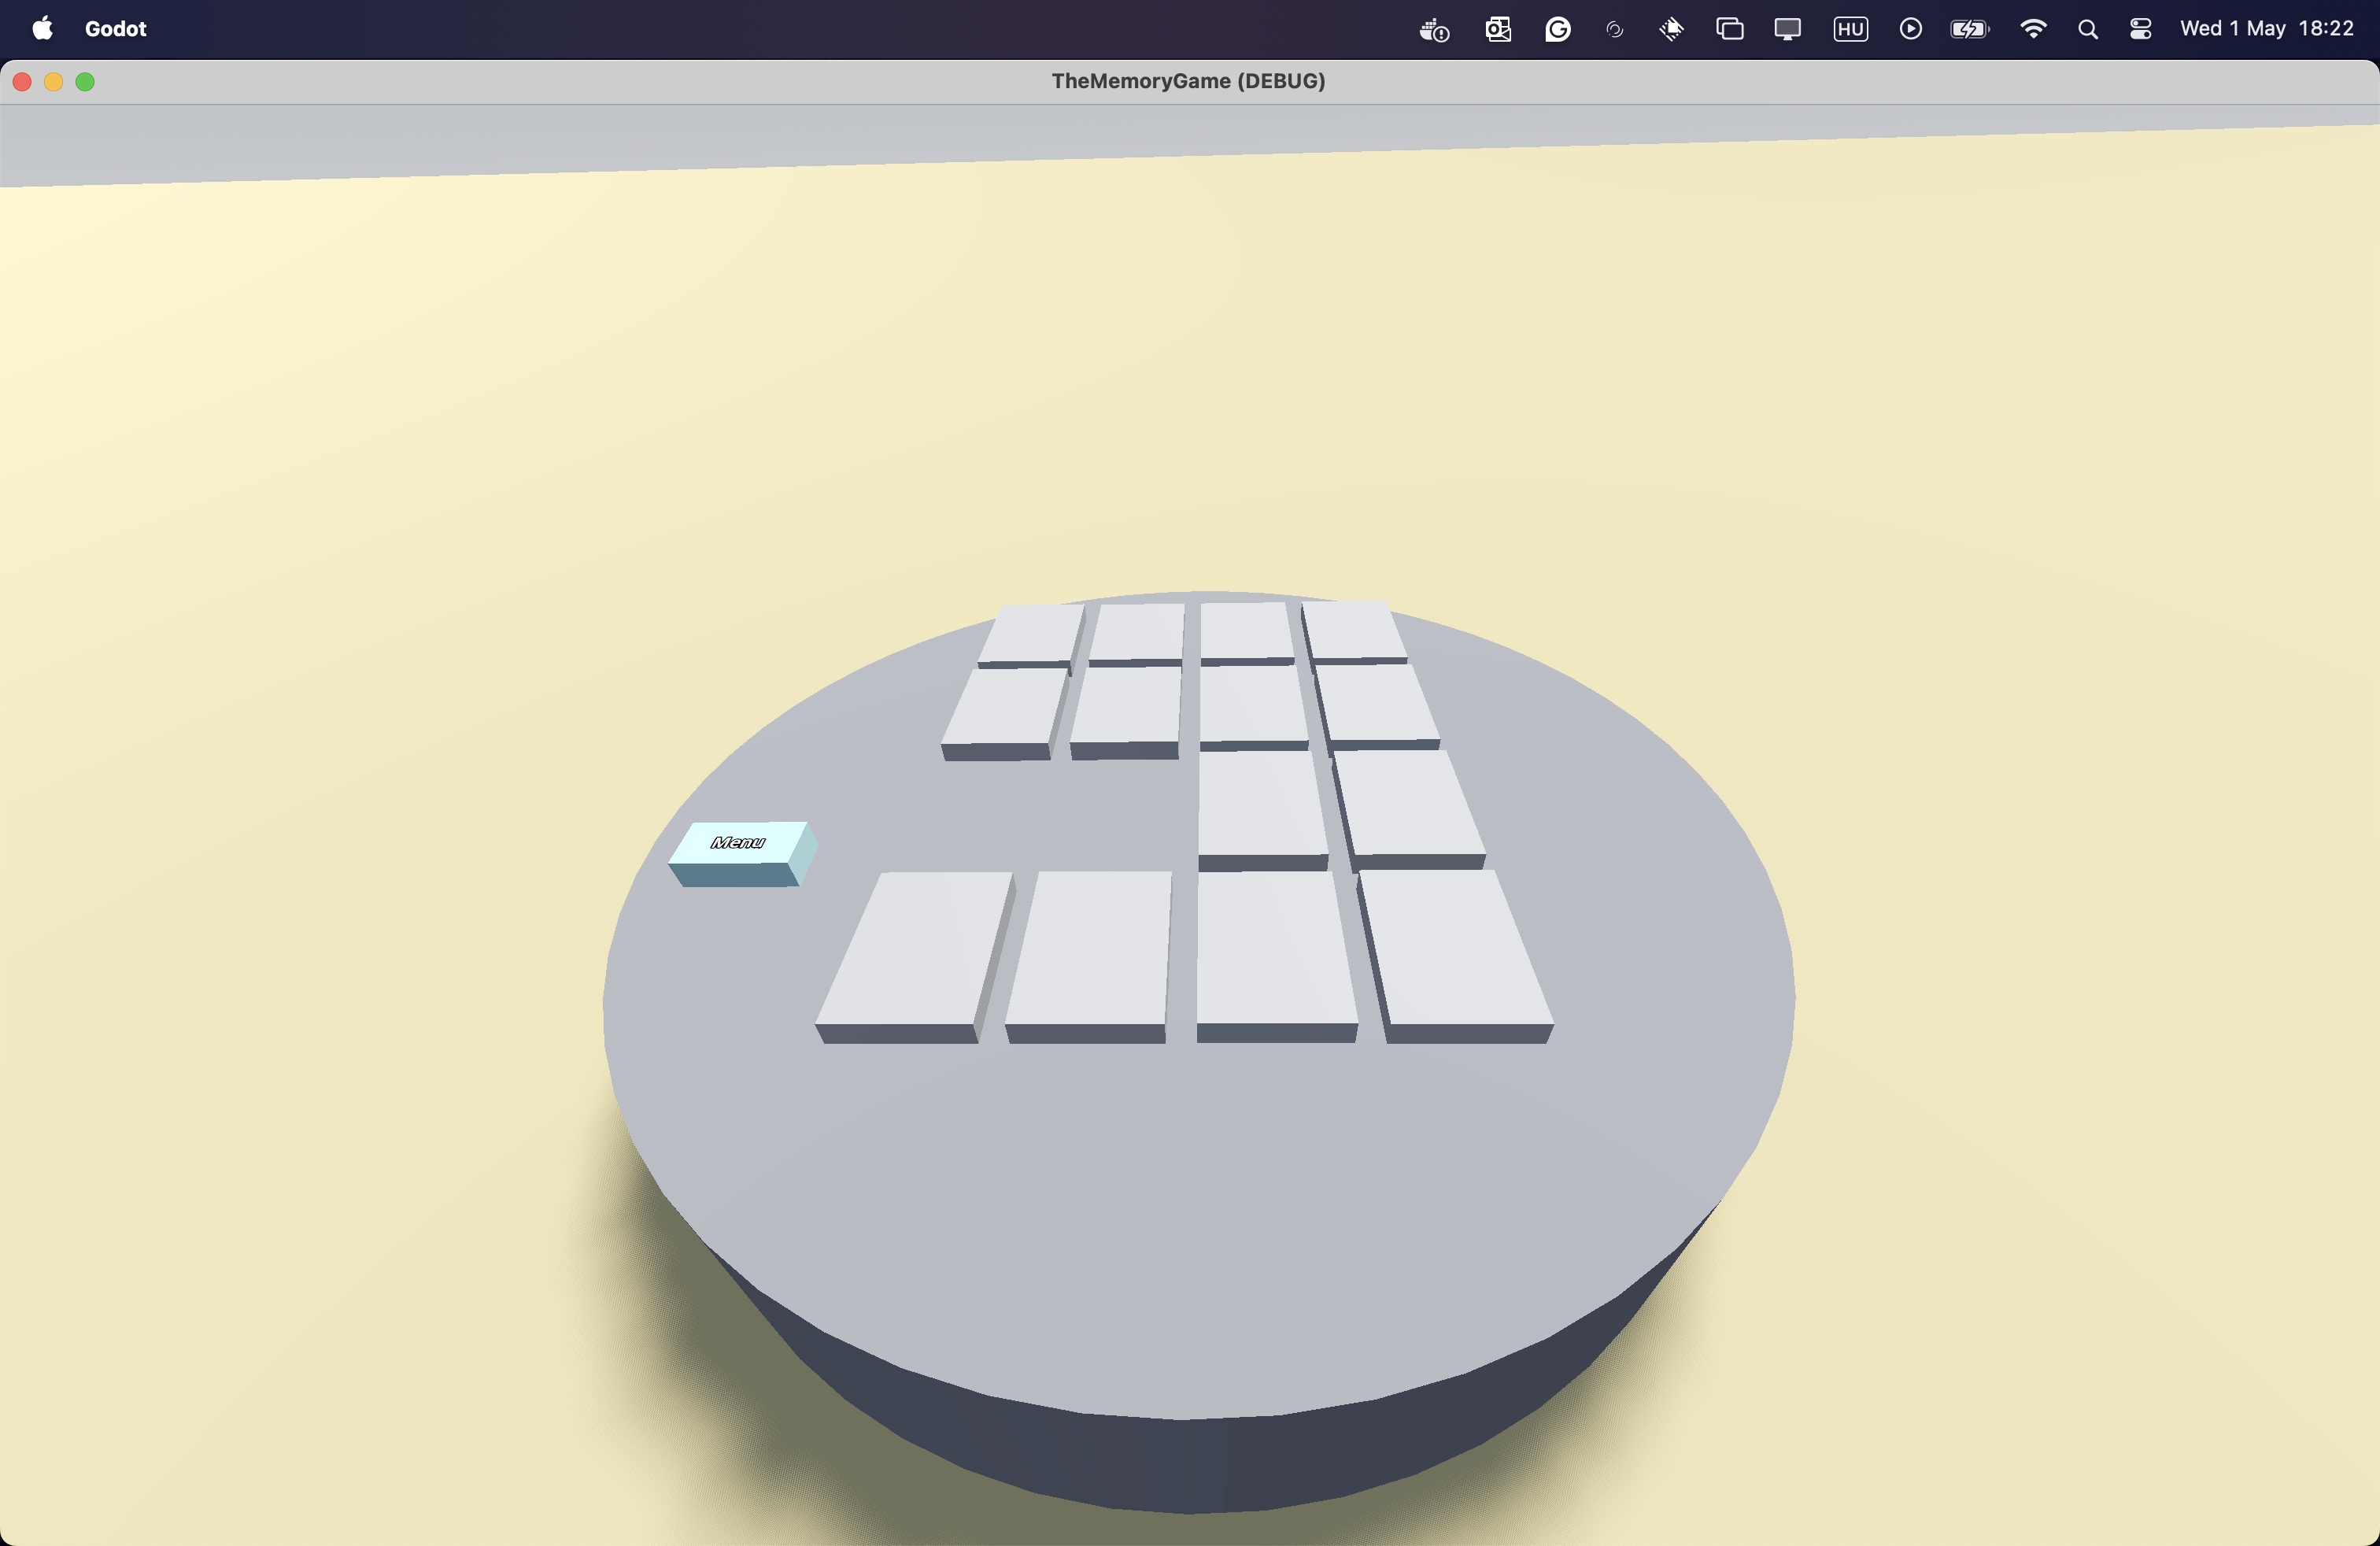
\includegraphics[width=\textwidth]{img/asztal_4x4_pair_eltunik.png}
        \caption{Eltűnik a pár az asztalról}
        \label{img:pair_gone}
    \end{subfigure}
    \caption{4x4-es játék, példa kör, amikor egy párt húzunk fel}
\end{figure}


Amint az összes kártya eltűnik az asztalról, a játék véget ér, és visszakerülünk a menübe.
A játékba több nehézségi szintet tettünk, melyet a menüből érhetünk el (\ref{img:menu}. ábra). A különböző menüpontok, a kártyák számának elhelyezkedését jelölik.
\begin{figure}[h]
    \centering
    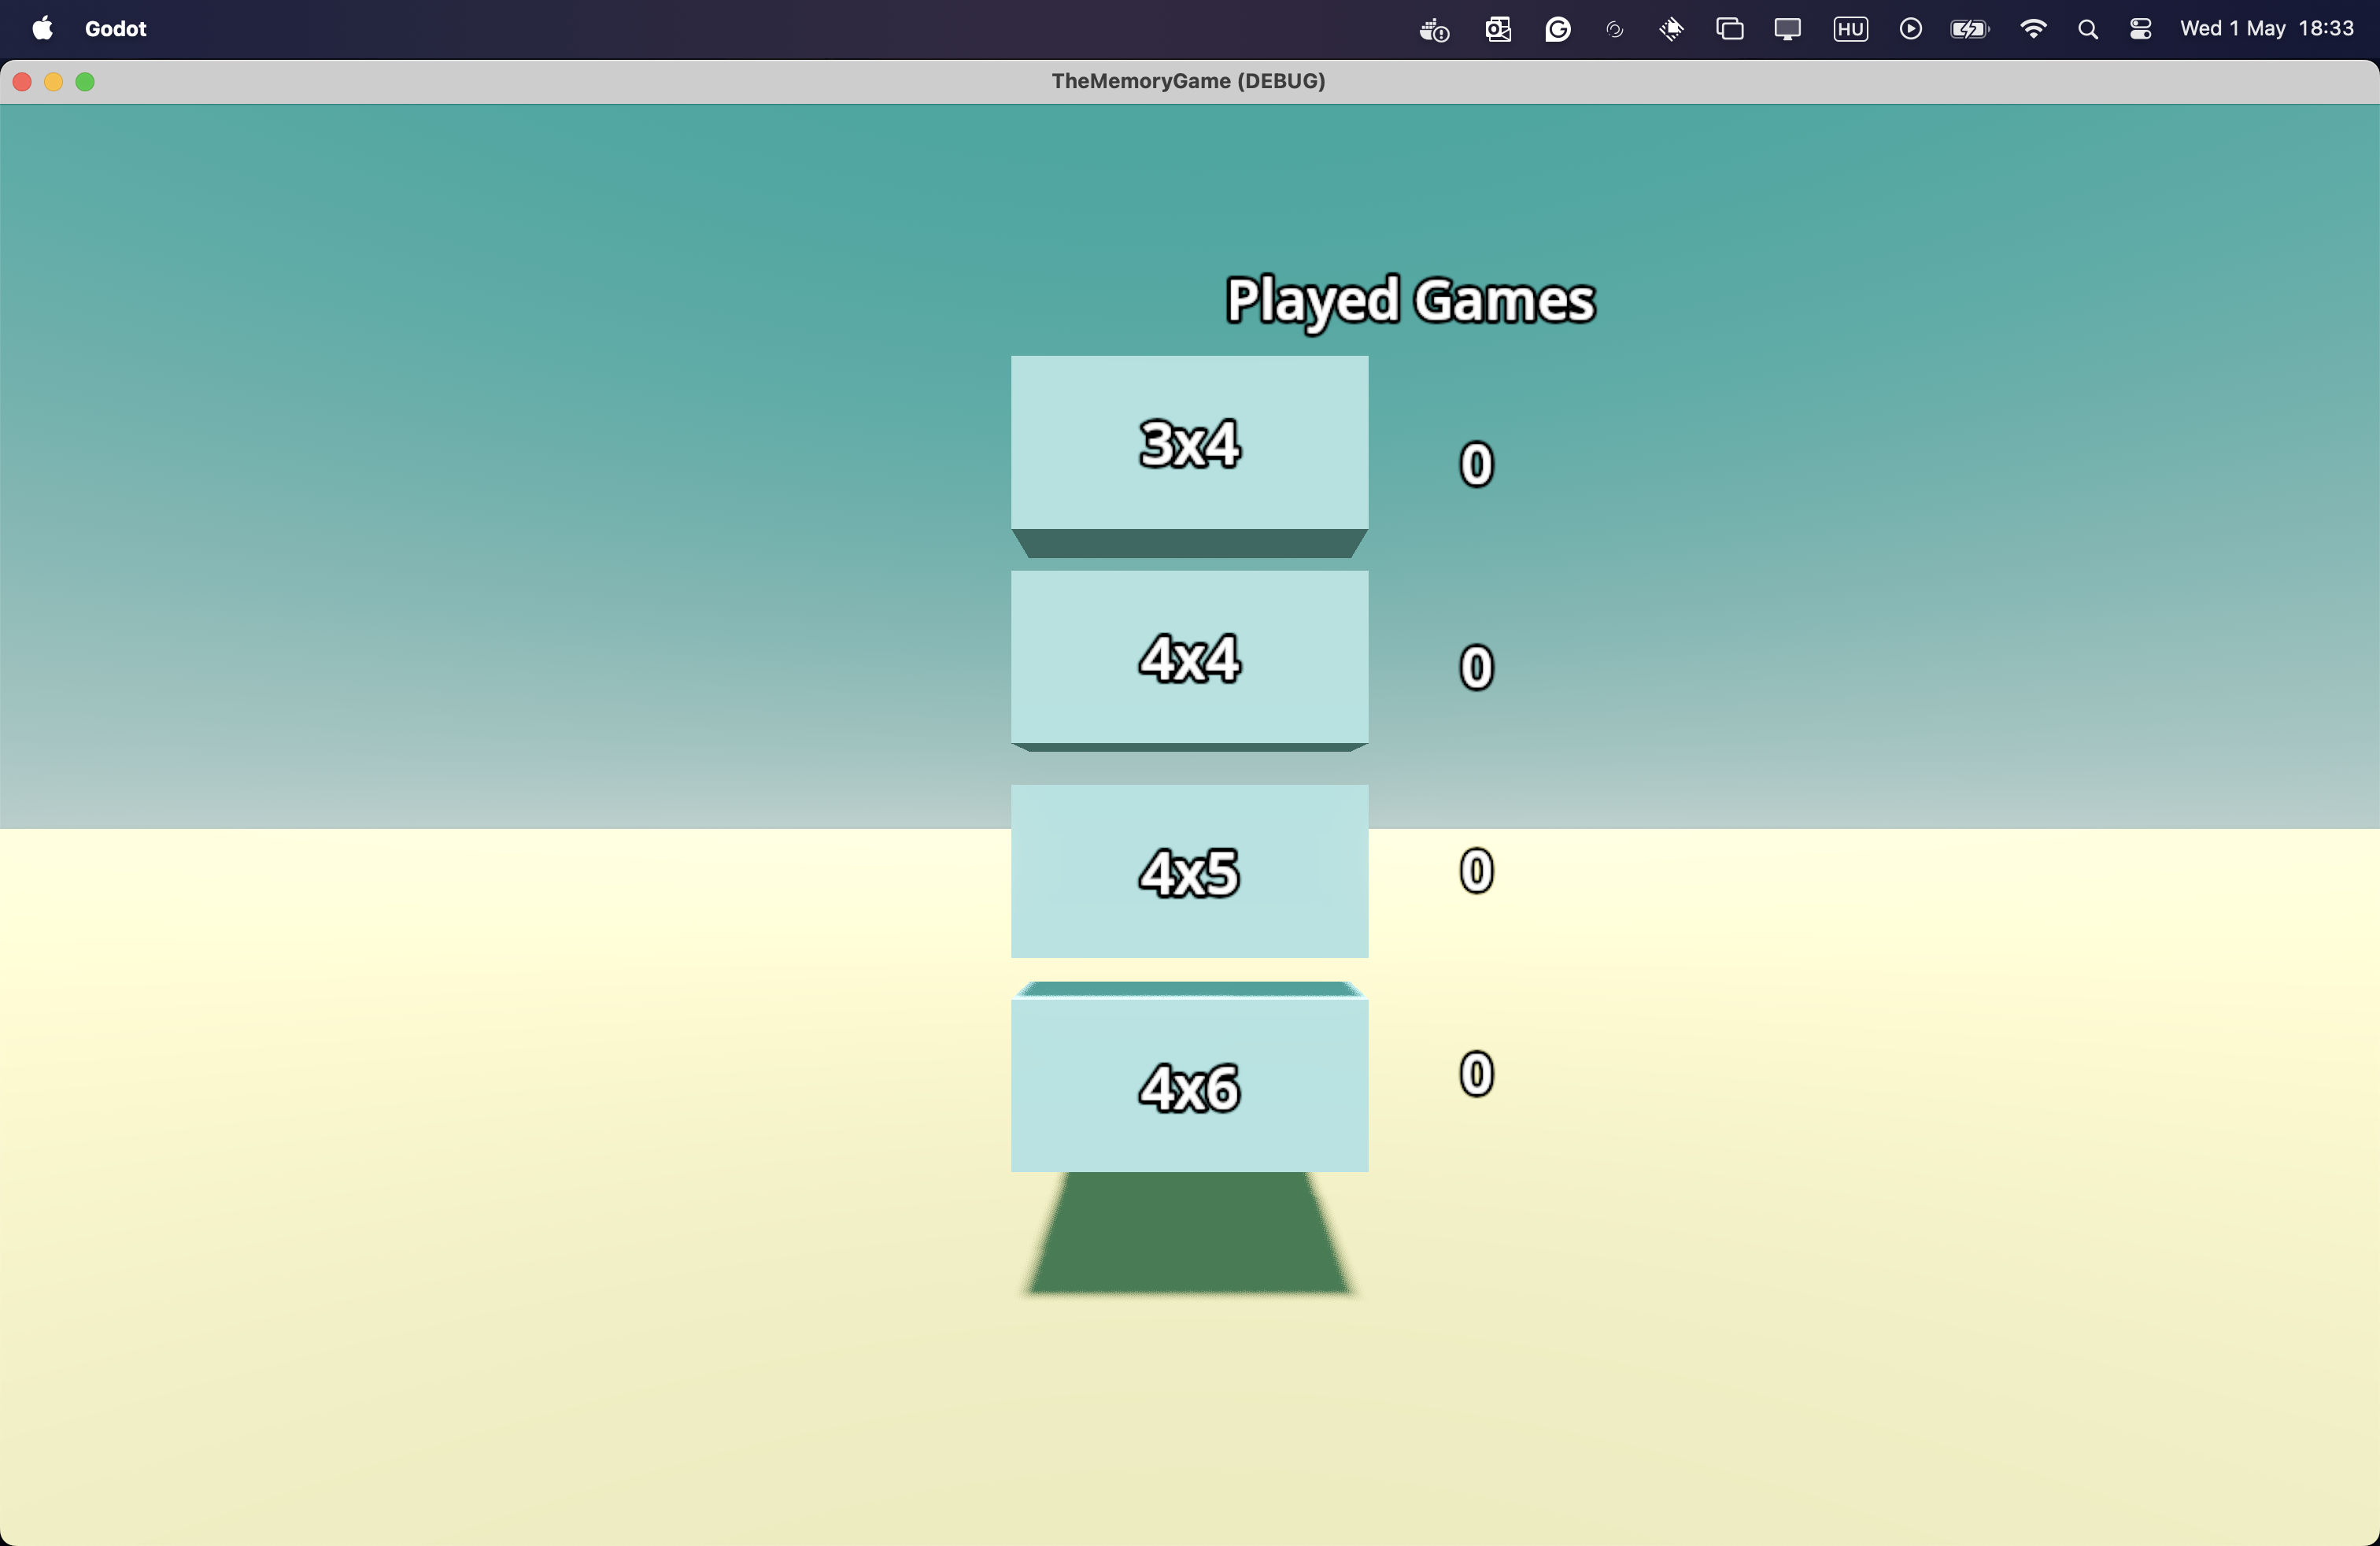
\includegraphics[width=0.5\textwidth]{img/menu.png}
    \caption{A játék menüje}
    \label{img:menu}  
\end{figure}

\section{Struktúrális felépítés}
A memória játék a Godot elveinek megfelelően Node-okból és Scene-ekből \cite{godotengineNodesScenes} áll. A Scene-ek struktúrája a következő.
\subsection{Menü}


A Játék menüje (\ref{img:menu_scene}. ábra), a következő módon épül fel. A Gombok olyan MeshInstance3D Node-ok \cite{godotengineMeshInstance3D}, melyekre ha a játékos rákattint, akkor emittálnak egy \lstinline{button_pressed()} signal-t (\ref{code:button_pressed_signal}. ábra).
A MenuScene kódjában hallgatózunk erre külön külön a gombokra. A megfelelő gomb megnyomásával beállítjuk a \lstinline{Constant.CARD_PAIR_NUMBER} globális változót, mely segítségével létrehozzuk a \lstinline{basic_scene}-t.
\begin{figure}[h]
    \centering
    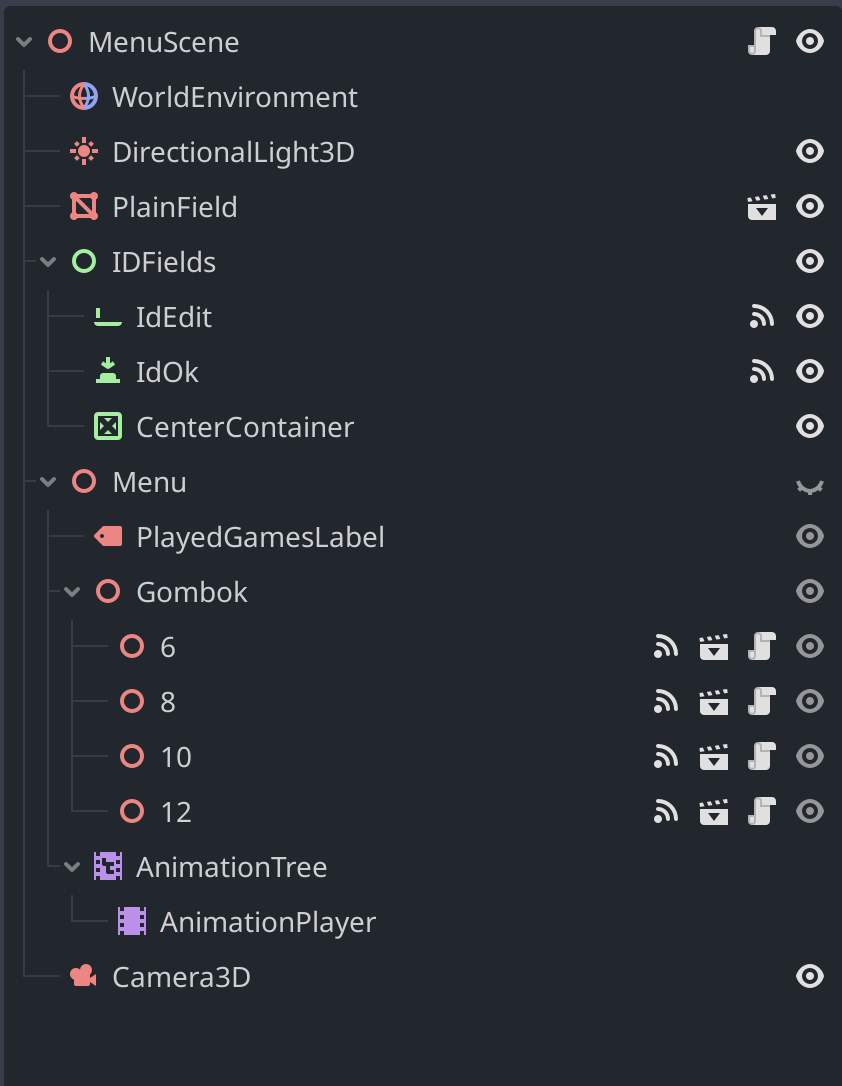
\includegraphics[width=0.5\textwidth]{img/menu_scene_tree.png}
    \caption{A játék menü Scene-jének struktúrája}
    \label{img:menu_scene}  
\end{figure}

\begin{figure}[H]
    \centering
    \begin{lstlisting}[language=GDScript]
    func _on_area_3d_input_event(camera, event, position, normal, shape_idx):
        if event is InputEventMouseButton:
            if (event.button_index == MOUSE_BUTTON_LEFT && event.pressed == true):
                emit_signal("button_pressed")
    
    func set_number_label_text(new_label_text: String):
        number_label.text = new_label_text;
    \end{lstlisting}
    \caption{A menü gombja  \lstinline{button_pressed} signal-t emittál}
    \label{code:button_pressed_signal}
\end{figure}

\subsection{Basic Scene}

A Basic Scene (\ref{img:basic_scene}. ábra) struktúrája dinamikusan épül fel a \lstinline{Card} Scene-ekből, melyet a \lstinline|Deck| globális objektum ad oda a \lstinline|Basic Scene| -nek. 
\begin{figure}[H]
    \centering
    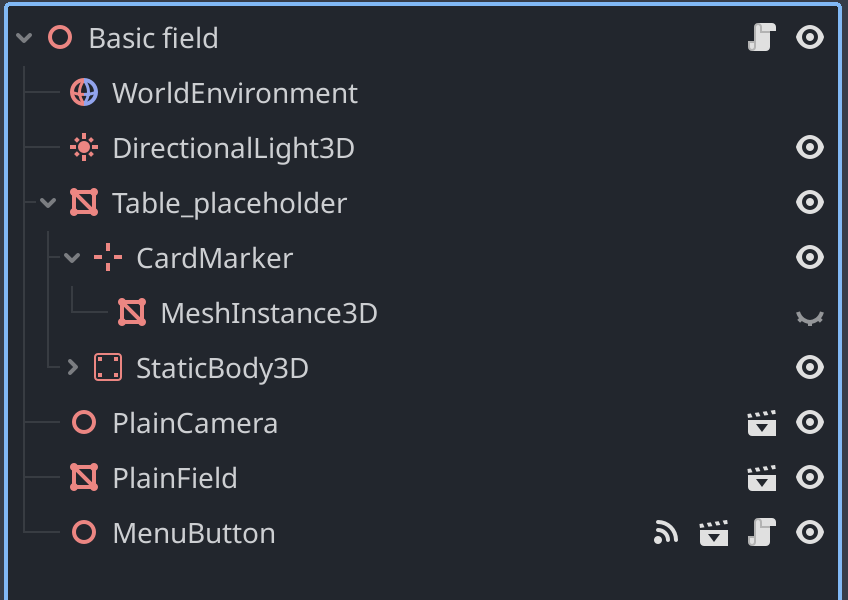
\includegraphics[width=0.5\textwidth]{img/basic_field_scene_structure.png}
    \caption{A játéktér Scene struktúrális felépítése}
    \label{img:basic_scene}  
\end{figure}
A scene kiszámolja, az előre beállított kártya szélesség, magasság és margó konstansok alapján, hogy a megkapott kártyák számát, a \lstinline|CardMarker| -höz képest hova kell lerakni (\ref{code:calculate_coordinate}. ábra)
\begin{figure}[H]
    \centering
    \begin{lstlisting}[language=GDScript]
        func _calculate_coordinate(i, j):
        return Vector3(
            TABLE.position.x + (((CARD_WIDTH  + MARGO) * CARD_SCALE) * i ) - (((CARD_WIDTH * CARD_ROW) - (CARD_WIDTH) + (MARGO*(CARD_ROW-1)))*CARD_SCALE / 2),
            TABLE.position.y,
            TABLE.position.z + (((CARD_HEIGHT  + MARGO) * CARD_SCALE) * j ) - (((CARD_HEIGHT * CARD_COLUMN) - (CARD_HEIGHT) + (MARGO*(CARD_COLUMN-1)))*CARD_SCALE / 2)
        )
    \end{lstlisting}
    \caption{Kártyák koordinátájának kiszámítása}
    \label{code:calculate_coordinate}
\end{figure}
Amint a \lstinline|Deck| objektum elküldi a \lstinline{cards_empty} signal-t, vagyis a játék végét, vagy ha a játékos megnyomja a Menü gombot, a játék visszatér a menübe. 

Más feladata nincs. 


\subsection{Deck}
A \lstinline|Deck| egy olyan globális objektum, mely a program futása során bármikor elérhető. A feladatai: 
\begin{enumerate}
\item Létrehozni a kártyákat, a játék kezdetekor (\ref{code:make_deck}. ábra)
\item Folyamatosan figyeli, hogy mely \lstinline|Card|-ok vannak még játékban a lstinline|cards| tömbben.
\item Kezeli a kártyák felfordítását. Ha két kártya azonos, akkor azokat kiveszi a listájából (\ref{code:talalat}. ábra).
\item Lementeni a játékos minden lépését a data tömbbe a memóriába. 
\item Figyeli a játék végét.
\item Lementeni a data tömböt egy JSON file-ba a játék végével.
\end{enumerate}

\begin{figure}[h]
    \centering
    \begin{lstlisting}[language=GDScript]
    func make_deck(card_pair_number: int, card_scene: PackedScene):
        data.card_pair_number = card_pair_number;
        cards.clear();
        for i in range(0, card_pair_number):
            var word = "";
            while ABC.find(word) > - 1 or word == "":
                word = generate_word('abcdefghijklmnopqrst', 1).to_upper();
            ABC.push_back(word);
            var card = card_scene.instantiate();
            #call_deferred("add_child", card);
            if card.has_method("set_label"):
                card.set_label(word);
            cards.push_back(card);
            cards.push_back(card.duplicate());
        cards.shuffle();
        data.card_labels = ABC;
    \end{lstlisting}
    \caption{Létrehozzuk a kártyákat}
    \label{code:make_deck}
\end{figure}
\begin{figure}[h]
    \centering
    \begin{lstlisting}[language=GDScript]
func talalat():
	if (chosenA.get_label() == chosenB.get_label()):
		cards.remove_at(cards.find(chosenA));
		cards.remove_at(cards.find(chosenB));
		chosenA.queue_free();
		chosenB.queue_free();
	else:
		chosenA.play_card_reflip_animation();
		chosenB.play_card_reflip_animation();
	chosenA = null;
	chosenB = null;
	can_flip = true;
	if cards.size() == 0 :
		cards_empty.emit()
		save_data()
    \end{lstlisting}
    \caption{Figyeljük a találatot}
    \label{code:talalat}
\end{figure}


\subsection{Card}
A kartyak vagyis Card scene (\ref{img:card_tree}. ábra) rendelkezik egy \lstinline|labellel| amelyet a \lstinline|Deck| add neki, a kártya létrehozásakor. Ez mondja meg, hogy milyen kártya. 
Egy játékmezőn pontosan két egyforma labellel rendelkező kártya szerepel(\ref{img:cards_has_pairs}. ábra).

\begin{figure}[H]
    \centering
    \begin{minipage}[b]{0.45\textwidth}
        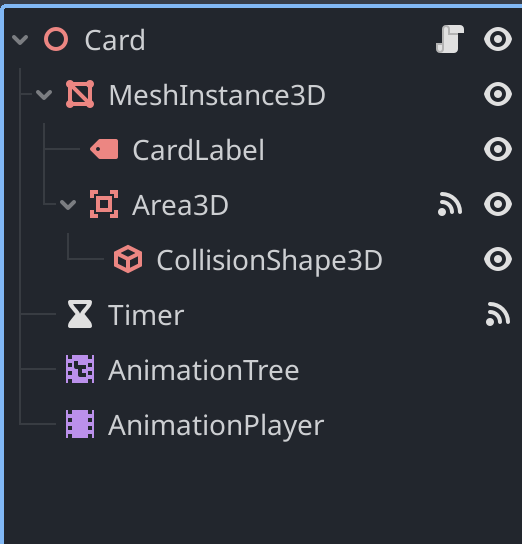
\includegraphics[width=\textwidth]{img/cards_scene_tree.png}
        \caption{A Card Scene struktúrája}
        \label{img:card_tree}
    \end{minipage}
    \hfill
    \begin{minipage}[b]{0.45\textwidth}
        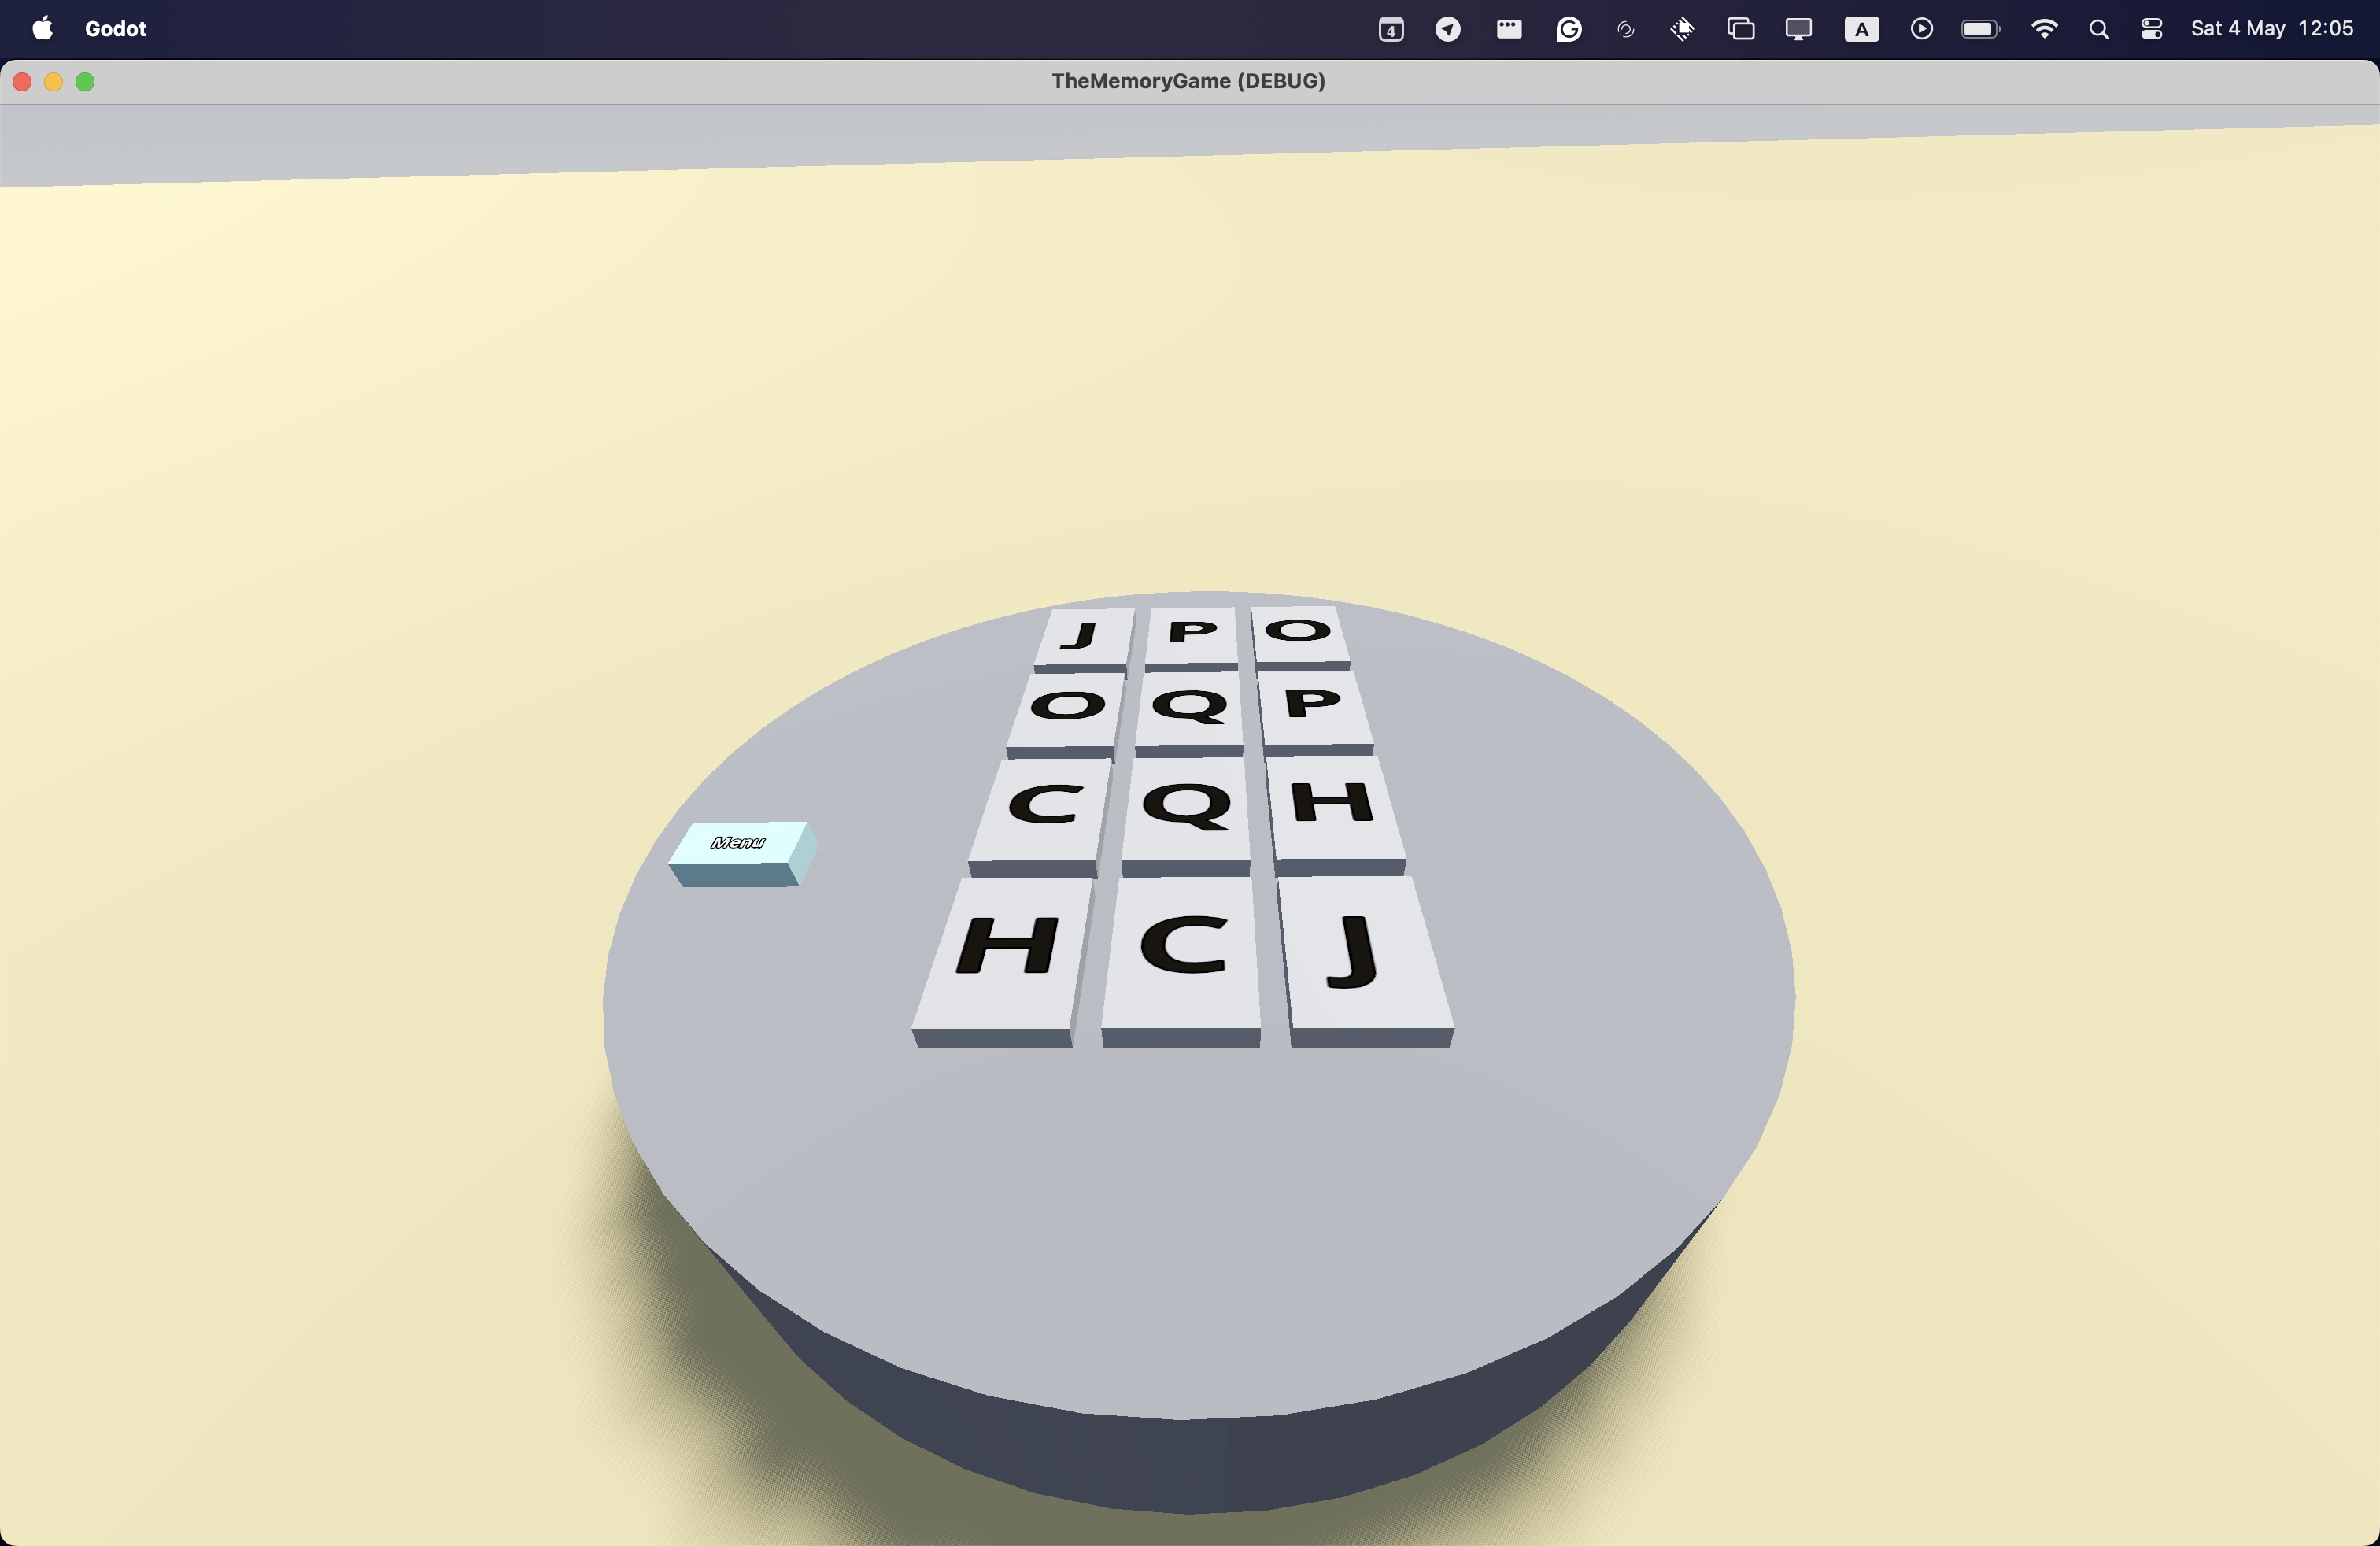
\includegraphics[width=\textwidth]{img/4x4_all_card_fliped.png}
        \caption{4x4 kártya. Minden betűből csak egy pár szerepel}
        \label{img:cards_has_pairs}  
    \end{minipage}
\end{figure}

A kártya rendelkezik animációval is, melyet az AnimationTree (\ref{img:animation_tree}. ábra) kezel. 
Ha rányomunk a kártyára, akkor lefut a \lstinline|card_flip_animation| function, vagyis az AnimationTree State Machine-nek odaadjuk azt az információt, mely szerint meg kell fordítani a kártyát. Az objektum elküldi önmagát a \lstinline|Deck|-nek, mint kiválasztott kártya. 
\begin{figure}[h]
    \centering
    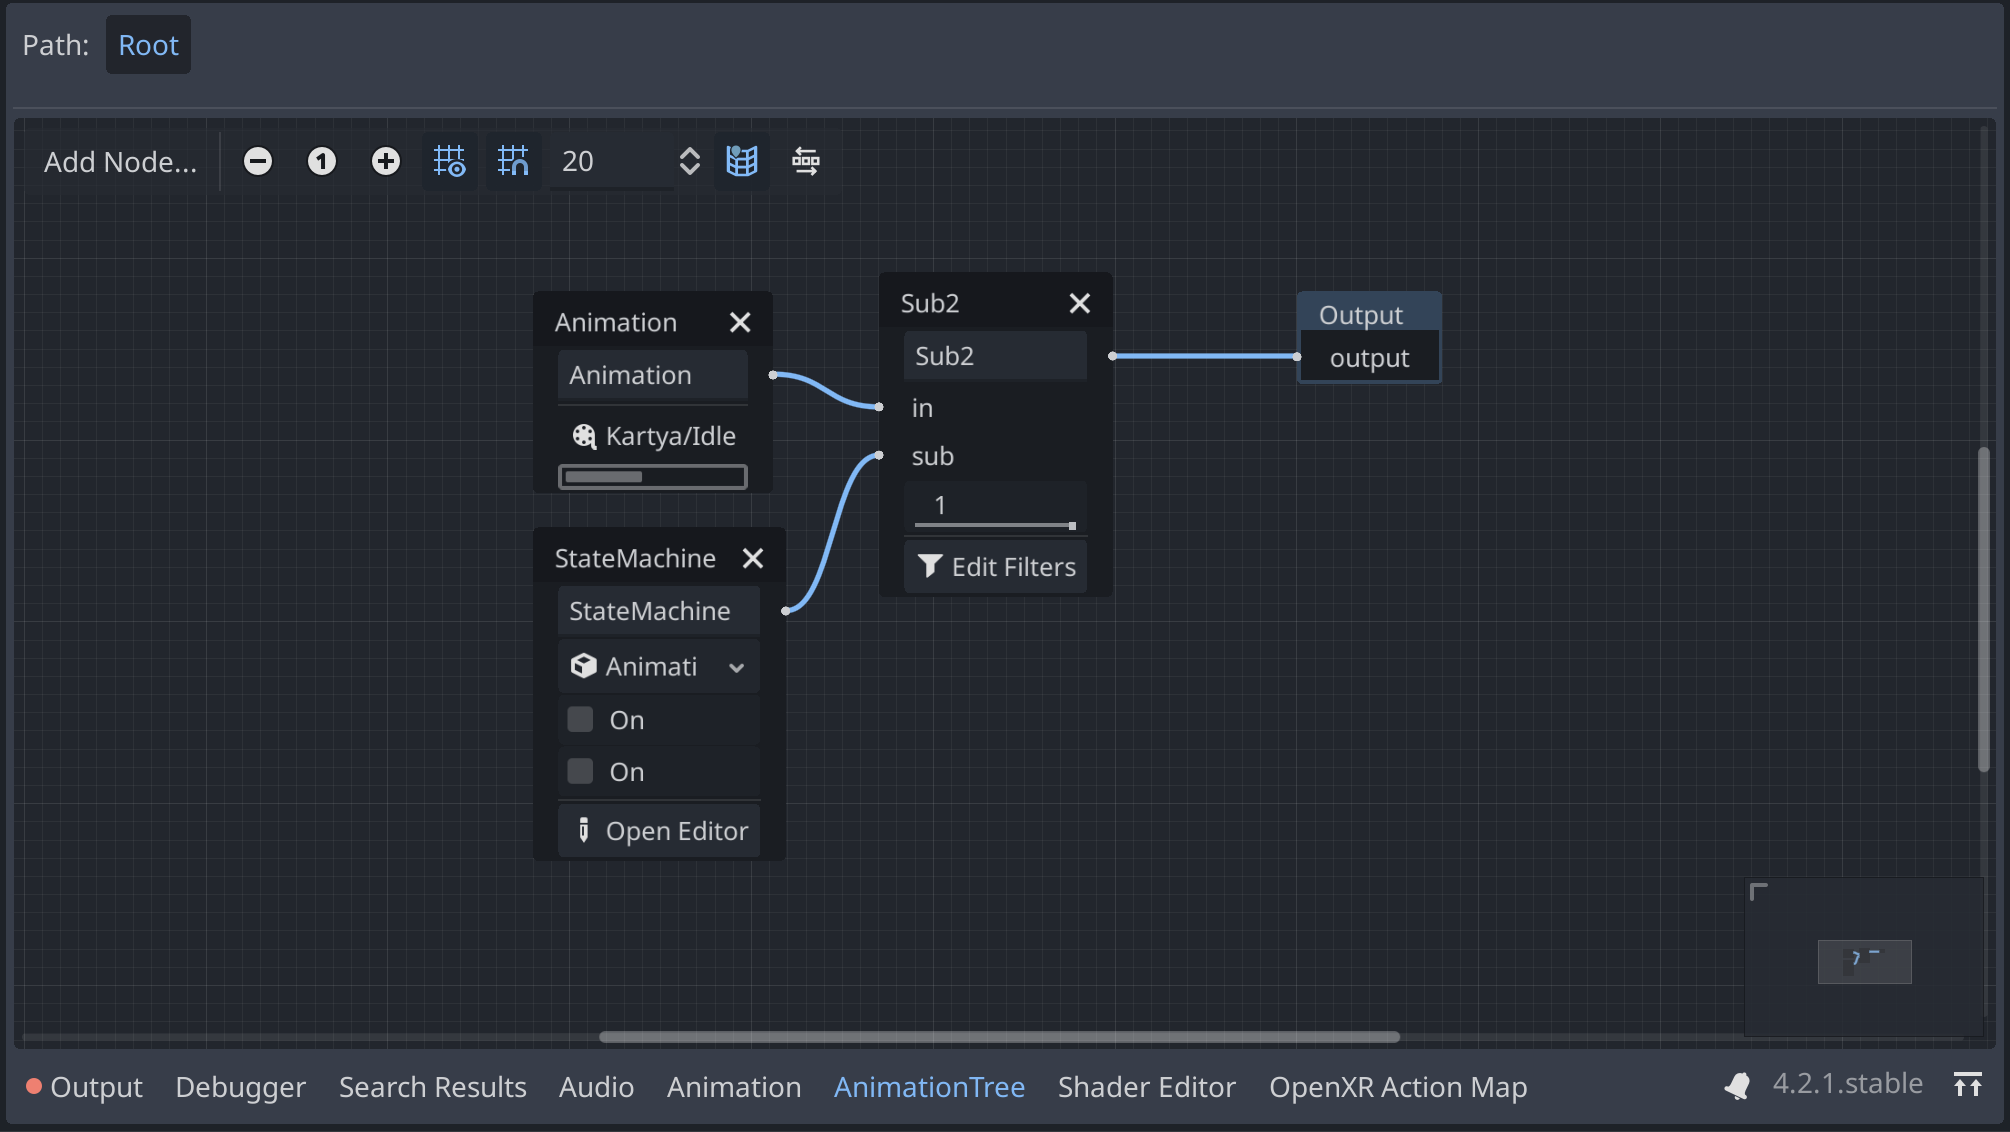
\includegraphics[width=\textwidth]{img/animation_tree.png}
    \caption{A Card animáció fája}
    \label{img:animation_tree}  
\end{figure}




	\chapter{Adatok gyűjtése a mesterséges intelligencia betanításához}
\thispagestyle{fancy}
\pagestyle{fancy}

\section{Tervezés}
A mesterséges intelligencia hatékony betanításához elengedhetetlen, hogy a lehető legtöbb információt gyűjtsük össze egy adott játékmenet során.

\subsection{Az adatszerkezet}
Egy adott játékfolyamat az alábbi lépésekből áll:

\begin{itemize}
\item A játékos a korábbi ismeretei alapján kiválasztja, melyik sor és melyik oszlop kártyáját fordítja fel.
\item A kártya felfordítása után a játékos megtudja, milyen betű található a kártyán.
\item Az így megszerzett információ és a korábbi tudása alapján a játékos kiválasztja a következő kártyát a táblán. Itt két lehetősége van:
\begin{itemize}
\item A játékos tudja, vagy nagy valószínűséggel sejti, melyik kártya a párja az előzőnek.
\item A játékos nem tudja, vagy kis valószínűséggel sejti, hol található a párja, ezért olyan kártyát fordít fel, amiről még nincs információja, azaz felfedezi a pályát.
\end{itemize}
\item Ha a felfordított kártyák párt alkotnak, azok eltűnnek a tábláról.
\item A játékos ezt a folyamatot addig ismétli, amíg az összes kártya el nem tűnik a tábláról.
\end{itemize}

A játék teljes megértéséhez és a mesterséges intelligencia betanításához az alábbi adatokra van szükségünk:

\begin{itemize}
\item A táblán található kártyák száma. Mivel mindig egy $N \cdot N$ négyzetet használunk, ezt az értéket fixen ismerjük.
\item A leosztásban szereplő betűk.
\item A kártyafordítások sorrendje: melyik sor és oszlop kártyái lettek felfordítva, valamint mi szerepelt a memória kártyán.
\end{itemize}

A következő adatszerkezetet használtam: 

\begin{figure}[h]
\centering
 \begin{lstlisting}
{
  "data": { 
    "id": "Xx12345"
    "played_games": {
      "6": [
        {
          "card_labels": ['A','B','C','D','E','F'], 
          "card_pair_number": 6,
          "card_selections": [ 
            {
              "chosen_first": true,
              "label": "A",
              "x": 0,
              "y": 0
            },
            {
                ...
            },
          ]
        },
        {
            ...
        }
      ]
    }
  }
}
\end{lstlisting}
\caption{Tanításhoz felhasznált adatszerkezet}
\label{saveJson}
\end{figure}


A \ref{saveJson} ábra magyarázata a következő:
\begin{description}
    \item[azonosító (id)] A játékos ID-je melyet megkap a játék elindításakor. 
    \item[Played\_games] Játszott játékok, ahol a kulcs a kártyapárok száma.
    \item[6\:] Egy tömb, amely az adott kártyaszámú játékokat tartalmazza.
    \item[card\_labels\:] A kártyák lehetséges címkéi. Ezek száma megegyezik a \lstinline{card_pair_number} értékével.
    \item[card\_pair\_number\:] A kártyapárok száma, amely megegyezik a tömb kulcsával. Az adatok könnyebb kezelése érdekében ez az érték duplikálva van.
    \item[card\_selections\:] Az összes kártyahúzás a játék során, ez a tömb a játék előrehaladtával bővül.
    \item[chosen\_first\:] Megjelöli, hogy a kártyát elsőként választották-e. Ez az információ a kártyaválasztások párosságából kiszámítható.
    \item[label\:] A kártyán szereplő betű.
    \item[X,Y\:] A kártya sor- és oszlopkoordinátái.
\end{description}
\subsection{Játék előkészítése}
A tervek szerint a játékot a lehető legtöbb emberhez akartam eljuttatni, ezért a legkézenfekvőbb megoldásnak a HTML5-be történő exportálást láttam \cite{Exportin97:online}. Ehhez néhány vizuális módosítást kellett végrehajtanom.
Két fő lehetőségem volt, amelyekkel komolyabban foglalkoztam:
\begin{enumerate}
    \item 	Játék és HTML sablon átalakítása: A játékot és a hozzá tartozó HTML sablont átírni úgy, hogy a weboldal JavaScriptje segítségével a JSON fájlt lementsem, amit aztán valamilyen online felületen keresztül el tudnak küldeni nekem.
\item	Fájl szerver létrehozása: Készítek egy fájl szervert, ahova a JSON-t minden sikeres játék után elküldöm egy HTTP kérés formájában.

\end{enumerate}


Átgondolva a lehetőségeimet, a fájl szerver mellett döntöttem, mivel így az összes tesztadat biztosan és automatikusan eljut hozzám.

A játékhoz készítettem egy \lstinline{http_client.gd} szkriptet, amelynek egyetlen feladata egy \lstinline{HTTP POST} kérés elküldése egy weboldalnak. A HTTP kérés törzsében helyeztem el a JSON fájlt. Ezt a szkriptet minden játék befejezése után aktiváltam.

Annak érdekében, hogy a kérés mindig sikeres legyen, biztosítanom kellett, 
hogy ha egy játékosnak nincs ID-je, akkor ha üresen hagyja a beviteli mezőt, 
és egy véletlenszerűen generált ID-t kapjon. 
Az ID-t a menü oldalon jelenítettem meg, és másolhatóvá tettem.
A játék állását, vagyis azt, hogy melyik játékkal mennyit játszott a játékos, a Godot automatikusan a böngésző lokális IndexedDB-jébe \cite{Exportin97:online} menti.
Az IndexedDB \cite{UsingInd44:online} egy böngésző alapú adatbázis, amely lehetővé teszi nagy mennyiségű strukturált adat tárolását, beleértve fájlokat és bináris adatokat is. Ez egy NoSQL adatbázis, ami azt jelenti, hogy kulcs-érték párokkal dolgozik, nem pedig táblázatokkal, mint egy relációs adatbázis. 
Az IndexedDB segítségével a memoriajáték elmentheti az adatait a böngészőbe, így később hozzáférhet és láthatja a játékos, hogy melyik nehézségi szinten mennyit játszott a játékkal.

Így, ha egy játékos akkor játszik, amikor a szerver nem elérhető, később is el tudja küldeni a játszott játékainak statisztikáját.\begin{figure}[h]
    \centering
    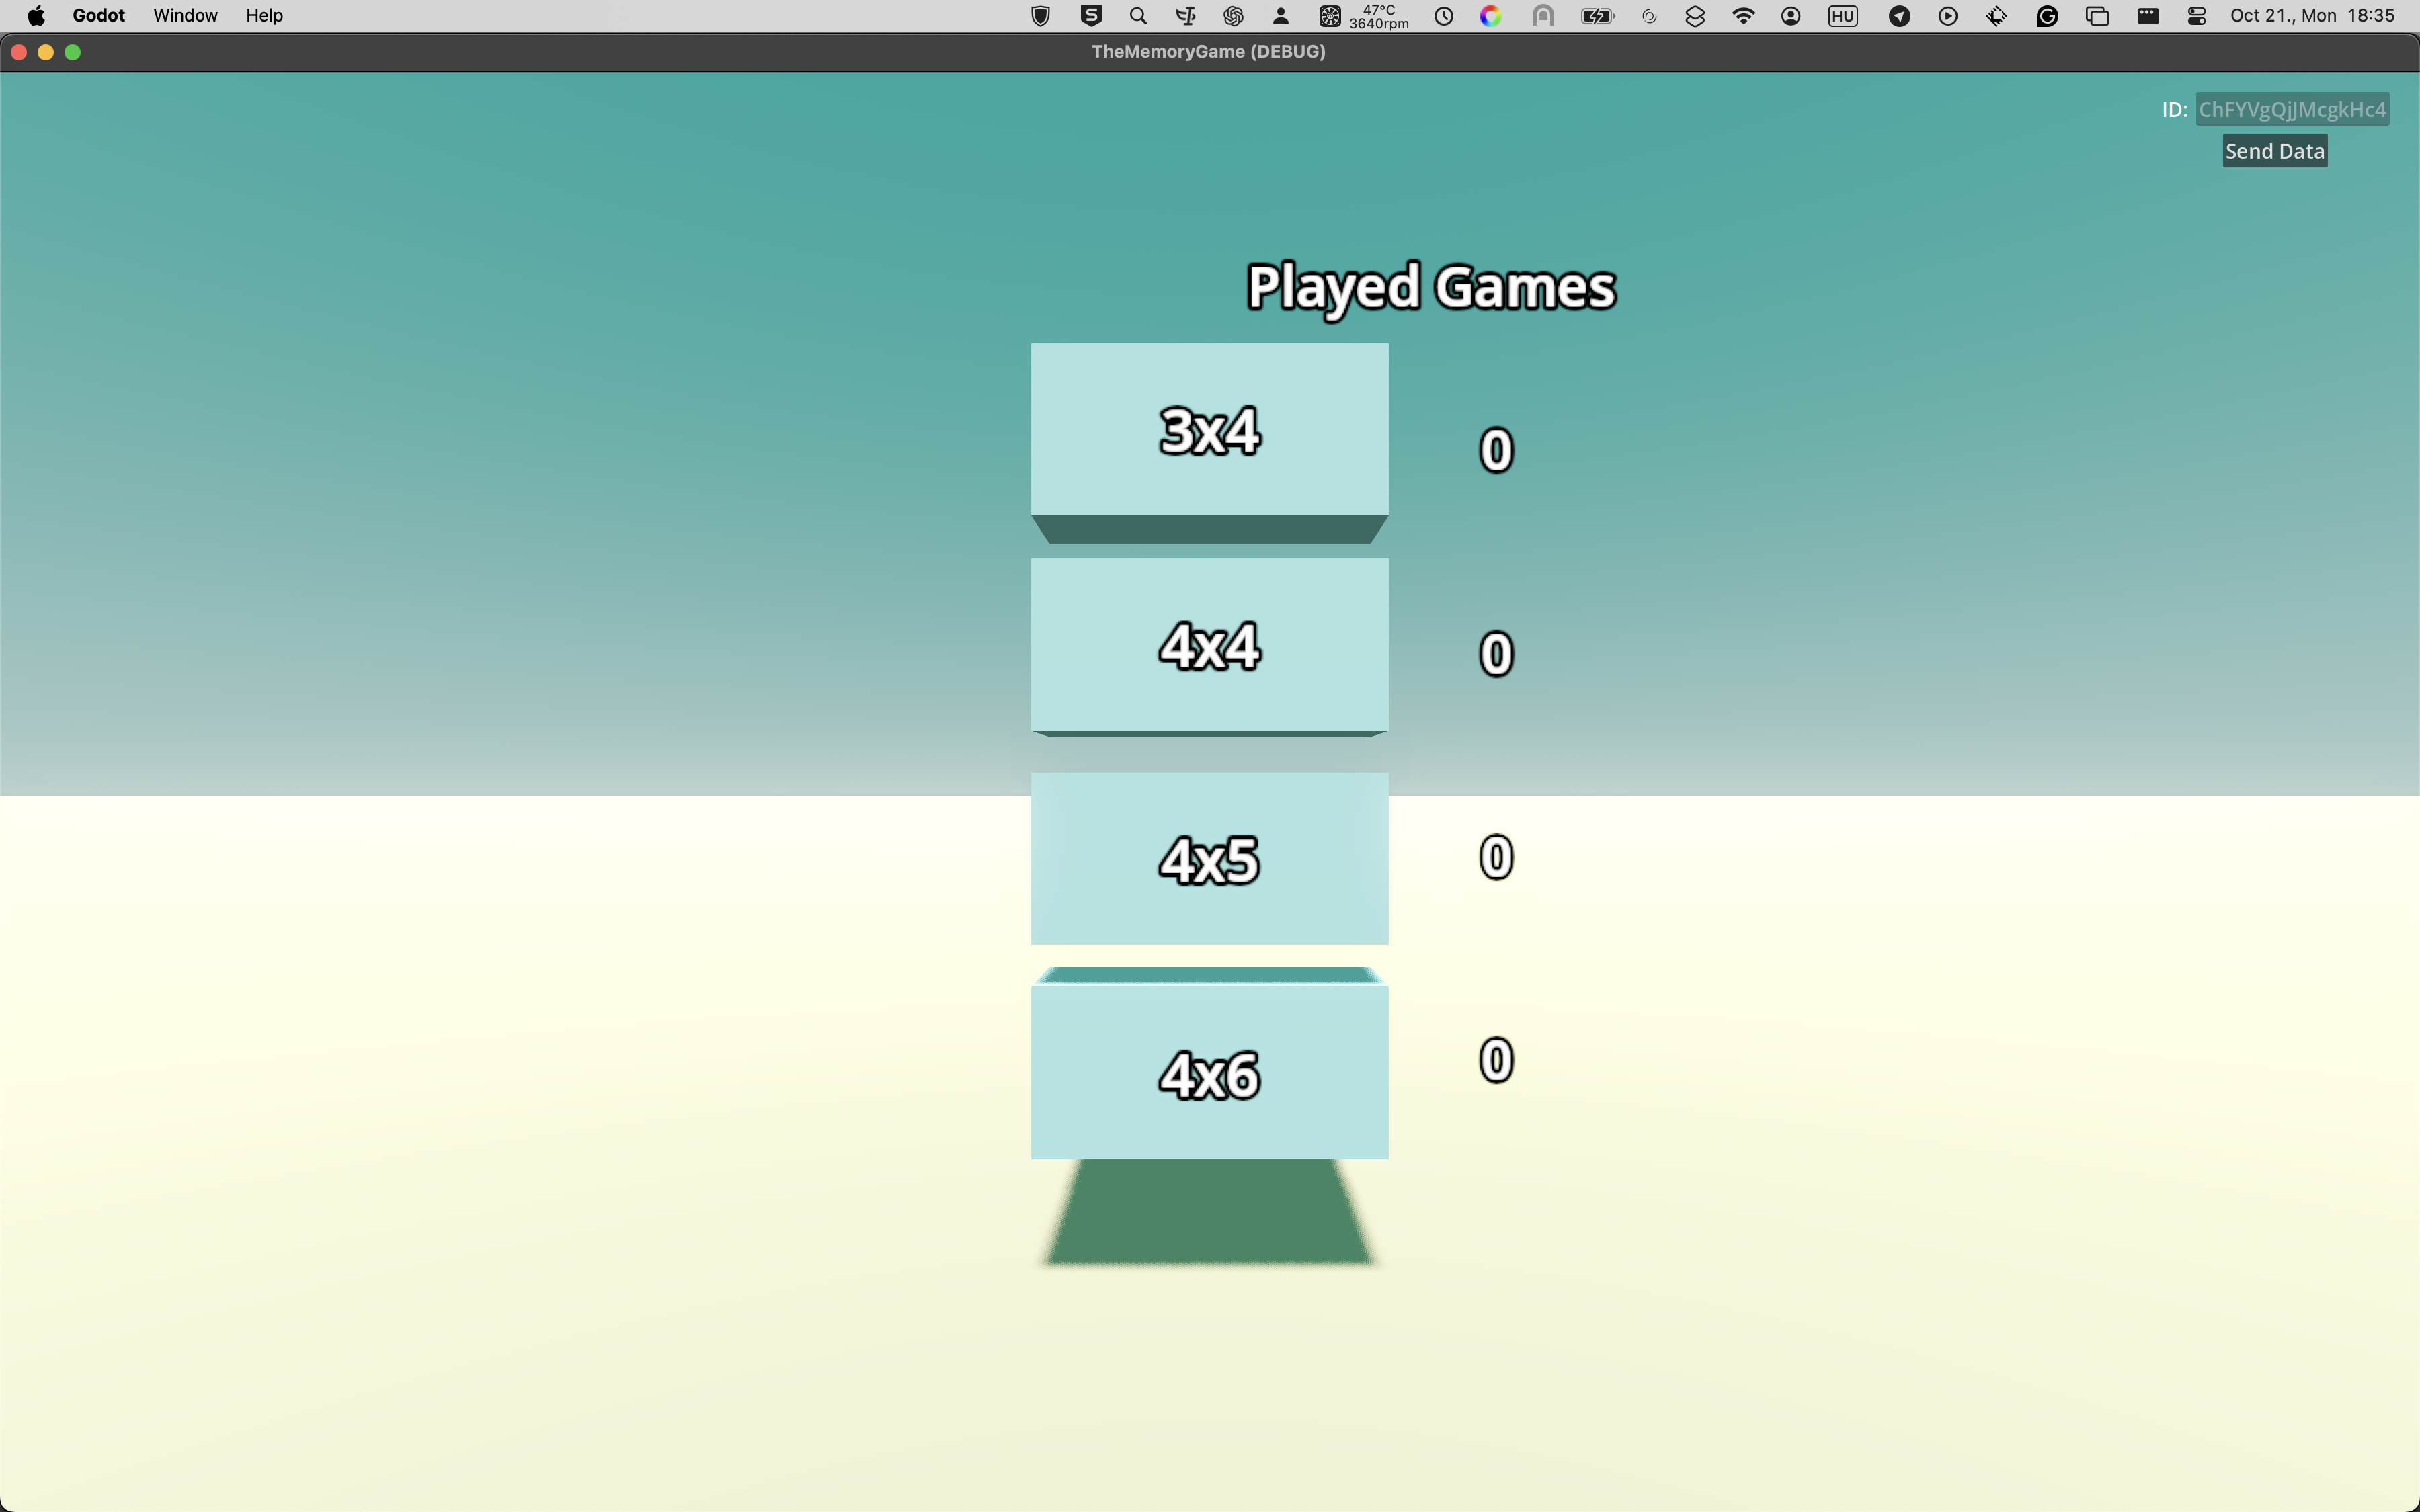
\includegraphics[width=0.75\textwidth]{img/menu_remake.png}
    \caption{Az átlakaított menü: másolható ID mező, és egy küldés gomb}
    \label{img:menu_remake}  
\end{figure}

\subsection{Játék feltöltése itch.io-ra}

A kész játékot exportáltam HTML5 formátumba, majd regisztráltam az itch.io oldalán.
Itt létrehoztam egy weboldalt a játékomnak, és elhelyeztem rajta egy rövidke leírást angolul.

A játékot elérhetővé tettem \url{https://csetom.itch.io/the-memory-game} címen (\ref{img:itch.io}. ábra). 

A beállítottam, hogy a "Run game" gombra kattintva a játék "teljes képernyős" üzemmódban induljon el, hogy kitöltse a teljes weboldalt. 

\begin{figure}[h]
  \centering
  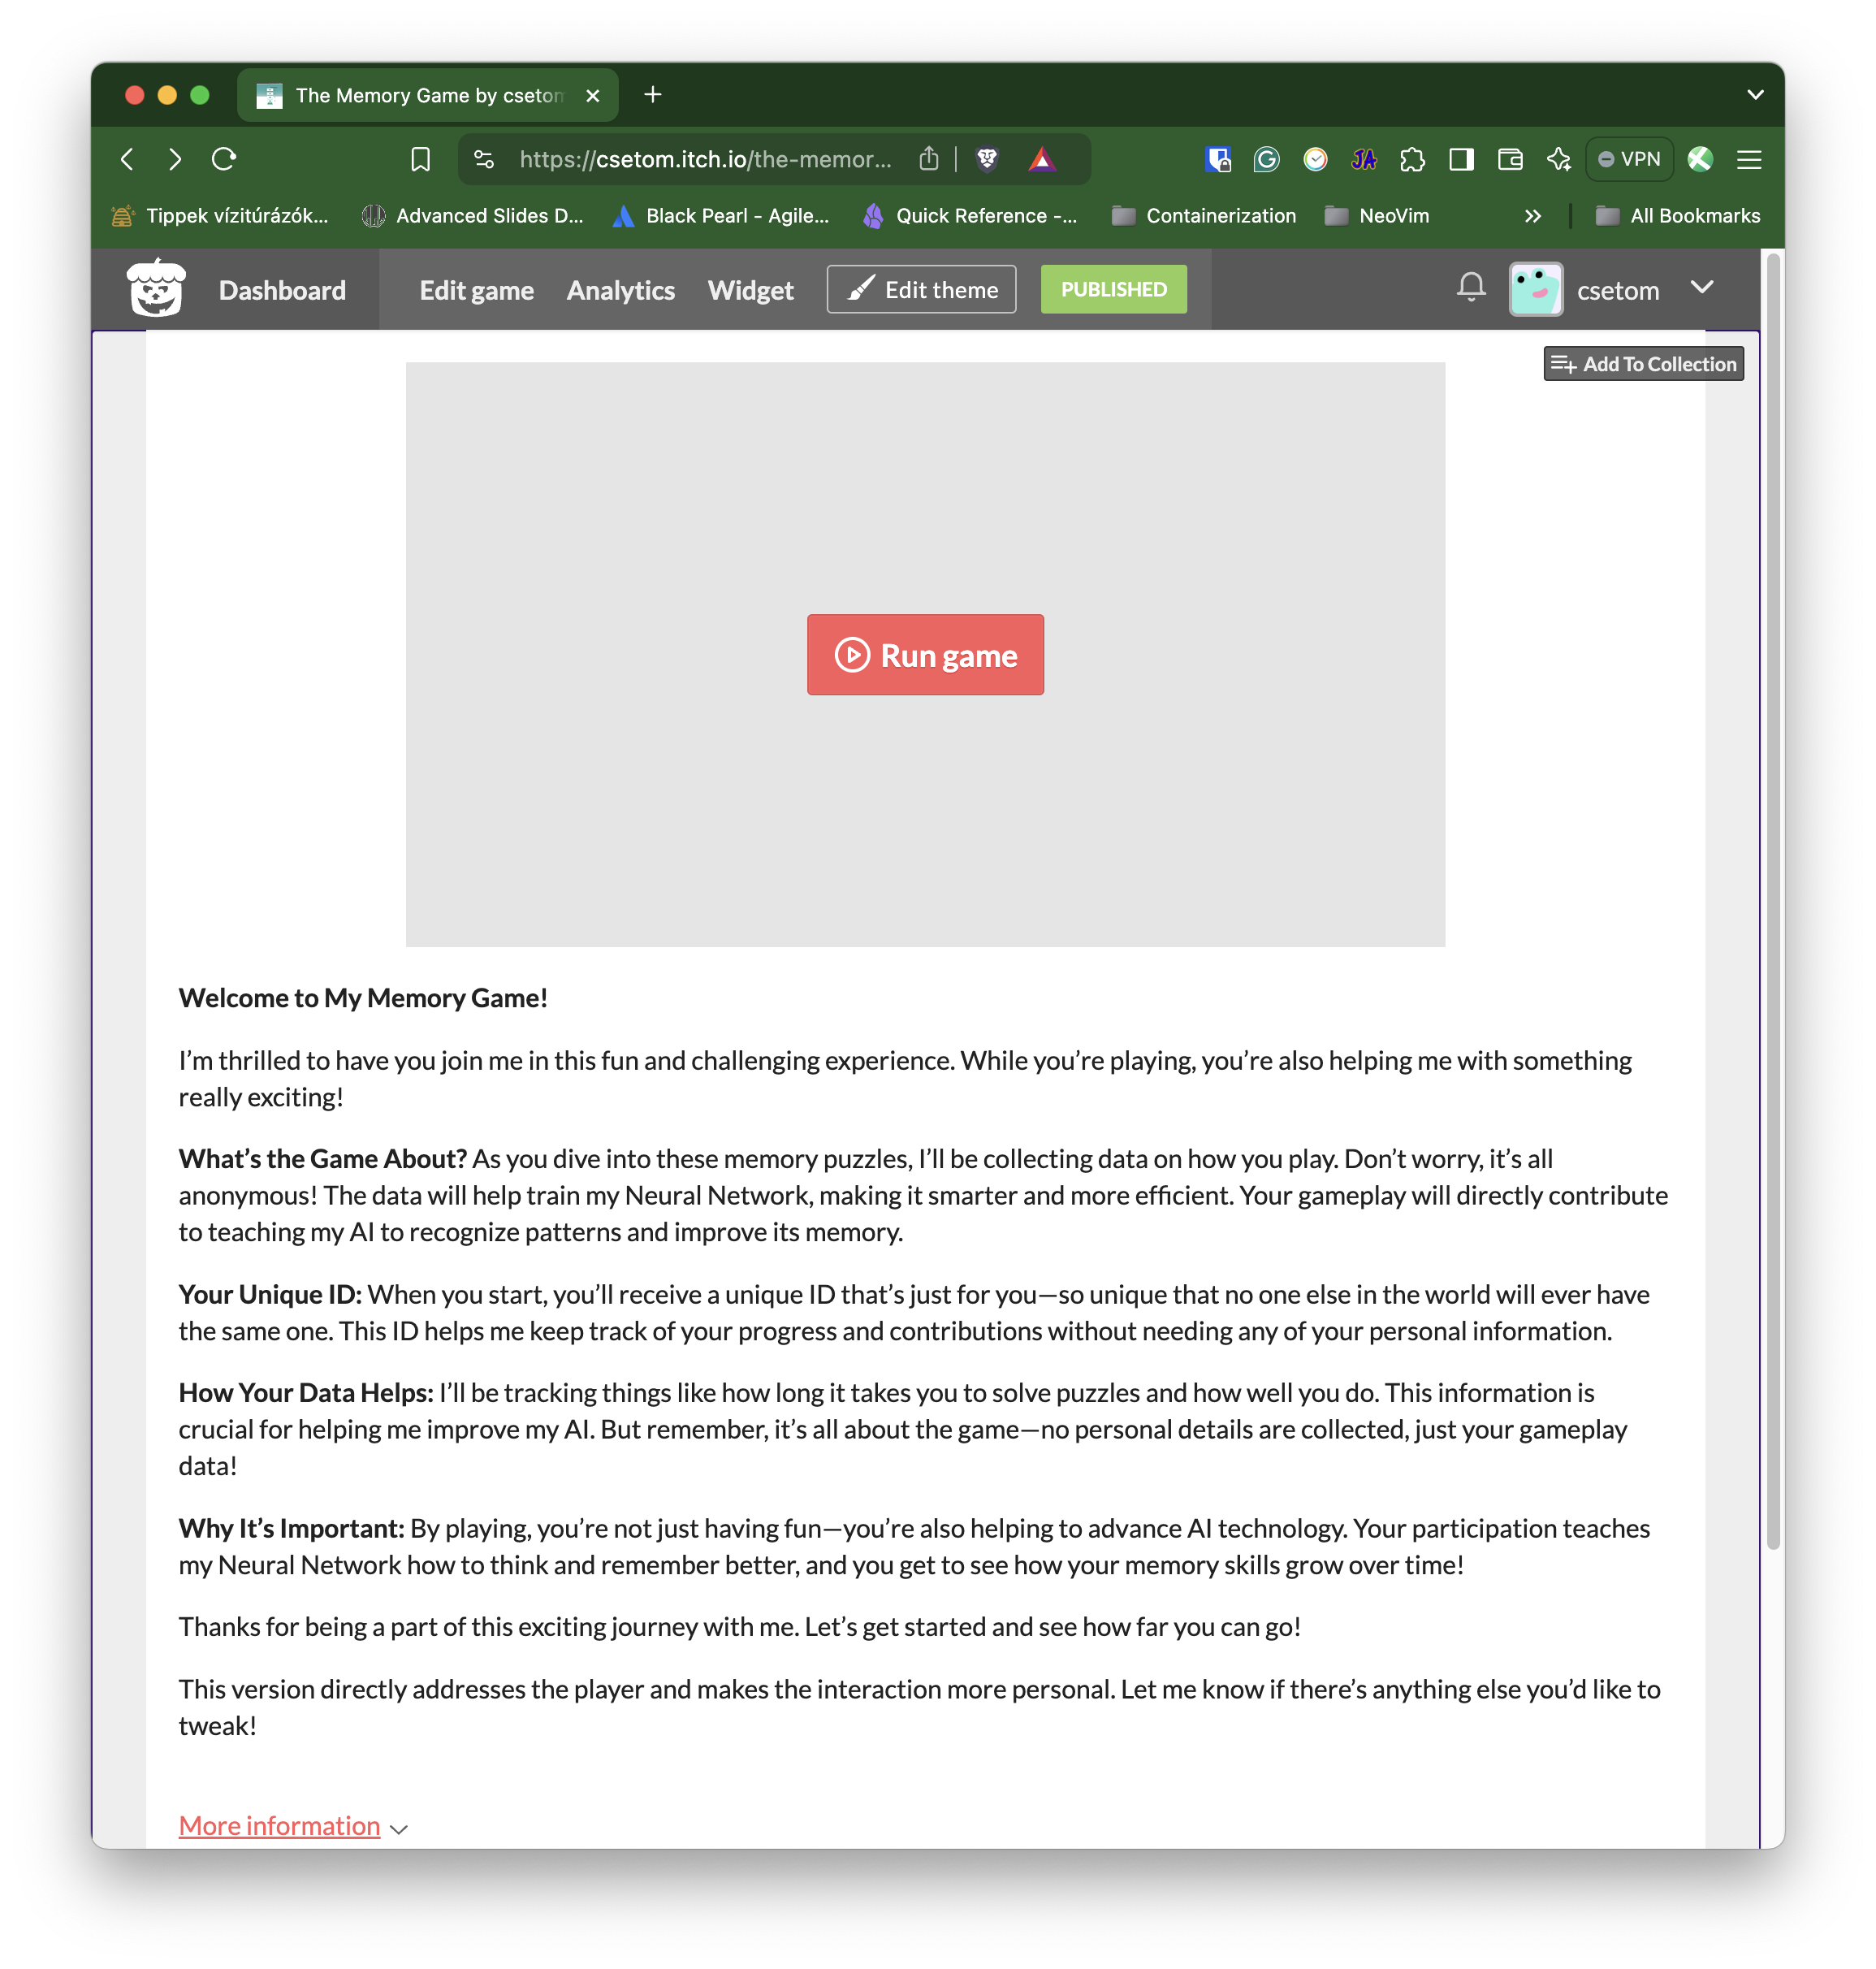
\includegraphics[width=0.75\textwidth]{img/Itch.io.png}
  \caption{Memóriajátékom itch.io oldala, ahonnan egy kattintásra futtatható a játék}
  \label{img:itch.io}  
\end{figure}


\section{Fájl szerver megvalósítása}
A fájlszerver megvalósításához JavaScriptet és Node.js-t használtam.
A szerver működtetésére az Express web framework-öt \cite{ExpressN40:online} vettem igénybe, 
A fájlszerver egyetlen végpontot biztosított, amely a \lstinline{/save_json} útvonalon volt elérhető. 
Ez a végpont fogadta az érkező JSON formátumú adatokat. A szerver feladata volt ezeknek az adatoknak a fájlrendszerbe történő mentése. 
A mentési folyamat során az adatok az ID szerint kerültek elhelyezésre külön mappákba, ahol a mappa neve a játékos ID-ja volt. 
Az egyes mappákban az aktuális időpont szerint elnevezett JSON fájlok kerültek tárolásra, például: \texttt{2023-10-21T12:34:56.json}. 
Ez a struktúra biztosította az adatok könnyű visszakereshetőségét és rendszerezhetőségét.

Annak érdekében, hogy a szerver domain néven keresztül is elérhető legyen, a Cloudflare Tunnel \cite{TunnelZe60:online} szolgáltatást alkalmaztam. 

A rendszer kényelmes használata és virtuális gépen történő telepítése érdekében a szervert és a Cloudflare-t is \cite{WhyCloud84:online} külön-külön Docker \cite{DockerAc99:online} konténerben futtattam.
A konténerek használata egyszerűvé teszi a telepítést és a menedzselést, mivel az alkalmazások és azok függőségei elszigetelten futnak. 
A Docker Compose \cite{DockerCo66:online} segítségével pedig könnyedén integrálhattam és menedzselhettem a többkonténeres alkalmazásokat, ami lehetővé tette a szerver és a Cloudflare Tunnel együttes futtatását és összehangolt működését.

\begin{figure}[h]
    \centering
\begin{lstlisting}
services:
file-server:
  build:
    context: .
  volumes:
    - ./data:/app/data
cloudflair:
  image: cloudflare/cloudflared:latest 
  command: tunnel --no-autoupdate run --token <token>
\end{lstlisting}
\caption*{docker-compose.yaml}
\label{code:docker-compose}
\end{figure}
\begin{figure}[h]
    \centering
    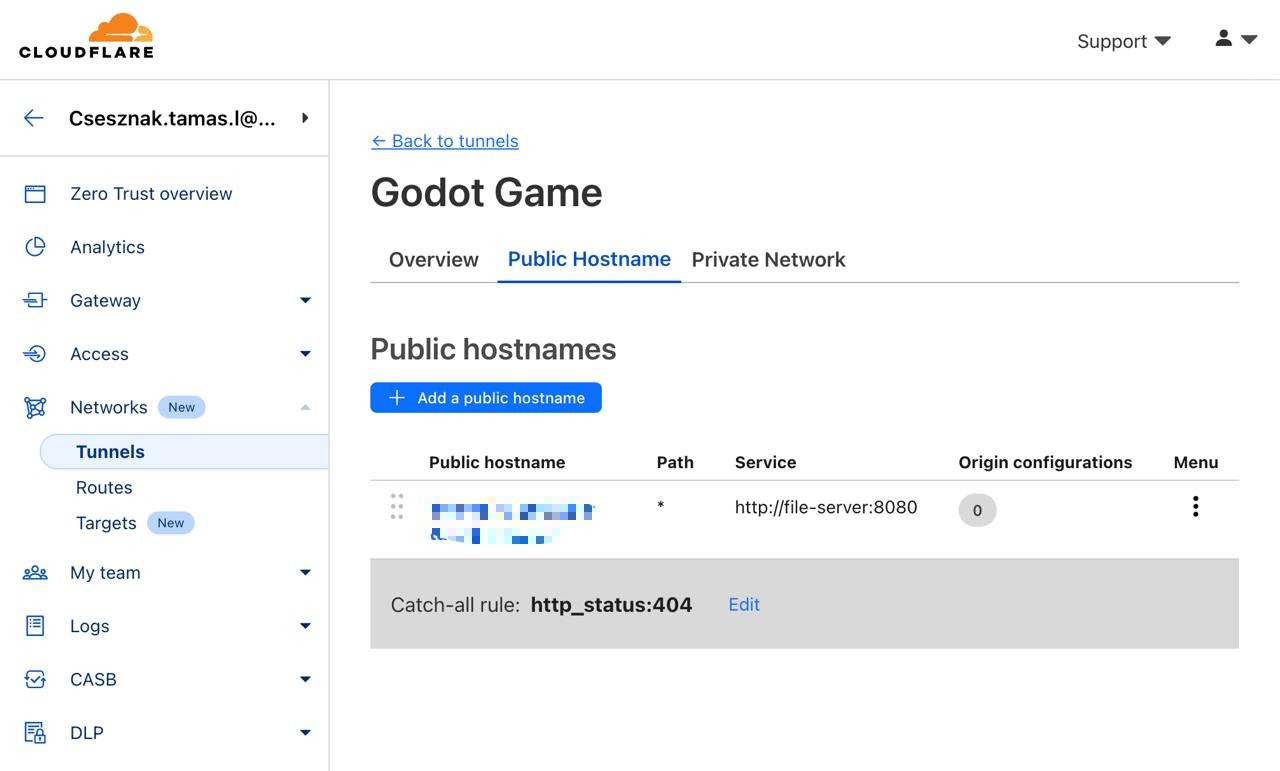
\includegraphics[width=0.75\textwidth]{img/cloudflair-censored.jpg}
    \caption{Cloudflair tunne konfiguráció}
    \label{img:cloudflair-config}  
\end{figure}


\subsection{Oracle Cloud}
A fájlszerver telepítéséhez először az Oracle VM-et \cite{CloudInf58:online} szerettem volna használni. Az Oracle VM egy rendkívül megbízható és skálázható megoldás, amely lehetővé teszi, hogy virtuális gépeket hozzunk létre és futtassunk különböző platformokon. Az Oracle VM számos előnnyel rendelkezik, mint például a magas teljesítmény, a robusztus biztonsági funkciók, és a kiváló támogatás. Ezen kívül számos operációs rendszerrel kompatibilis, ami megkönnyíti a különféle alkalmazások és szolgáltatások telepítését és futtatását.

Az Oracle VM-en keresztül kívántam a fájlszerveremet üzemeltetni, mivel reméltem, hogy a szolgáltatás rugalmassága és skálázhatósága előnyös lesz a projekt szempontjából. Az Oracle VM felületén könnyedén konfigurálhatók a virtuális gépek, és a hálózati beállítások is egyszerűen kezelhetők. Emellett a szolgáltatás integrálhatósága más Oracle termékekkel és szolgáltatásokkal további előnyöket kínál.

Azonban, amikor megpróbáltam igénybe venni az Oracle VM ingyenes erőforrásait, sajnálatos módon azt tapasztaltam, hogy ezek nem voltak elérhetők. Az ingyenes erőforrások hiánya miatt kénytelen voltam alternatív megoldást keresni, mivel nem tudtam megfelelően kihasználni az Oracle VM által nyújtott lehetőségeket. Ez komoly csalódást okozott, mivel úgy gondoltam, hogy az Oracle VM ideális lenne a fájlszerverem futtatására, de az ingyenes hozzáférés hiánya miatt további megoldásokat kellett keresnem.


\subsection{Fly.io}
Miután az Oracle VM nem bizonyult járható útnak, úgy döntöttem, hogy kipróbálom a Fly.io \cite{Deployap0:online} szolgáltatását.
A Fly.io egy modern felhőalapú platform, amely lehetővé teszi az alkalmazások globális szinten történő futtatását és skálázását. A szolgáltatás fő célja, hogy az alkalmazásokat közelebb hozza a felhasználókhoz, ezáltal csökkentve a késleltetést és javítva a teljesítményt. A Fly.io platformja rendkívül egyszerűen használható, és számos automatizált funkcióval rendelkezik, amelyek megkönnyítik az alkalmazások telepítését és kezelését.

A Fly.io honlapja első ránézésre ígéretesnek tűnt, és úgy tűnt, hogy ingyenes használati lehetőséget is kínál. Ez különösen vonzó volt számomra, mivel szerettem volna minimalizálni a költségeket a projekt korai szakaszában. A Fly.io segítségével könnyedén létrehozhattam és kezelhettem a fájlszerveremet, és a platform egyszerűsége miatt gyorsan és hatékonyan tudtam dolgozni.

Azonban, amikor elkezdtem a fájlszerver telepítését és konfigurálását a Fly.io platformján, kiderült, hogy a szolgáltatás nem teljesen ingyenes.
A Fly.io használatával kapcsolatos üzenetváltások darabszámára vonatkozó díjak jelentősen 
megnövelték volna a költségeket. Ez komoly kihívást jelentett, és nem számítottam ilyen jellegű kiadásokra. 
Az ingyenesnek tűnő szolgáltatásról kiderült, 
hogy valójában nem az. Csalódtam, és ismét arra kényszerűltem, hogy más megoldásokat keressek a fájlszerverem üzemeltetéséhez.

Mindkét esetben a szolgáltatások ígéretes lehetőségeket kínáltak, de végül nem feleltek meg az elvárásaimnak az ingyenes erőforrások hiánya és a rejtett költségek miatt. Azonban a tapasztalatok segítettek abban, hogy jobban megértsem a különböző felhőalapú platformok működését és költségstruktúráját, ami hasznos lesz a jövőbeni projektek tervezésénél és megvalósításánál.
\section{Végleges megoldás}
Mivel sajnos nem találtam más alternatívát, ami ingyenes lenne, így kénytelen voltam a helyi gépemen futtatni a docker containereket, és megkérni a játék tesztelőket, hogy akkor futtassák a játékot, amikor éppen üzemel a file szerver. A tesztelőknek elküldtem az itch.io weboldalt, így nem volt szükséges számukra, hogy telepítsék a saját számítógépükre az alkamazást.

Összesen tíz embertől sikerült megfelelő mennyiségű adatot szereznem,melynek segítségével tanítottam be a mesterséges intelligenciát.

	\chapter{Mesterséges intelligencia betanítása és használata}
\thispagestyle{fancy}
\pagestyle{fancy}


A célom az volt, hogy a mesterséges intelligencia játéka, a lehető legjobban hasonlítson az emberi gondolkodáshoz. Az emberi agy működéséhez a legjobban 
a neurális hálózat hasonlítható, így ezt használtam én is a projektemhez. 



\section{TensorFlow}
Python nyelven terveztem elkészíteni az MI tanításához az algoritmust. Ehhez a legjobbnak a TensorFlow-t \cite{tensorflow2015-whitepaper} találtam.
A TensorFlow weboldalán ingyenesen elérhető dokumentációkból és tanító anyagokból indultam ki. 

A dokumentáció szerint, minden felhasználónak alapvetően a Keras API \cite{chollet2015keras} használatát javasolják, így hát én is azt használtam. 

\section{Tervezés}
Az elképzelésem szerint, egy Sequential, azaz szekvenciális modellt használtam. A szekvenciális modellben pontosan egyetlen egy bemeneti tensor és egyetlen egy kimeneti tensor található.

Az én esetemben a bemeneti tensor a játék jelenlegi állása volt, a kimenet pedig a következő felfordítandó kártya lett. Mivel a tensornak a típusa nem változott, pusztán az értéke, ezért nekem ez tökéletesen megfelelő volt.

A modellt be kellett tanítanom a gyűjtött adatokkal. Ehhez a legegyszerűbb az volt, ha az adataimat egy JSON fájlba összefűztem, így a scriptnek elég volt ezt az egy fájlt beolvasnia.

Minél jobban le tudtam egyszerűsíteni a bemeneti rétegem, úgy, hogy lehetőleg ne legyen benne adatvesztés, annál gyorsabban véghez tudtam vinni a tanítást. 
Ha bonyolult volt az input layer, akkor a tanulás lelassult, és számomra fontos perceket, órákat, de akár napokat is veszíthettem volna egy hibás modell esetén.

Példának okáért, tegyük fel, hogy nem transzformálom át a gyűjtött adatokat, és a játék $N$ lépésből áll. 
Mivel mind az $N$ esetben az előző $N-1$ lépést is oda kell adnom a tanító algoritmusnak, és 1.-től $N.$-ik lépésig az összes lépést meg kell tanítanom a modellnek, 
így egy $N$ lépésből álló játéknak a tanításhoz felhasznált adatmennyisége:

\begin{equation}\label{eq:1}
\frac{N(N+1)}{2} = \frac{N^2+N}{2}
\end{equation}

Látható, hogy négyzetesen nő az adatok mennyisége. Annak érdekében, hogy ezt elkerüljem, a következő ötlettel álltam elő:

A hash-függvényeket az informatikában az 1980-as évek óta alkalmazzák arra, hogy bármilyen méretű adatot rögzített hosszúságúra alakítsanak át. Gyakorlati felhasználási területük például a fájlok ellenőrzése. 
Ha két fájl tartalma teljesen megegyezik, akkor az azokból képzett hash is azonos lesz. 
Ez különösen hasznos, amikor dokumentumokat töltünk fel egy fájlszerverre, így könnyen ellenőrizhető, hogy a fájl már létezett-e a szerveren, és elkerülhető a duplikált tárolás.

A hash-függvények segítségével képes voltam minden lépést és az őt megelőző összes eddigi lépés együttesét fix hosszú bit vektorrá átalakítani, így szignifikáns mennyiségű adatmennyiséget tudtam spórolni.
Természetesen fennállt annak a lehetősége, hogy a betanított modellem nem lesz teljesen pontos, azonban ez a kockázat minden transzformációs folyamat során előfordulhat.

\begin{figure}[h]
    \centering
    \begin{adjustbox}{width=0.75\textwidth}
        \label{diagram:deepLearningModel}  
        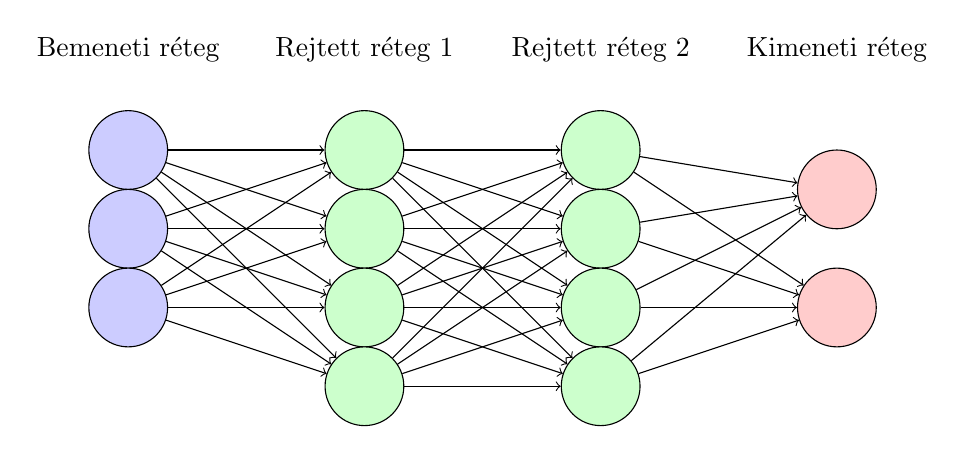
\begin{tikzpicture}[
            node distance=1.5cm and 2cm,
            input neuron/.style={circle, draw, fill=blue!20, minimum size=1cm},
            hidden neuron/.style={circle, draw, fill=green!20, minimum size=1cm},
            output neuron/.style={circle, draw, fill=red!20, minimum size=1cm},
            neuron missing/.style={draw=none, fill=none, text height=0.5cm, execute at begin node=\color{black}$\vdots$}
        ]
        
        % Input layer
        \foreach \m in {1,2,3}
            \node[input neuron] (I-\m) at (0,-\m) {};
        
        % Hidden layer 1
        \foreach \m in {1,2,3,4}
            \node[hidden neuron] (H1-\m) at (3,-\m) {};
        
        % Hidden layer 2
        \foreach \m in {1,2,3,4}
            \node[hidden neuron] (H2-\m) at (6,-\m) {};
        
        % Output layer
        \foreach \m in {1,2}
            \node[output neuron] (O-\m) at (9,-1.5*\m) {};
        
        % Connect input layer to hidden layer 1
        \foreach \i in {1,2,3}
            \foreach \j in {1,2,3,4}
                \draw[->] (I-\i) -- (H1-\j);
        
        % Connect hidden layer 1 to hidden layer 2
        \foreach \i in {1,2,3,4}
            \foreach \j in {1,2,3,4}
                \draw[->] (H1-\i) -- (H2-\j);
        
        % Connect hidden layer 2 to output layer
        \foreach \i in {1,2,3,4}
            \foreach \j in {1,2}
                \draw[->] (H2-\i) -- (O-\j);
        
        % Labels
        \node[above] at (0,0) {Bemeneti réteg};
        \node[above] at (3,0) {Rejtett réteg 1};
        \node[above] at (6,0) {Rejtett réteg 2};
        \node[above] at (9,0) {Kimeneti réteg};
        
        \end{tikzpicture}
    \end{adjustbox}
    \caption{Neurális háló, egy bemeneti, két rejtett és egy kimeneti réteggel}
\end{figure}

\section{Adatok transzformálása}

Az adatok transzformálását a program futása közben, felhasználás előtt készítettem elő. Ez azért volt hasznos, mivel a játék közben, a kész modell felhasználásakor is dinamikusan kellett az adatokat hash-függvénnyel leképeznem.

\begin{itemize}
    \item Beolvasom a JSON állományt. 
    \item Végigmegyek az adatokon, és létrehozok egy szöveges változót. Ez a változó tartalmazza a JSON-ban található aktuális valamint az összes előző lépést  (\ref{code:json_to_hash}. ábra). 
    \item A python hashlib csomagja segítségével ezt a változót leképezem az SHA256 függvényt használva egy hexadecimális stringgé. 
    \item A leképezett hexadecimális stringet tovább transzformálom. 
    Végigmegyek az összes karakterén, minden karakter egy hexadecimális szám. Ezen számokat leképezem egy decimális számmá, majd tovább konvertálom egy 4 bit hosszú binárissá. Ezen 4 számjegyű számokat összefűzöm egy stringgé, majd átkonvertálom, hogy egy darab 256 bitből álló NumPy tömböt kapjak, melyet fel fogok tudni használni a tanításhoz (\ref{code:hash_to_bit}. ábra). 
\end{itemize}

\begin{figure}[h]
    \center
    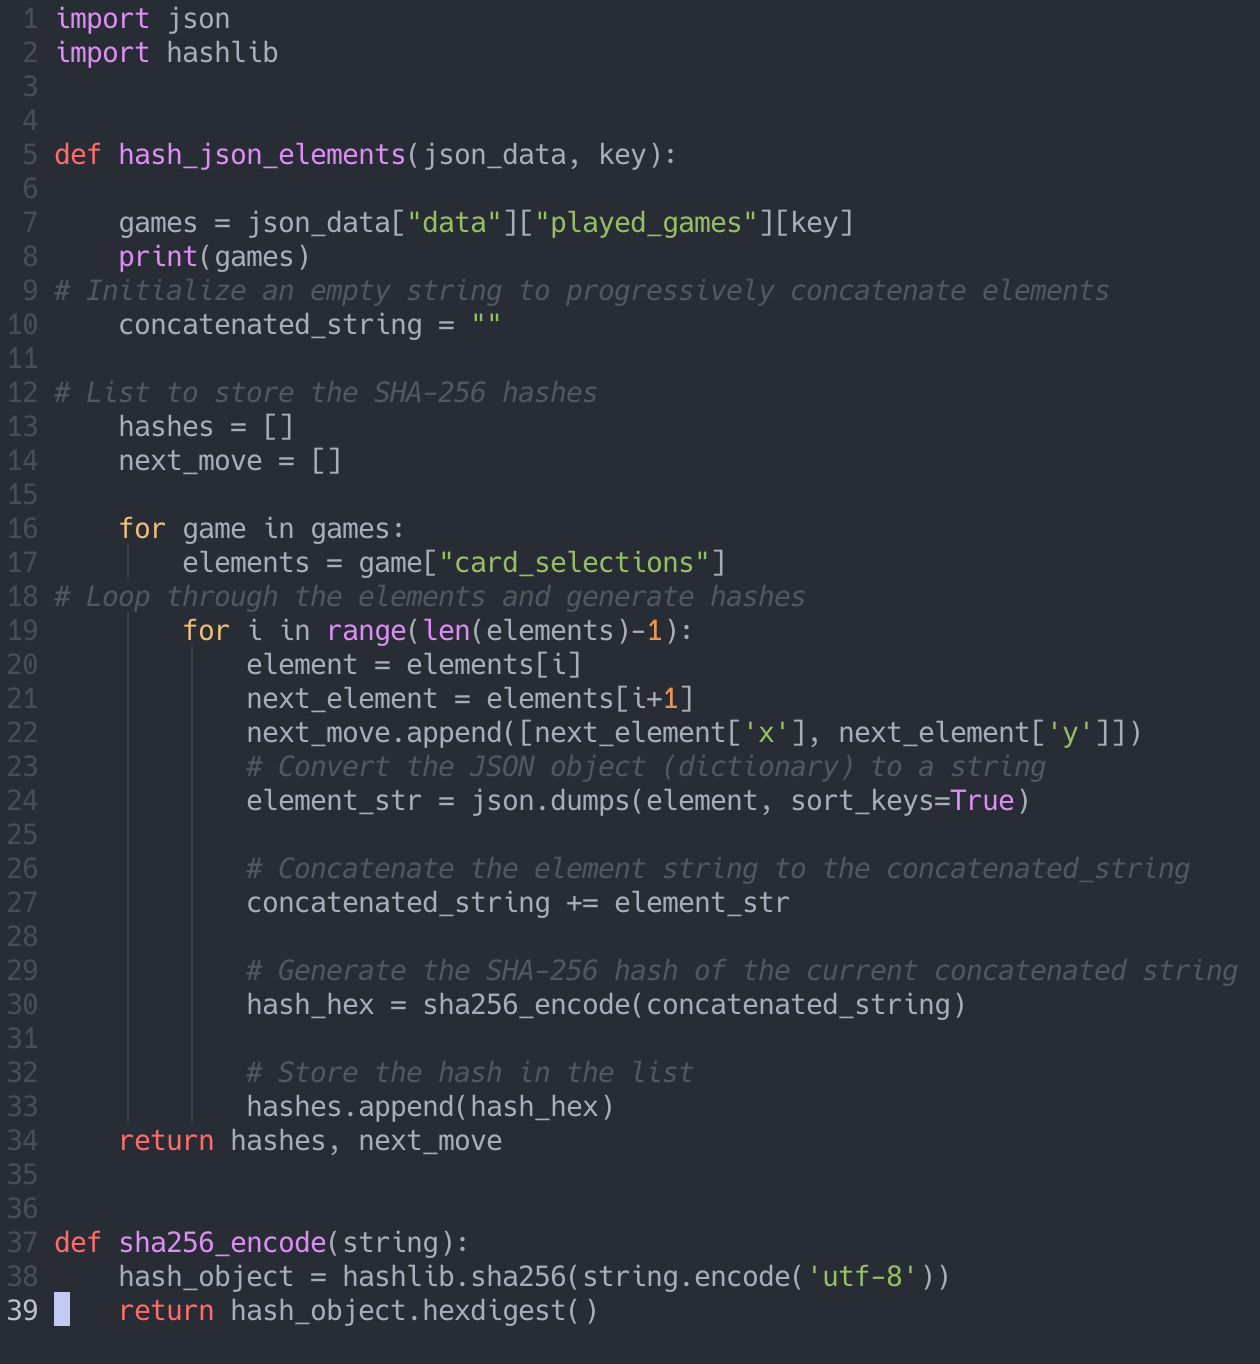
\includegraphics[width=0.50\textwidth]{img/JSON_TO_SHA256.png}
    \caption{Kód részlet, amely leképezi a \lstinline{key} által megadott játék lépéseit egy hash tömbbé. A hash-ek mellett a következő lépéseket tartalmazó tömbbel tér vissza.}
    \label{code:json_to_hash}
\end{figure}

\begin{figure}[h]
    \center
    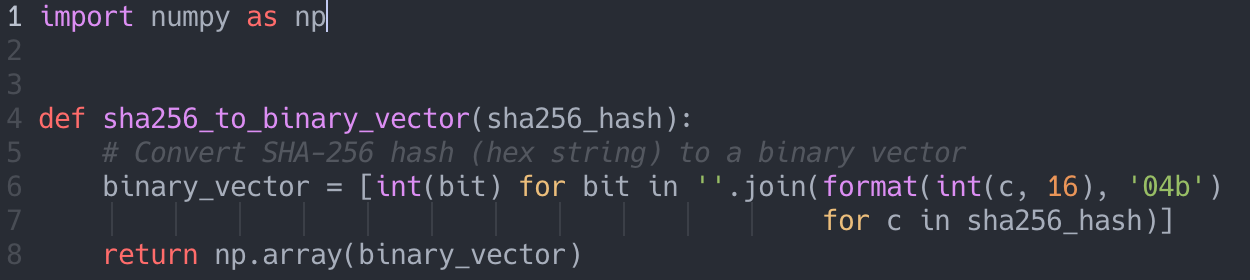
\includegraphics[width=0.50\textwidth]{img/hash_to_bit.png}
    \caption{Kód részlet. Az SHA256 hash hexadecimális string bitsorozattá konvertálása.}
    \label{code:hash_to_bit}
\end{figure}

\section{A tanító algoritmus}

\subsection{A modell elkészítése}
A TensorFlow része a Keras API, mely segítségével könnyedén és egyszerűen létre tudok hozni szekvenciális modellt (\ref{code:tensor}. ábra). A modell bemeneti rétege egy 256 nagyságú tömböt vár, melyben bitek találhatók. 

A következő két réteghez egy 128 és egy 64 neuront tartalmazó teljesen kapcsolodó (Dense) réteget használok. Dense layer azt jelenti, hogy a réteg összes neuronja kapcsolodik az előző réteg összes neuronjával. Ez a neuron típus gyarkan használt előre csatolt neurális hálóknál.
Az aktivációs függvény, amit ezekhez a rétegekhez használok, az az úgynevezett 
ReLU (Rectified Linear Unit) függvény, mely a következőképpen néz ki:
\begin{equation}\label{eq:2}
\text{ReLU}(x) = \max(0, x) 
\end{equation}

ami azt jelenti, hogy ha bemeneti érték, vagyis $x$ pozitív, akkor $x$-et adja vissza, ha negatív, akkor 0-t. 


\begin{figure}[h]
    \center
    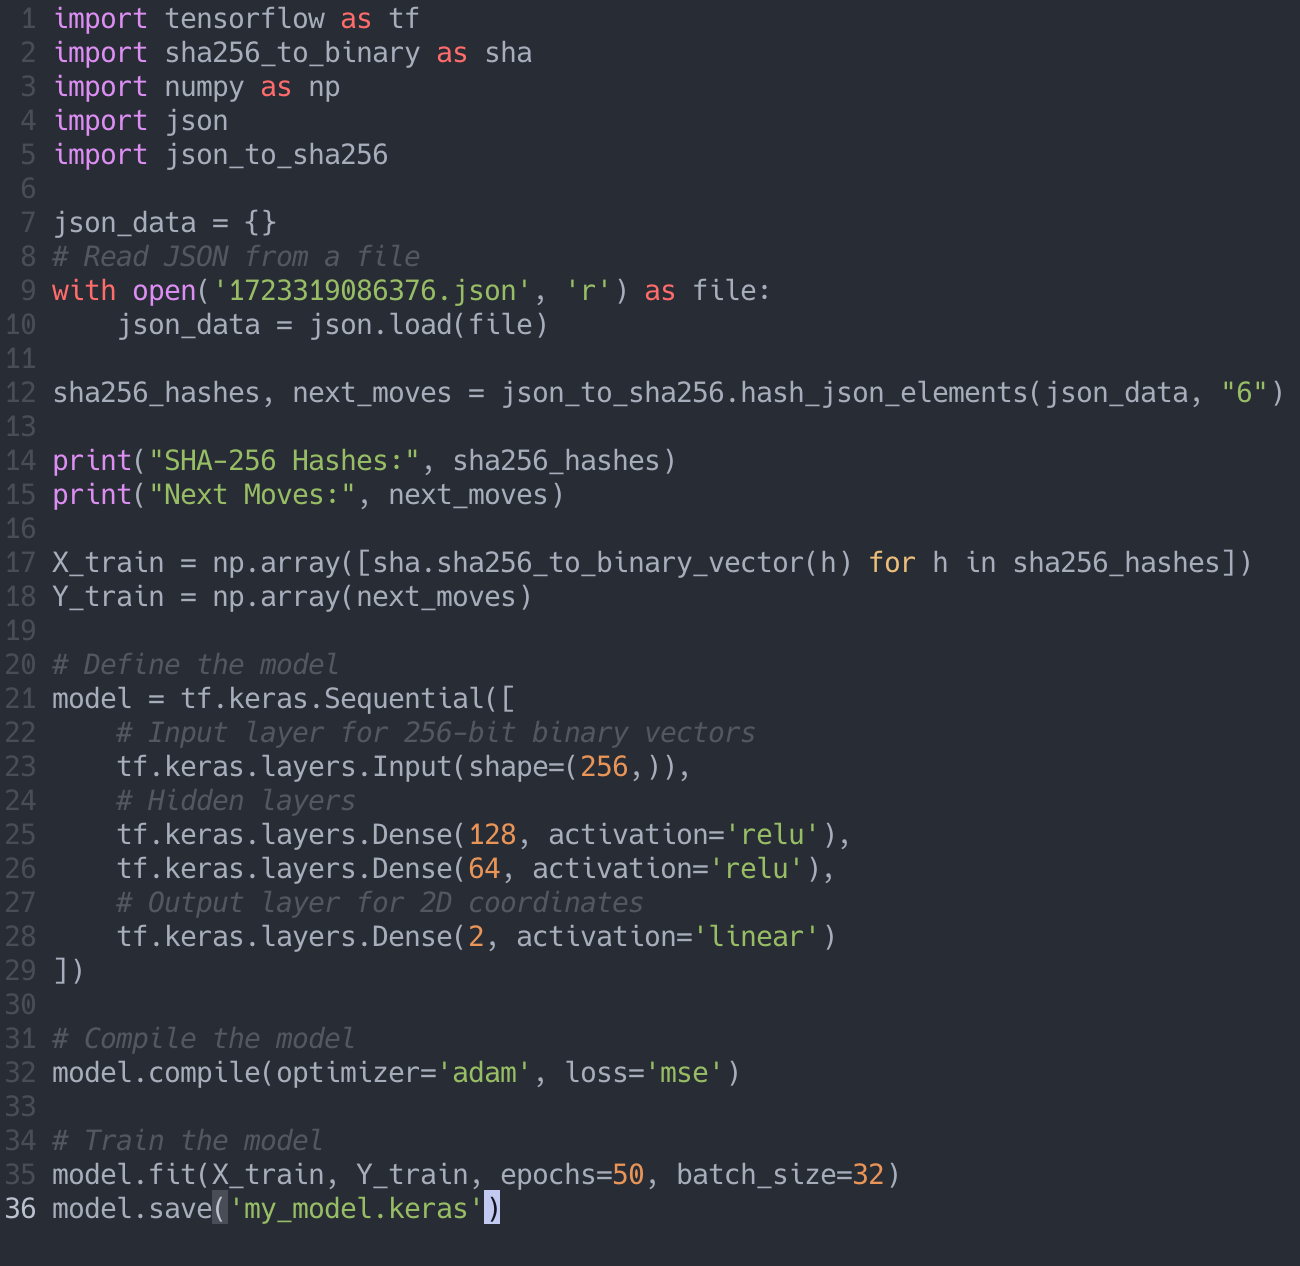
\includegraphics[width=0.75\textwidth]{img/Tensor.png}
    \caption{Kód részlet. A tanító algoritmus}
    \label{code:tensor}
\end{figure}

Az aktivációs függvények célja, hogy nemlinearitást vigyenek a modellbe, lehetővé téve a bonyolult mintázatok felismerését az adatokban. 
Ha nem használnánk aktivációs függvényeket, a modell kimenete csak az inputok egyszerű lineáris kombinációja lenne, ami korlátozná a modell képességeit a komplex kapcsolatok megragadásában.
A ReLU ezért olyan népszerű a mélytanulásban, mert csökkenti gradiensek eltűnésének problémáját, így gyorsabb tanulást és jobb teljesítményt tesz lehetővé.

A kimeneti réteghez egy 2 neuronból álló lineáris aktivációs függvénnyel ellátott réteget használok. A lineáris aktivációs függvény azt jelenti, hogy a neuron kimenete az inputok lineáris kombinációja, ami lényegében nem végez átalakítást. Matematikailag ez így írható le:
\begin{equation}\label{eq:3}
\text{kimenet} = \text{bemenet} \cdot \text{súlyok} + \text{eltolás}
\end{equation}
    

A linear aktivációs függvény használatakor a réteg lényegében nem változtatja meg a bemeneti értékeket, csak a súlyokat és az eltolást alkalmazza.

A modell lefordításához, az $adam$ optimizálót használom, valamint az mse (mean squared error) vagyis az átlagos négyzetes hiba módszert. 
Ez az összeállítás biztosítja, hogy a modell hatékonyan és gyorsan tudjon tanulni a bemeneti adatokból, minimalizálva az előrejelzések és a valós értékek közötti hibát.

\subsection{A modell betanítása}
A modell betanításához szükségem van a hash tömbbé alakított adatokra, valamint ötven tanítási cikluson keresztül az aktuális következő lépések tömbjére. 
Minden edzési lépés során a modell harminckét mintát tartalmazó adatcsomagot dolgoz fel.
Ez a folyamat lehetővé teszi a modell számára, hogy fokozatosan javítson a teljesítményén az adatok ismételt bemutatása és a súlyok frissítése révén. 

A betanított modellt egy \lstinline{my_model.keras} fájlba mentettem le, így könnyen tudtam használni, a játék futtatásakor. 

\section{Modell használata}

\subsection{Python Script API a modell használatához}

Ahhoz, hogy a modellt használni tudjam, egy API-t kellett írnom. Mivel a tesztadatokat is HTTP-kérés segítségével küldtem el, így logikusnak találtam, hogy ezt a megoldást használjam itt is. 

A folyamatot a \ref{code:modell_hasznalata}. ábrával szemléltetem.

\begin{figure}[h]
    \center
    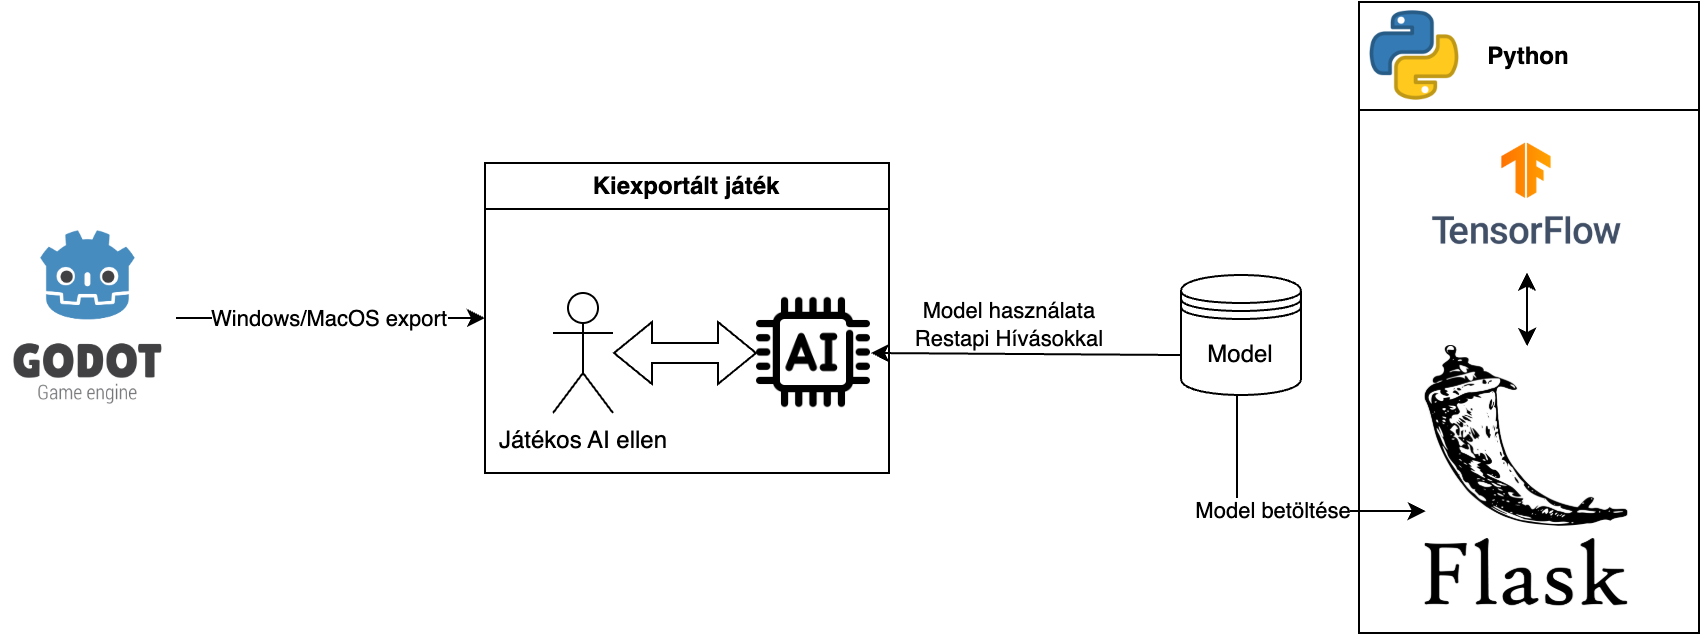
\includegraphics[width=\textwidth]{img/kiexportalt.drawio.png}
    \caption{Diagram. A modell használata.}
    \label{code:modell_hasznalata}
\end{figure}


A Flask használatával készítettem egy webalkalmazást (\ref{code:use_model}. ábra), melynek egyetlen belépési pontja van, a \lstinline{/predict}. A Memória játék ide küldi a \lstinline{POST} HTTP kérését, mely tartalmazza a játék aktuális állását. 
Vagyis az aktuális és az összes eddigi lépést.




\begin{figure}[h]
    \center
    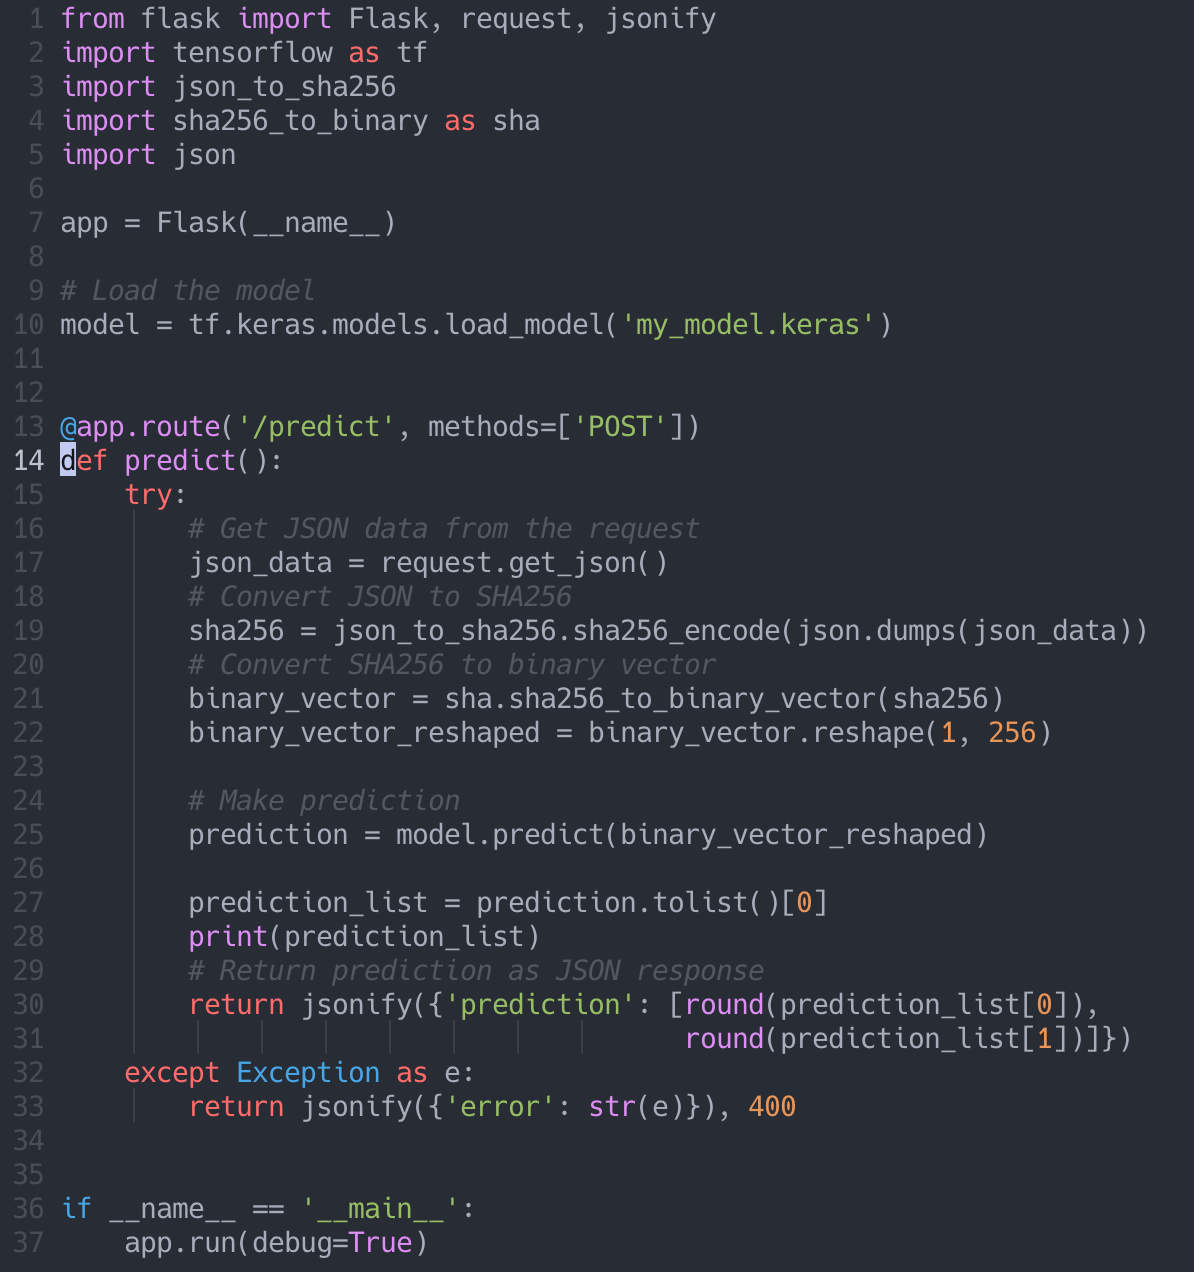
\includegraphics[width=0.75\textwidth]{img/use_model.png}
    \caption{Kód részlet. A modellt használó API}
    \label{code:use_model}
\end{figure}

\subsection{API használata}

Az API indításkor betölti a \lstinline{my_model.keras} fájlból a betanított modellünket, ez percekig is eltart, majd várja a fogadó kéréseket. 
Amikor egy kérés érkezik, a fogadott JSON adatra ráfuttatjuk a már korábban használt SHA256 konvertáló scriptet (\ref{code:json_to_hash}).
Az így kapott 256 hosszú bitsorozattal csinálunk egy "jóslást", vagyis használjuk a modellnek a predict függvényét. Ebből a jóslatból visszakapunk egy két elemű vektort, melynek elemei nem egész számok.

Mivel két pozitív egész számra, azaz koordinátára van szükségünk, a kapott értékeket kerekítjük, majd HTTP-válaszként visszaküldjük a két egész számot.
\subsection{Játék kódjában való változtatások}

A játékot, ahhoz hogy működjön a mesterséges inteligenciával, először át kellett alakítanom, hogy minden lépésem után az MI következzen. A változtatás egyszerű volt: egy változóba tárolom, hogy a játékos, vagy az MI köre van soron, és minden pár fordítása után cserélem. 

Ahhoz, hogy az MI is tudjon kártyát választani, készítettem egy \lstinline{get_ai_cards} függvényt (\ref{code:get_ai_card}. ábra). A függvény meghívja a \lstinline{\prediction} végpontot, a \lstinline{HttpClient} segítségével.
A visszakapott koordinátákból kiválasztja a kártyát az asztalon. 
Ha ez a kártya nem elérhető, mert már levették az asztalról, vagy a koordináták nem létező kártyára mutatnak, akkor a legelső elérhető kártyát fogja választani a mesterséges intelligencia. 

\begin{figure}[H]
    \centering
    \begin{lstlisting}[language=GDScript]
func get_ai_cards():
        var output;
        waiting_for_card=true;
        if data.card_selections:
            output = HttpClient.post_JSON_tensor(data.card_selections);
            waiting_for_card=false
            if output:
                var coord_x:int=output["prediction"][0]
                var coord_y:int=output["prediction"][1]
                var Card=cards[0];
                for c in cards:
                    if c.table_x==coord_x && c.table_y==coord_y:
                        Card=c
                return Card
    \end{lstlisting}
    \caption{Kód részlet: Az MI kártya választó függvénye GDScript-ben.}
    \label{code:get_ai_card}
\end{figure}


	\chapter{Tesztelési eredmények}

\thispagestyle{fancy}
\pagestyle{fancy}

A témavezetőm segítségével a kész projektemet, mely már tartalmazta a mesterséges inteligenciát is,  sikerült az egyetem hallgatóival teszteltetni.
A teszt eredményeit a User Experience Questionnaire (Felhasználói Élmény Kérdőív, röviden UEQ) adat-elemző eszközzel, valamint a System Usability Scale (Rendszer Használhatósági Skála, azaz SUS) segítségével értékeltük ki. 

\section{Demográfiai adatok}
A szakdolgozatom tesztelő egyetemi hallgatók demográfiai adatok a \ref{tab:demografia} táblázatban láthatók. A tesztelés célja az alkalmazás funkcionalitásának és használhatóságának értékelése volt. A résztvevők visszajelzéseit gyűjtöttük, és ezen észrevételek alapján a jövőben tervezzük a program finomítását.

\vspace{1cm}

\begin{table}[!h]
    \caption{Demográfiai adatok}
    \label{tab:demografia}
    \resizebox{\linewidth}{!}{%
    \begin{tabular}{ccccccc} % specify the number of columns
    \hline
    \multicolumn{1}{c}{\textbf{ID}} & 
    \multicolumn{1}{c}{\textbf{Korcsoport}} & 
    \multicolumn{1}{c}{\textbf{Nem}} & 
    \multicolumn{1}{c}{\textbf{Legmagasabb iskola}} & 
    \multicolumn{1}{c}{\textbf{Techn. Járt.}} & 
    \multicolumn{1}{c}{\textbf{Elsődleges játékhoz}} & 
    \multicolumn{1}{c}{\textbf{Oktatásban töltött évek száma}} \\ \hline
    
    1 & 18-24 & Férfi & Középiskola & Haladó & Asztali számítógép & 13 \\
    2 & 25-34 & Férfi & Középiskola & Középhaladó & Laptop & 18 \\
    3 & 18-24 & Férfi & Technikus & Kezdő & Laptop & 14 \\
    4 & 18-24 & Férfi & Technikus & Haladó & Asztali számítógép & 13 \\
    5 & 18-24 & Férfi & Középiskola & Középhaladó & Asztali számítógép & 16 \\
    6 & 18-24 & Férfi & Középiskola & Kezdő & Asztali számítógép & 14 \\
    7 & 18-24 & Férfi & Középiskola & Középhaladó & Asztali számítógép & 15 \\
    8 & 18-24 & Férfi & Középiskola & Haladó & Asztali számítógép & 16 \\
    9 & 18-24 & Férfi & Középiskola & Haladó & Asztali számítógép & 13 \\
    10 & 25-34 & Férfi & Mesterfokozat & Szakértő & Okostelefon & 20 \\
    11 & 25-34 & Férfi & Főiskolai diploma & Szakértő & Asztali számítógép & 17 \\
    
    \hline
    \end{tabular}%
    }
    \end{table}

\section{UEQ - User Experience Questionnaire}


A \textit{User Experience Questionnaire} (UEQ) egy gyakran használt eszköz, amely lehetővé teszi a termékek és szolgáltatások felhasználói élményének mérését. Az UEQ kifejezetten úgy lett kialakítva, hogy gyorsan és hatékonyan nyújtson visszajelzést a felhasználói élmény különböző aspektusairól, mint például a használhatóság, az esztétika és az érzelmi hatások.

\subsection{Kérdőív felépítése és dimenziói}

Az UEQ kérdőív 26 tételből áll, amelyeket hat különböző dimenzióra osztanak:

\begin{itemize}
    \item \textbf{Vonzalom (Attractiveness)}: Az általános benyomás és az érzelmi reakció a termékre vagy szolgáltatásra.
    \item \textbf{Megértés (Perspicuity)}: A termék vagy szolgáltatás használatának egyszerűsége és könnyű megértése.
    \item \textbf{Hatékonyság (Efficiency)}: A feladatok gyors és hatékony végrehajtásának képessége.
    \item \textbf{Szervezettség (Dependability)}: Az irányítás érzete és a rendszer kiszámíthatósága.
    \item \textbf{Stimuláció (Stimulation)}: A termék vagy szolgáltatás által nyújtott inspiráció és motiváció.
    \item \textbf{Újdonság (Novelty)}: Az innováció érzete és a termék vagy szolgáltatás újszerűsége.
\end{itemize}

A következő megállapításokat tehetjük a különböző értékelésekről és azok szerepéről a mi esetünkben:

\begin{itemize}
    \item \textbf{Semleges értékelés (-0,8 és 0,8 között):} Ez a tartomány a skála viszonylag semleges megítélését jelzi. Ilyen értékek esetén az eredmények nem mutatnak kiemelkedő pozitív vagy negatív irányt.
    
    \item \textbf{Pozitív értékelés (> 0,8):} Ezek az értékek pozitív megítélést jelentenek. A mi esetünkben, ha a skálán +0,8 feletti értékek szerepelnek, az azt jelzi, hogy a vizsgált jellemzők kedvezőek és pozitív benyomást keltenek.
    
    \item \textbf{Negatív értékelés (< -0,8):} Ezek az értékek negatív értékelést tükröznek. Ha a skála -0,8 alatti értékeket mutat, az a vizsgált jellemzők kedvezőtlen megítélésére utal.
    
    \item \textbf{Skálatartomány:} A skála értékeinek teljes tartománya -3 (nagyon rossz) és +3 (nagyon jó) között mozog. A valós alkalmazásokban a legtöbb esetben a -2 és +2 közötti értékekkel találkozunk, mivel az extrém válaszok ritkán fordulnak elő.
\end{itemize}

\subsection{Kiértékelés}
\begin{table}[h]
    \centering
    \caption{UEQ skála, Átlag és szórás}
    \begin{tabular}{|l|c|c|}
        \hline
        \textbf{Skála} & \textbf{Átlag} & \textbf{Szórás} \\ \hline
        Kellem & 1.167 & 0.53 \\ \hline
        Áttekinthetőség & 2.364 & 0.74 \\ \hline
        Hatékonyság & 0.750 & 0.59 \\ \hline
        Megbízhatóság & 1.136 & 1.08 \\ \hline
        Ösztönzés & 1.159 & 0.63 \\ \hline
        Újszerűség & 0.500 & 0.78 \\ \hline
    \end{tabular}
    \label{tab:ueq_scales}
\end{table}

\begin{figure}[h]
    \center
    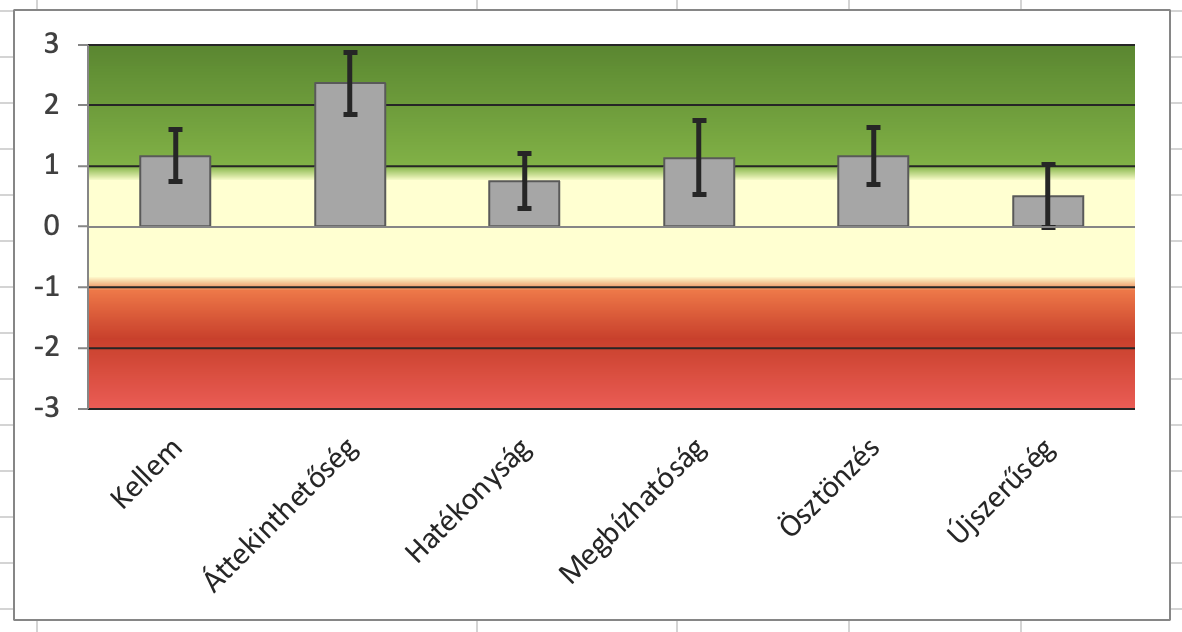
\includegraphics[width=0.75\textwidth]{img/UEQ_diagram.png}
    \caption{UEQ diagram eredmények}
    \label{diag:ueq}
\end{figure}

A \ref{tab:ueq_scales} táblázat adatai alapján, a hatból 4 dimenzióban jól teljesített  programom, Áttekinthetősségben kiemelkedően, és csak a Hatékonyság és az Újszerűség az, ahol neutrálisak az értékek. A \ref{diag:ueq}. ábra jól szemlélteti ezt. 


A UEQ skáláit a következő két fő kategóriába sorolhatjuk: pragmatikus minőség (amely magában foglalja az Áttekinthetőséget, Hatékonyságot és Megbízhatóságot) és hedonikus minőség (Ösztönzés és Újszerűség). 
Míg a pragmatikus minőség a feladatokhoz kapcsolódó minőségi szempontokat értékeli, addig a hedonikus minőség a nem feladatorientált minőségi tényezőkre fókuszál.

A \ref{tab:pragmatic_hedonic_quality}. táblázatban a \textit{kellemes} a három \textit{pragmatikus} és a két \textit{hedonikus} minőség szempont átlagértéke kerül kiszámításra. 

\begin{table}[h]
    \centering
    \caption{Pragmatikus és hedonikus minőségek}
    \begin{tabular}{|l|c|}
        \hline
        \textbf{Kategória} & \textbf{Érték} \\ \hline
        Kellem & 1.17 \\ \hline
        Pragmatikus minőség & 1.42 \\ \hline
        Hedonikus minőség & 0.83 \\ \hline
    \end{tabular}
    \label{tab:pragmatic_hedonic_quality}
\end{table}

Megvizsgálva az értékeket, boldogan tapasztaltam, hogy mind a három csoportban pozitív eredményt érhettem el, noha a Hedonikus értékekben épp csak megütöttem a 0.83-al. Ezt a \ref{diag:pragmatic_hedonic}. ábrában is láthattuk.

Kimagaslóan jó eredményem lett a pragmatikus minőségekből, amiből én arra következtettem, hogy a programom a feladatát megfelelően végzi el. 

A memóriajáték fejlesztése során a jövőben kiemelt figyelmet kell fordítani az újszerűségre, mivel ez hozzájárulhat a hedonikus minőség javításához is. Ezt valamilyen innovatív megoldással tudnám a legkönnyebben elérni.

\begin{figure}[h]
    \center
    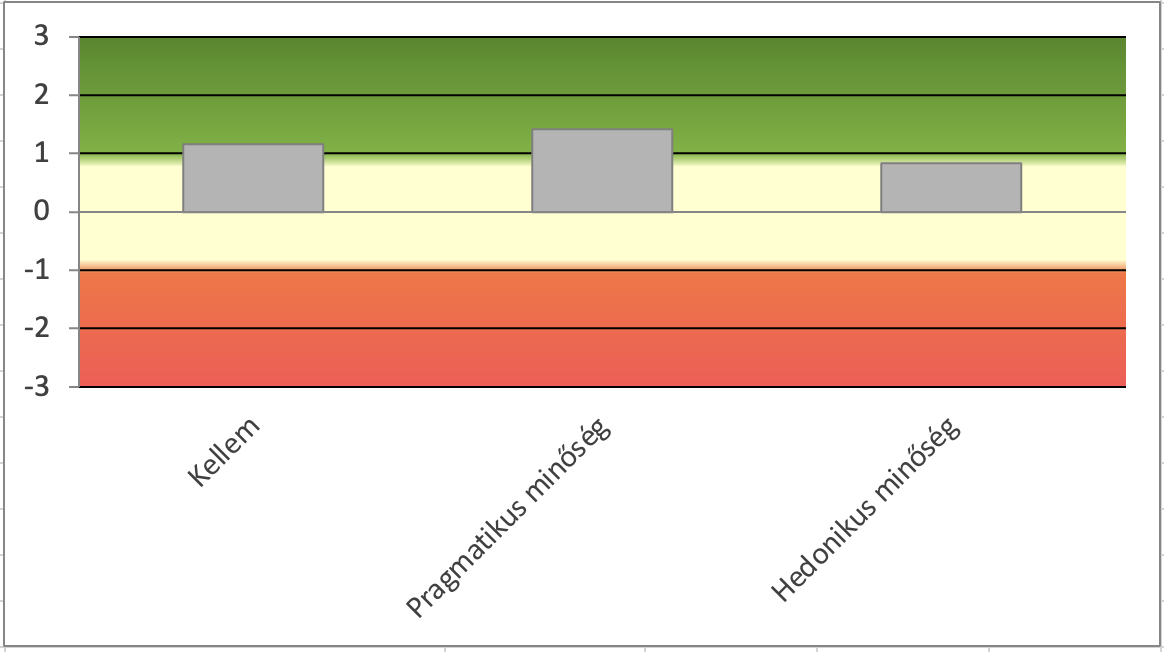
\includegraphics[width=0.75\textwidth]{img/UEQ_pragmatic_hedonic.png}
    \caption{Diagram: UEQ pragmatikus és hedonikus minőségek}
    \label{diag:pragmatic_hedonic}
\end{figure}

\section{SUS - System Usability Scale}

A SUS (System Usability Scale), magyarul Rendszerhasználhatósági Skála, egy rövid, tíz kérdésből álló kérdőív, amely a rendszerek, termékek vagy szolgáltatások használhatóságának gyors és hatékony értékelésére szolgál. 
A kérdőív célja, hogy visszajelzést adjon a felhasználói élményről és az általános elégedettségről.

\subsection{Működési Elv}
\begin{enumerate}
    \item \textbf{Kérdések:} A SUS kérdőív 10 állítást tartalmaz, amelyek a rendszer használhatóságával kapcsolatosak. A kérdések között találhatóak pozitív (pl. ``Azt hiszem, szeretném gyakran használni ezt a rendszert.'') és negatív (pl. ``Azt tapasztaltam, hogy a rendszer szükségtelenül bonyolult.'') megfogalmazású kijelentések.
    
    \item \textbf{Értékelés:} A válaszadók 5 pontos skálán (1-től 5-ig) értékelik az állításokat. A skála 1 = ``Teljesen nem értek egyet'' és 5 = ``Teljesen egyetértek'' közötti értékeket használja.
    
    \item \textbf{Számítás:} A válaszok értékelése során a pozitív állításoknál 1-gyel csökkentik a adott értékelést, majd ezt az értéket kivonják 5-ből. A negatív állításoknál az értékelést egyszerűen levonják 1-ből. A végső pontszám kiszámításához az összes állítás eredményeit összeadják, majd ezt az értéket megszorozzák 2.5-tel, így egy 0-tól 100-ig terjedő skálán kaphatunk eredményt.
    
    \item \textbf{Értelmezés:} Az eredményként kapott pontszám a termék vagy rendszer általános használhatóságának értékelését szolgálja. A 68 körüli átlagpontszám jó használhatóságot jelez, míg az ennél alacsonyabb értékek esetében problémákra lehet következtetni.
\end{enumerate}

\subsection{Kérdések és a válaszok}
A tíz kérdésem/kijelentésem, a következők voltak:

\begin{enumerate}
    \item Azt hiszem, szeretném gyakran használni ezt a rendszert.
    \item Azt tapasztaltam, hogy a rendszer szükségtelenül bonyolult.
    \item Úgy gondoltam, hogy a rendszer könnyen használható.
    \item Azt hiszem, szükségem lenne egy műszaki szakember támogatására ahhoz, hogy használni tudjam ezt a rendszert.
    \item Úgy találtam, hogy a rendszer különböző funkciói jól integráltak.
    \item Úgy éreztem, hogy túl sok ellentmondás van ebben a rendszerben.
    \item Azt képzelem, hogy a legtöbb ember nagyon gyorsan megtanulná használni ezt a rendszert.
    \item Azt tapasztaltam, hogy a rendszer nagyon nehézkes a használat során.
    \item Nagyon magabiztosan éreztem magam a rendszer használata közben.
    \item Sokat kellett tanulnom, mielőtt elkezdhettem volna használni ezt a rendszert.
\end{enumerate}

\begin{table}[h]
    \centering
    \begin{tabular}{|c|c|c|c|c|c|c|c|c|c|c|}
        \hline
        ID & 1 & 2 & 3 & 4 & 5 & 6 & 7 & 8 & 9 & 10 \\ \hline
        1  & 2 & 4 & 2 & 2 & 3 & 2 & 4 & 2 & 4 & 2  \\ \hline
        2  & 4 & 1 & 5 & 1 & 4 & 1 & 5 & 1 & 5 & 1  \\ \hline
        3  & 3 & 1 & 5 & 1 & 3 & 1 & 5 & 1 & 5 & 1  \\ \hline
        4  & 3 & 1 & 5 & 1 & 4 & 1 & 5 & 1 & 4 & 1  \\ \hline
        5  & 5 & 1 & 1 & 2 & 2 & 3 & 2 & 2 & 3 & 2  \\ \hline
        6  & 2 & 2 & 4 & 2 & 3 & 2 & 5 & 1 & 4 & 1  \\ \hline
        7  & 5 & 1 & 5 & 1 & 5 & 1 & 5 & 1 & 5 & 1  \\ \hline
        8  & 4 & 1 & 5 & 3 & 3 & 1 & 5 & 1 & 5 & 1  \\ \hline
        9  & 1 & 1 & 5 & 1 & 5 & 1 & 5 & 1 & 5 & 1  \\ \hline
        10 & 1 & 1 & 5 & 2 & 5 & 1 & 5 & 1 & 5 & 1  \\ \hline
        11 & 2 & 1 & 5 & 3 & 3 & 2 & 4 & 1 & 5 & 1  \\ \hline
    \end{tabular}
    \caption{Válaszok}
    \label{tab:sus_data}
\end{table}

A kiértékeléshez a System Usability Scale Analysis Toolkit-et \cite{SUSAnaly62:online} használtam, mellyel a következő eredmények jöttek ki a \ref{tab:sus_data}. táblázat értékeire. 

\begin{itemize}
    \item \textbf{SUS Tanulmány Pontszám:} 82.5
    \item \textbf{Medián:} 87.5
    \item \textbf{Szórás:} 14.19
    \item \textbf{Jellemző:} Kiváló
    \item \textbf{Osztályzat:} A
    \item \textbf{Elfogadhatóság:} Elfogadható
    \item \textbf{Negyed:} 4. negyed
\end{itemize}

\begin{figure}[h]
    \center
    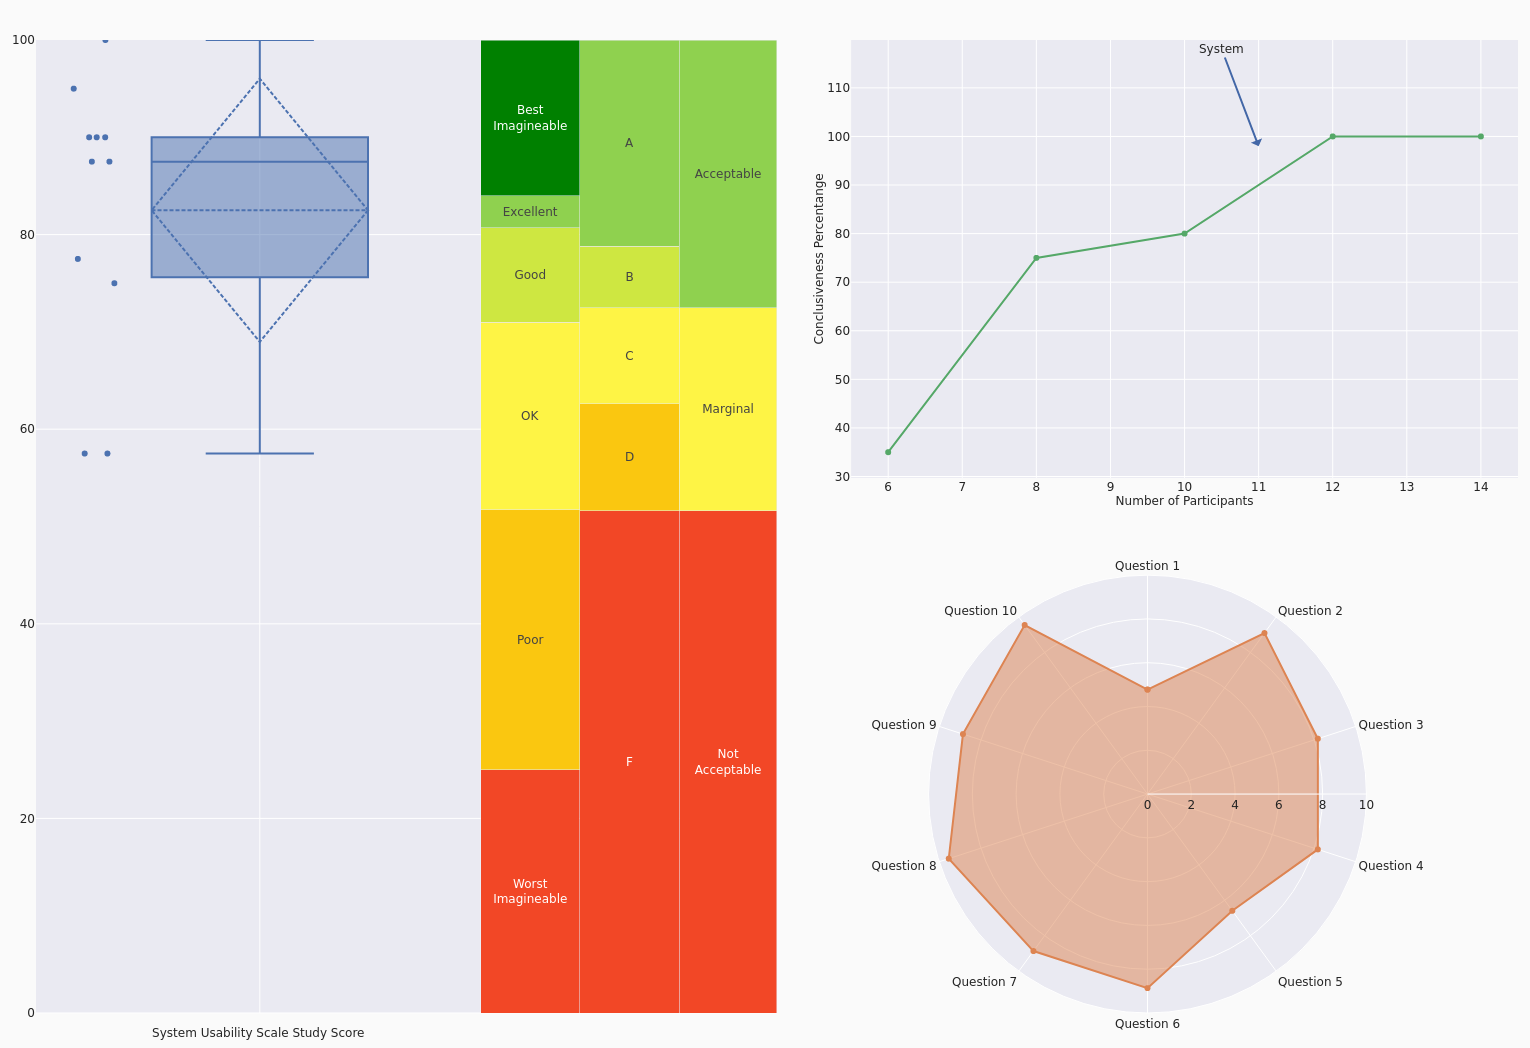
\includegraphics[width=\textwidth]{img/single_study_plot.png}
    \caption{SUS táblázat kiértékelt eredményei}
    \label{diag:sus_result}
\end{figure}

A diagrammon (\ref{diag:sus_result}. ábra) jól látszik, hogy az első és az ötödik kérdésekben a memória játékom alul teljesített. Az első kérdés, amely arra vonatkozik, hogy a felhasználók mennyire szeretnék gyakran használni a játékot, azt mutatja, hogy a válaszadók viszonylag alacsony érdeklődést mutatnak a rendszer rendszeres használata iránt.
 Ez aggasztó, mivel a gyakori használat egy fontos indikátora lehet a játék élvezhetőségének és vonzerejének.

Az ötödik kérdés kapcsán a felhasználók átlagos minőségűnek ítélték a megvalósítást, ami arra utal, hogy a játék nem hagyott maradandó benyomást, és nem tudta felkelteni a felhasználók érdeklődését olyan mértékben, hogy kiemelkedő minőséget mutasson.
 Ez a fajta közepes értékelés azt jelzi, hogy bár a játék elér egy bizonyos szintet, van még lehetőség a fejlődésre.

Mindkét területen – a felhasználói élmény fokozásában és a játék minőségének javításában – jelentős potenciál rejlik.
Fontos lenne részletesen elemezni, hogy mik azok a konkrét elemek, amelyek nem nyerték el a felhasználók tetszését.
Lehetséges, hogy a játékmenet, a grafika vagy akár a hangzásvilág is hozzájárulhat ehhez az érzéshez.
A felhasználói visszajelzések figyelembevételével, valamint alapos tesztelésekkel képesek lehetünk a szükséges módosításokat végrehajtani, így a játék vonzereje és használhatósága jelentősen javulhat.

Ezeket a problémákat kezelve, a jövőbeni fejlesztések során érdemes lenne a felhasználói élményt a középpontba állítani, hiszen egy élvezetes és vonzó játék ösztönzi a felhasználókat a rendszeres visszatérésre és a játék gyakori használatára


	\chapter{Összefoglaló}

\thispagestyle{fancy}
\pagestyle{fancy}

Összességében sikerült létrehoznom egy memóriajátékot a Godot Engine segítségével, és sikeresen begyűjtöttem elegendő tesztadatot ahhoz, hogy a játék működjön a mesterséges intelligencia ellen. A projekt során értékes tapasztalatokat szereztem, amelyek segítettek a program fejlesztésében.

A játék azonban még fejlődési lehetőségeket rejt magában. Elsősorban a mesterséges intelligencia modelljét érdemes lenne tovább finomítani. Esetleg egy összetettebb tanítási mintával is megpróbálhatnám betanítani, hogy a rendszer jobban alkalmazkodjon a játék dinamikájához. Emellett a kimeneti mintát is érdemes lenne javítani: ahelyett, hogy csak egy kártyát fordítana fel, a rendszer egy valószínűségi táblát is adhatna vissza, amely megmutatja, hogy a különböző kártyák milyen valószínűséggel kerülnek felfordításra a játék során. Ez a megközelítés növelheti az MI stratégiájának komplexitását és versenyképességét.

Továbbá az élvezeti faktort is érdemes lenne növelni. Például bevezethetünk egy pontrendszert, amely világosan jelzi, hogy a játékos és a mesterséges intelligencia hány ponttal zárta a játékot. Ez nemcsak az izgalmat fokozná, hanem motiválhatná a játékosokat a teljesítményük javítására is.

A projektből az a tanulság vonható le, hogy gyakran a legegyszerűbbnek tűnő feladatok jelentették a legnagyobb kihívást a projekt során. Az apró részletek és finomítások, amelyek elsőre jelentéktelennek tűntek, kulcsszerepet játszottak a játék élvezhetőségében és funkcionalitásában. Ezt a tapasztalatot a jövőbeli projekteknél is hasznosítani fogom.


	
	%Irodalomjegyzék generálása a dolgozatba a következő sorok hatására történik, szerkeszteni nem kell. A hivatkozott források gyűjteményét a mybib.bib nevű fájlban kell kialakítani a mintáknak megfelelő formátumban
	\bibliography{mybib}
	\pagestyle{plain}
	\addcontentsline{toc}{chapter}{Irodalomjegyzék}
	%megjelenés sorrendjében építi fel az irodalomjegyzéket
	\bibliographystyle{ieeetr}
	% a következő sor a dolgozat digitális mellékletének a tartalmát csatolja a dolgozathoz, ezt a fájllistát a files.tex fájlban kell megírni
	\chapter{Mellékletek}
\thispagestyle{fancy}
\pagestyle{fancy}

\thispagestyle{fancy}
\pagestyle{fancy}

\subsubsection{Beadott fájlok}
\noindent 3D-memoria-jatek-mestereseges-inteligenciaval mappa (a szoftver fájljai):\\
\begin{tabular}{l l}
    \quad icon.svg  & \quad Godot alapértelmezett ikonja a játékhoz \\ 
    \quad icon.svg.import  & \quad Godot metaadat \\ 
    \quad openxr\_action\_map.tres & \quad OpenXR metaadat \\ 
    \quad project.godot  & \quad Godot projekt fájl \\ 
\end{tabular}
\\\\
\noindent 3D-memoria-jatek-mestereseges-inteligenciaval/Animations mappa (a szoftver animációs fájlok):\\
\begin{tabular}{l l}
    \quad Idle.res  & \quad Kártya animáció \\ 
    \quad Megfordit.res  & \quad Kártya megfordít animáció \\ 
    \quad RESET.res  & \quad Kártya Reset animáció \\
\end{tabular}
\\\\
\noindent 3D-memoria-jatek-mestereseges-inteligenciaval/Scenes mappa (a szoftver jelenetei):\\
\begin{tabular}{l l} 
    \quad MainScrenes  & \quad Fő jelenet\\ 
    \quad MenuScene.tscn  & \quad Főmenü jelenet \\ 
    \quad XrOrigin.tscn  & \quad XR kezdőjelenet \\ 
    \quad button.tscn  & \quad Gomb jelenet \\ 
    \quad plainField.tscn  & \quad Üres tér jelenet \\ 
    \quad plain\_camera.tscn  & \quad Kamera jelenet \\ 
    \quad basics.tscn  & \quad Alapok jelenet \\ 
    \quad Card.gdshader  & \quad Kártya shader\\ 
    \quad Card.tscn  & \quad Kártya jelenet\\ 
    \quad Outline.gdshader  & \quad Kártya körvonal shader\\ 
\end{tabular}

\newpage

\noindent 3D-memoria-jatek-mestereseges-inteligenciaval/Scripts mappa (a szoftver GDScript szkriptjei):\\
\begin{tabular}{l l}
    \quad Card.gd  & \quad Kártya jelenet szkriptje \\ 
    \quad Deck.gd  & \quad Paklik jelenet szkriptje \\ 
    \quad InputField.gd  & \quad Bemeneti mező szkript \\ 
    \quad MenuScene.gd  & \quad Menü jelenet szkriptje \\ 
    \quad VrScript.gd  & \quad VR specifikus szkript \\ 
    \quad basics.gd  & \quad Alap jelent szrikptje \\ 
    \quad button.gd  & \quad Gomb jelent szriptje \\ 
    \quad constant.gd  & \quad Állandók definiálásra használt szkript \\ 
    \quad deck\_timer.gd  & \quad Pakli időzítő szkript \\ 
    \quad http\_client.gd  & \quad HTTP kérések kezelése szkript \\ 
    \quad player\_data.gd  & \quad Játékos adatainak tárolására használt adatszerkezet definiáló szript \\ 
    \quad scene\_manager.gd  & \quad Jelenet váltást kezelő szkript \\ 
\end{tabular}
\\\\
\noindent 3D-memoria-jatek-mestereseges-inteligenciaval/Shaders mappa (A játék grafikai megjelenítését szolgáló fájlok): \\
\begin{tabular}{l l}
    \quad MenuScene.tres  & \quad Menű kinézetét szolgáló shader könyvtár\\ 
    \quad cardTestLibary.tres  & \quad Egy teszt saját shader könyvtár tesztje \\ 
    \quad new\_standard\_material\_3d.tres  & \quad A Gombokhoz használt shader könyvtár \\     
\end{tabular}
\\\\
\noindent 3D-memoria-jatek-mestereseges-inteligenciaval/Templates mappa: \\
\begin{tabular}{l l}
    \quad custom\_build\_template.html  & \quad A HTML exporthoz használt saját html template\\ 
\end{tabular}
\\
\\
\noindent 3D-memoria-jatek-mestereseges-inteligenciaval/fileServer mappa: (Adatok gyüjtését szolgáló fájlszerver) \\
\begin{tabular}{l l}
    \quad Dockerfile  & \quad Docker konténer buildelését szolgáló fájl \\ 
    \quad docker-compose.yaml  & \quad Docker kontérek kezelését szolgáló compose fájl \\ 
    \quad package-lock.json  & \quad Node.JS package-lock fájl, npm használja\\ 
    \quad package.json  & \quad Node.JS package fájl, npm használja. \\ 
    \quad server.js  & \quad Fájlszerver forráskódja \\ 
\end{tabular}

\newpage

\noindent 3D-memoria-jatek-mestereseges-inteligenciaval/tensorflow: (Az MI modell használatához és tanításához szükséges fájlok.) \\
\begin{tabular}{l l}
    \quad json\_to\_sha256.py  & \quad JSON adatok SHA256 konvertálását szolgáló Python szkript \\ 
    \quad my\_model.keras  & \quad A betanított és  mentett MI modell \\ 
    \quad sha256\_to\_binary.py  & \quad SHA256 hash konvertálása bitekre Python szkript \\ 
    \quad tensor.py  & \quad TensorFlow tanító algoritmus, MI betanítása szkript \\ 
    \quad use\_model.py  & \quad Flask szerver, az MI modell használata Python szkript\\ 
\end{tabular}
\\
\\
\noindent SAS\_UEQ mappa (Teszteredmények XLSX fájlai): \\
\begin{tabular}{l l}
    \quad UEQ\_Data\_Analysis\_Tool\_Version12.xlsx & \quad UEQ teszt eredmények XLSX \\
    \quad SAS\_teszt.xlsx & \quad SAS teszt eredmények XLSX \\
\end{tabular}
\\
\\
\noindent p8mqg2\_tex mappa (tex fájlok és képek): \\
\begin{tabular}{l l}
    \quad 4x4\_all\_card\_fliped.png & \quad\quad\quad menu.png\\
    \quad Itch.io.png & \quad\quad\quad menu\_remake.png\\
    \quad JSON.png & \quad\quad\quad menu\_scene\_tree.png\\
    \quad JSON\_TO\_SHA256.png & \quad\quad\quad single\_study\_plot.png\\
    \quad Tensor.png & \quad\quad\quad use\_model.png\\
    \quad UEQ\_diagram.png & \quad\quad\quad Fejezet1.tex\\
    \quad UEQ\_pragmatic\_hedonic.png & \quad\quad\quad Fejezet2.tex\\
    \quad adatgyujtes.png & \quad\quad\quad Fejezet3.tex\\
    \quad allapotgep.png & \quad\quad\quad Fejezet4.tex\\
    \quad animation\_tree.png & \quad\quad\quad Fejezet5.tex\\
    \quad asztal\_4x4.png & \quad\quad\quad Fejezet6.tex\\
    \quad asztal\_4x4\_card\_flipped.png & \quad\quad\quad Fejezet7.tex\\
    \quad asztal\_4x4\_non\_pair.png & \quad\quad\quad Fejezet8.tex\\
    \quad asztal\_4x4\_pair.png & \quad\quad\quad folyamat\_diagram.tex\\
    \quad asztal\_4x4\_pair\_eltunik.png & \quad\quad\quad Abstract.tex\\
    \quad basic\_field\_scene\_structure.png & \quad\quad\quad Fedlap.tex\\
    \quad cards\_scene\_tree.png & \quad\quad\quad Jelolesjegyzek.tex\\
    \quad cloudflair-censored.jpg & \quad\quad\quad Koszonetnyilvanitas.tex\\
    \quad fullfolyamat.jpg & \quad\quad\quad files.tex\\
    \quad fullfolyamat.png & \quad\quad\quad h\_nyilatkozat.tex\\
    \quad hash\_to\_bit.png & \quad\quad\quad tv\_nyilatkozat.tex\\
    \quad kiexportalt.drawio.png & \quad\quad\quad\\
\end{tabular}
\vspace{28pt}


	% a dolgozatban az ábrajegyzéket el kell helyezni, ezt a TeX automatikusan előállítja és a következő sor határása elhelyezi a dokumentumban
	\listoffigures
	%Ha vannak táblázatok is, akkor ezeket is listába gyűjtjük, és a következő utasítással az ábrajegyzéket követően a dolgozatba legeneráltatjuk. Ha nincs rá szükség, a százalék jellel a sor elején érvénytelenítjük a parancsot vagy töröljük a sort
	\listoftables
	
	
\end{document}
